\documentclass[12pt, letterpaper]{report}
\setlength{\parindent}{0pt}
\usepackage[italian]{babel}
\usepackage[most]{tcolorbox}
\usepackage{amsthm}
\usepackage{amsmath}
\usepackage{tabularx}
\usepackage{amssymb}
\usepackage{enumitem}
\usepackage{amsfonts}
\usepackage{centernot}
\usepackage{wrapfig}
\usepackage{circuitikz}
\usepackage{float}
\usepackage{multirow}
\usepackage{karnaugh-map}
\usepackage{listings}
\usepackage{verbatim}
\usepackage{hyperref}
\setlist[enumerate]{label*=\arabic*.}
\usepackage{bbm}
\title{Sistemi operativi}
\date{}
\setcounter{chapter}{0}
\definecolor{brickred}{RGB}{182, 50, 28}
\definecolor{darkred}{RGB}{139, 0, 0}
\definecolor{brickred}{RGB}{182, 50, 28}
\definecolor{darkred}{RGB}{139, 0, 0}
\definecolor{codegreen}{rgb}{0,0.6,0}
\definecolor{codegray}{rgb}{0.5,0.5,0.5}
\definecolor{codepurple}{rgb}{0.58,0,0.82}
\definecolor{backcolour}{rgb}{0.95,0.95,0.92}
\definecolor{darkblue}{rgb}{0,0,0.6}
\hypersetup{
	colorlinks=true,
	linkcolor=darkred,
	filecolor=darkred,
	urlcolor=darkred
}

\lstdefinestyle{pascalstyle}{
	backgroundcolor=\color{backcolour},   
	commentstyle=\color{codegreen},
	keywordstyle=\color{blue}\bfseries,
	numberstyle=\tiny\color{codegray},
	stringstyle=\color{codepurple},
	basicstyle=\ttfamily\footnotesize,
	breakatwhitespace=false,         
	breaklines=true,                 
	captionpos=b,                    
	keepspaces=true,                 
	numbers=left,                    
	numbersep=5pt,                  
	showspaces=false,                
	showstringspaces=false,
	showtabs=false,                  
	tabsize=2,
	language=C++
}

\newcounter{theorem}
\newcounter{lemma}
\newcounter{corollary}
\newcounter{definition}
\newcounter{exercise}


\labelformat{theorem}{teorema #1}
\labelformat{lemma}{lemma #1}
\labelformat{corollary}{corollario #1}
\labelformat{definition}{definizione #1}
\labelformat{note}{nota #1}
\labelformat{example}{esempio #1}
\labelformat{exercise}{esercizio #1}

\newtcbtheorem[number within=chapter,use counter=theorem]{theorem}%
{Teorema}{arc=1mm,outer arc=1mm,colframe=cyan!55!black,fonttitle=\scshape,lefttitle=1mm,separator sign dash,description font=\bfseries,description delimiters={\flqq}{\frqq}}{th}

\newtcbtheorem[number within=theorem,use counter=corollary]{corollary}%
{Corollario}{arc=1mm,outer arc=1mm,colframe=cyan!55!black,fonttitle=\scshape,lefttitle=1mm,separator sign dash,description font=\bfseries,description delimiters={\flqq}{\frqq}}{cor}

\newtcbtheorem[number within=chapter,use counter=lemma]{lemma}%
{Lemma}{arc=1mm,outer arc=1mm,colframe=cyan!55!black,fonttitle=\scshape,lefttitle=1mm,separator sign dash,description font=\bfseries,description delimiters={\flqq}{\frqq}}{lem}

\newtcbtheorem[number within=chapter,use counter=definition]{definition}%
{Definizione}{breakable, enhanced, arc=1mm,outer arc=1mm,colframe=green!55!black,fonttitle=\scshape,separator sign dash,description font=\bfseries,description delimiters={\flqq}{\frqq}}{def}

\newtcbtheorem[no counter]
{note}{Nota}{blanker,breakable,left=5mm,before skip=10pt,after skip=10pt,borderline west={2.5mm}{0pt}{red!55},coltitle=black,fonttitle=\bfseries}{note}

\newtcbtheorem[no counter]
{example}{Esempio}{blanker,breakable,left=5mm,before skip=10pt,after skip=10pt,borderline west={2.5mm}{0pt}{yellow!55},coltitle=black,fonttitle=\bfseries}{exa}

\newtcbtheorem[number within=section,use counter=exercise]
{exercise}{Esercizio}{blanker,breakable,left=5mm,before skip=10pt,after skip=10pt,borderline west={2.5mm}{0pt}{yellow!55},coltitle=black,fonttitle=\bfseries}{exe}

\newtcbtheorem[no counter]
{assignment}{Traccia}{blanker,breakable,left=5mm,before skip=10pt,after skip=10pt,borderline west={2.5mm}{0pt}{brickred!65},coltitle=black,fonttitle=\bfseries}{asg}

\tcolorboxenvironment{proof}{blanker,breakable,left=5mm,before skip=10pt,after skip=10pt,borderline west={2.5mm}{0pt}{cyan!55!black}}
\newcommand{\namerefl}[1]{%
	\bgroup
	\let\nmu\MakeLowercase
	\nameref{#1}\egroup}

\newcommand{\nmu}{}

\begin{document}
	{
		\let\cleardoublepage\clearpage
		\maketitle
		\tableofcontents
	}
	\chapter{Gestione dei processi e scheduling}
	\section{Sistema operativo}
	\subsection{Obiettivi di un sistema operativo}
	Gli \textbf{obiettivi di un Sistema operativo} sono:
	\begin{itemize}
		\item \textbf{convenienza} nell'uso del calcolatore rispetto ai potenziali utenti;
		\item \textbf{efficienza} nell'utilizzo del calcolatore e delle sue parti costitutive;
		\item \textbf{capacità} di evolversi rispetto a evoluzioni hardware, esigenze degli utenti e bug.
	\end{itemize}
	Il sistema operativo nasconde i dettagli hardware al programmatore e fornisce un'\textbf{interfaccia} per utilizzare il sistema, agisce quindi in maniera \textbf{trasparente}. Un'interfaccia è un componente fisico o logico che permette a due o più sistemi elettronici di comunicare e interagire.
	\subsection{Servizi offerti dal sistema operativo}
	I servizi offerti dal sistema operativo sono:
	\begin{itemize}
		\item \textbf{Creazione dei programmi}: compilatore, debugger come utilità offerte al programmatore che non fanno parte del SO ma sono accessibili tramite esso;
		\item \textbf{Esecuzione dei programmi:} caricamento in memoria dei programmi, inizializzazione dei dispositivi I/O ecc;
		\item \textbf{Accesso ai dispositivi I/O:} il programmatore ignora il set di istruzione e i segnali dei dispositivi;
		\item \textbf{Accesso controllato ai file:} comprensione del formato, meccanismi di protezione, associazione file indirizzi di memoria;
		\item \textbf{Accesso al sistema} inteso in senso lato;
		\item \textbf{Rilevazione e correzione degli errori} hardware o generati da programmi in esecuzione;
		\item \textbf{Contabilità e statistiche d'uso delle risorse}, dei tempi di risposta con il fine di migliorare le prestazioni.
	\end{itemize}
	Inoltre il SO dirige la CPU nell'utilizzo delle risorse del sistema e nella temporizzazione, cioè stabilire la sequenza dell'esecuzione dei programmi e decide quando un programma in esecuzione può utilizzare una risorsa (anche il processore è una risorsa). \\
	Il \textbf{kernel} è la parte del sistema operativo che si trova in memoria centrale e contiene le funzioni del sistema operativo che vengono utilizzate frequentemente. 
	\subsection{Batch multiprogrammati}
	I \textbf{Batch multiprogrammati} sono dei sistemi dove è consentita la multiprogrammazione, cioè l'esecuzione di più programmi in contemporanea. \\
	\textbf{Caratteristiche } della multi-programmazione:
	\begin{itemize}
		\item presenza di più programmi in memoria;
		\item \textbf{Obiettivi:} limitare l'inattività del processore, quando un processo effettua un'operazione di I/O la CPU può essere utilizzata da un altro processo;
		\item elaborazione seriale dei task
	\end{itemize}
	\begin{figure}[H]
		\centering
		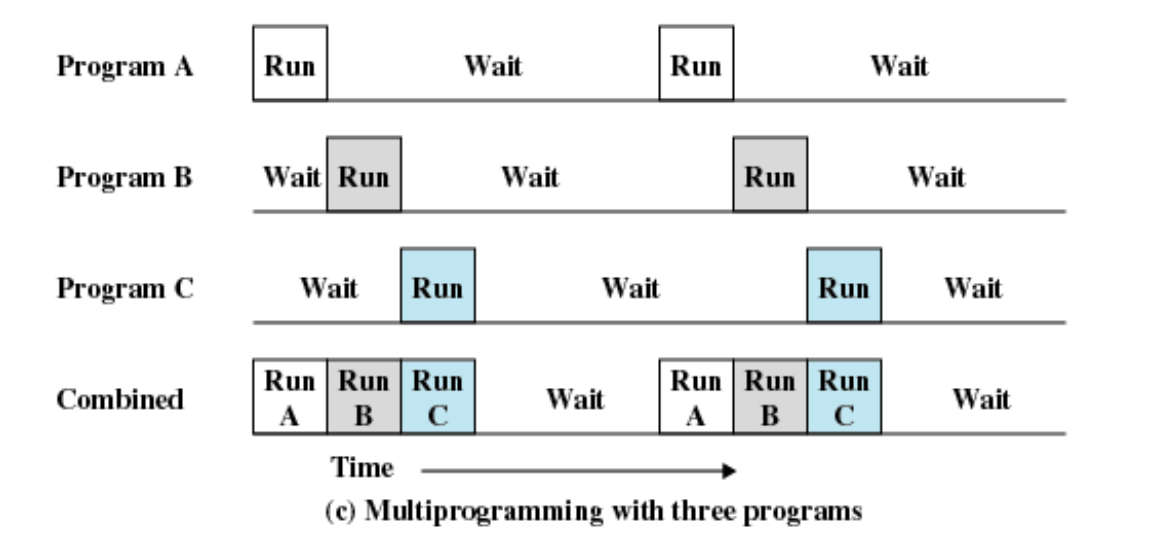
\includegraphics[width=1.00\textwidth]{Multi_programmazione}
	\end{figure}		
	La \textbf{difficoltà della multi-programmazione} sta nel gestire la memoria e scegliere quale processo mandare in esecuzione. \\
	Nella mono-programmazione un esempio può essere:
	\begin{itemize}
		\item Lettura di un record: 0.0015 sec;
		\item Esecuzione di 100 istruzioni: 0.0001 sec;
		\item Scrittura di un record: 0.0015 sec;
		\item Totale: 0.0031 sec
	\end{itemize}
	La percentuale di utilizzo della CPU è pari a $\dfrac{0.0001}{0.0031} = 0.032 = 3,2\%$ e notiamo quindi che è molto bassa.
	\section{I processi}
	Un processo può essere chiamato in diversi modi, come job o task e la definizione di processo è: \\
	{\centering \textbf{un'attività caratterizzata dall'esecuzione di una sequenza di istruzioni, uno stato corrente e un set di istruzioni di sistema.}} \\
	Le componenti di un processo sono:
	\begin{itemize}
		\item \textbf{programma}, cioè il codice eseguibile
		\item \textbf{Dati}
		\begin{itemize}
			\item variabili
			\item spazio di lavoro
			\item buffer
		\end{itemize}
		\item \textbf{Contesto di esecuzione}, cioè delle informazioni necessarie al SO per gestire il processo
		\begin{itemize}
			\item contenuto dei registri della CPU;
			\item priorità;
			\item stato di esecuzione;
			\item stato di attesa su un dispositivo I/O.
		\end{itemize}
	\end{itemize}
	\textbf{Implementazione di un processo}:
	\begin{figure}[H]
		\centering
		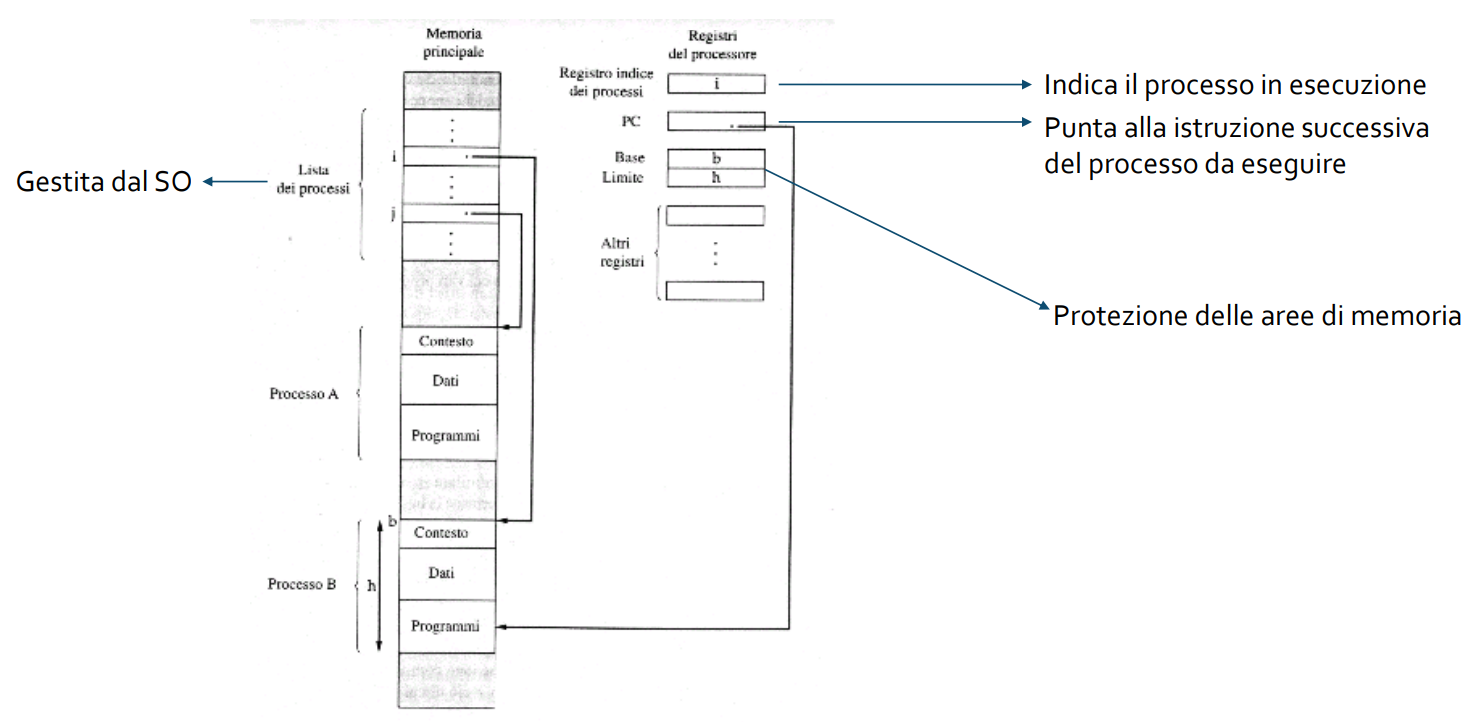
\includegraphics[width=1.00\textwidth]{implementazione_processo}
	\end{figure}
	\section{Gestione della memoria}
	Il sistema operativi deve compiere 5 compiti:
	\begin{enumerate}
		\item isolamento dei processi;
		\item allocazione e gestione automatica della memoria: la gerarchia delle memoria deve essere trasparente all'utente;
		\item supporto alla programmazione modulare: variazione di dimensione dei programmi
		\item protezione e controllo dell'accesso: gestione di aree di memoria condivise tra i processi;
		\item memorizzazione a lungo termine.
	\end{enumerate}
	Queste necessità sono soddisfatte da:
	\begin{itemize}
		\item \textbf{memoria virtuale:} i programmi indirizzano la memoria con riferimenti logici, ignorando quelli fisici e quando un programma è in esecuzione solo una sua parte risiede in memoria centrale;
		\item \textbf{file system:} implementa la memorizzazione a lungo termine.
	\end{itemize}
	\section{Stato e descrizione dei processi}
	Il compito principale del SO è quello di controllare l'esecuzione dei processi ed è possibile classificare lo stato attuale di un processo grazie, appunto, ad uno \textbf{stato}. In base allo stato di un processo questo viene gestito in maniera differente. \\
	Il SO, quindi, ha bisogno di uno strumento per gestire i processi che tenga conto delle informazioni relativi ad essi. \\
	Questo prende il nome di \textbf{Descrittore di un processo}, oppure \textbf{PCB}, Process Control Block. \\
	Il Process Control Block è composto da:
	\begin{itemize}
		\item \textbf{Identificatore del processo}, un PID, Process Identification, che si tratta di un valore numerico;
		\item \textbf{Info sullo stato del processore}
		\begin{itemize}
			\item Registri dati visibili all'utente che dipendono dall'architettura del calcolatore;
			\item Registri di controllo e di stato:
			\begin{itemize}
				\item Program Counter, PC e contiene l'indirizzo della prossima istruzione da eseguire;
				\item Registri di stato che includono i flag per l'abilitazione degli interrupt;
				\item Registri che contengono codici relativi alla condizione come segno, overflow ecc.
			\end{itemize}
			\item Puntatori allo stack che viene usato per procedure e funzioni
		\end{itemize}
		\item \textbf{Informazioni di controllo del processo}
			\begin{itemize}
				\item Schedulazione e informazioni di stato
				\begin{itemize}
					\item stato del processo;
					\item priorità nelle code di scheduling;
					\item informazioni correlate alla schedulazione, come tempo di attesa, tempo di esecuzione ecc.;
					\item se in attesa, l'evento per il quale è in attesa.
				\end{itemize}
				\item Strutturazione dati: puntatori ad altri processi
				\item Comunicazione tra processi: flag, segnali e messaggi per la comunicazione
				\item Privilegi in relazione all'uso della memoria, dei dispositivi ecc.
				\item Gestione della memoria, cioè i limiti di memoria e gli indirizzi accessibili
				\item Contabilizzazione delle risorse cioè le risorse controllate dal processo, come i dispositivi I/O, i file aperti ecc, e la loro storia
			\end{itemize}
	\end{itemize}
	\section{Creazione e terminazione dei processi}
	Gli eventi che portano alla \textbf{creazione} dei processi possono essere:
	\begin{itemize}
		\item richiesta dal terminale, cioè un utente accede al sistema
		\item il SO genera un processo sulla base della richiesta di un processo utente come ad esempio la stampa
		\item un processo utente genera un nuovo processo
	\end{itemize}
	Gli eventi che portano alla \textbf{terminazione} dei processi possono essere:
	\begin{itemize}
		\item terminazione normale;
		\item uscita dell'utente dall'applicazione;
		\item superamento del tempo massimo;
		\item memoria non disponibile;
		\item violazione dei limiti di memoria;
		\item fallimento di un'operazione;
		\item terminazione del genitore;
		\item richiesta del genitore.
	\end{itemize}
	\section{Modello a 2 stati}
	\begin{figure}[H]
		\centering
		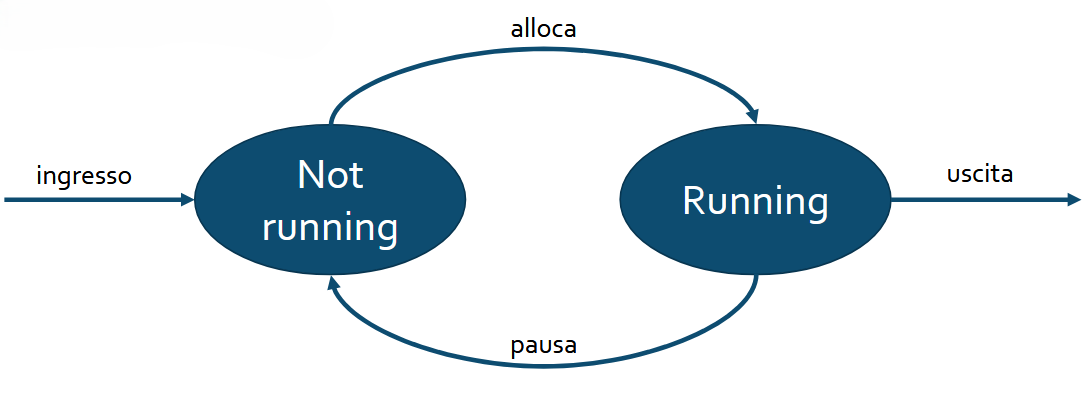
\includegraphics[width=0.6\textwidth]{modello_2_stati}
	\end{figure}
	Il modello a 2 stati è composto dagli stati di:
	\begin{itemize}
		\item \textit{Running}, dove il processo sta eseguendo le istruzioni e sta utilizzando attivamente la CPU;
		\item \textit{Not Running}, questo stato include due possibilità:
		\begin{itemize}
			\item il processo è pronto per essere eseguito;
			\item il processo è in attesa di un evento o di un dispositivo I/O.
		\end{itemize}
	\end{itemize}
	Lo scheduler non può scegliere il processo da più tempo in attesa in quanto potrebbe essere in attesa di un trasferimento I/O.
	
	\section{Modello a 5 stati}
	Dal modello a 2 stati si passa al modello 5 stati:
	\begin{itemize}
		\item vengono introdotti gli stati \textit{New} e \textit{Exit} o \textit{Terminated};
		\item lo stato di \textit{Not Running} viene diviso negli stati di \textit{Ready}, cioè pronto per l'esecuzione e \textit{Blocked} cioè in attesa di un evento, di una risorsa o altro.
	\end{itemize}
	\begin{figure}[H]
		\centering
		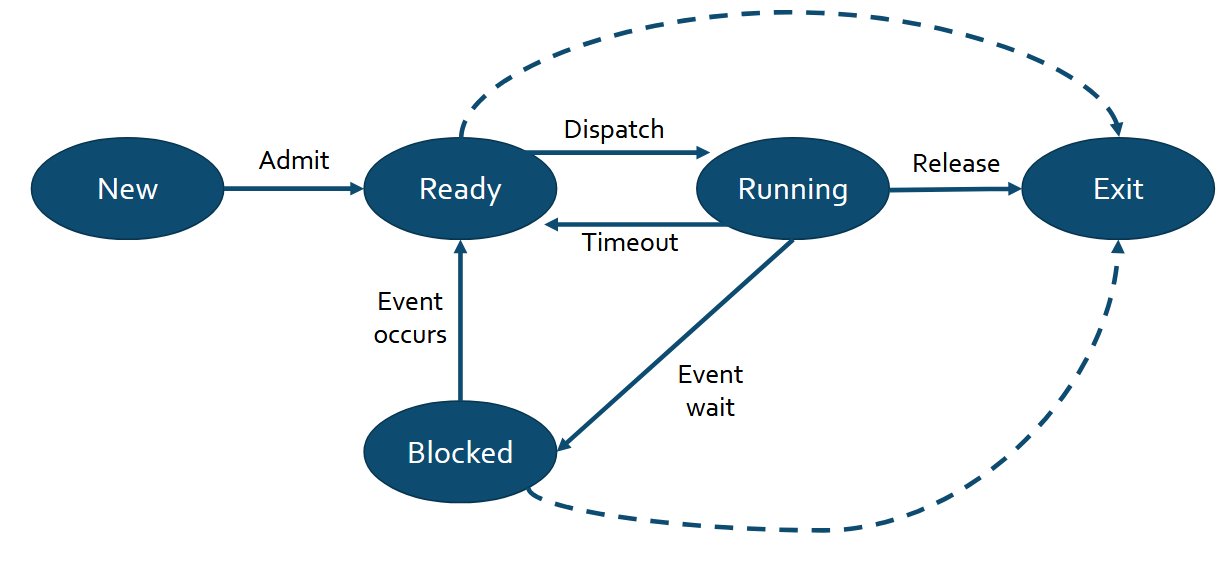
\includegraphics[width=0.7\textwidth]{modello_5_stati}
	\end{figure}
	Lo stato di \textit{New} associa il PID, alloca e costruisce le tabelle per la gestione del processo ma non viene caricato in memoria. \\
	Lo stato di \textit{Exit} rilascia le risorse detenute dal processo e mantiene alcune informazioni, come le risorse utilizzate, utile per la contabilità. \\
	Un processo può uscire dallo stato di \textit{Running} per diversi motivi:
	\begin{itemize}
		\item è in attesa di un evento e quindi passa nello stato di \textit{Blocked};
		\item termina il tempo di esecuzione associato ad esso e passa nello stato di \textit{Ready}.
	\end{itemize}
	\section{Context switch}
	Il Context Switch riguarda il passaggio della CPU ad un nuovo processo e le cause possono essere:
	\begin{itemize}
		\item \textbf{Clock interrupt}, il processo ha terminato il tempo a sua disposizione e torna nella coda di ready
		\item \textbf{I/O interrupt}, un'operazione di I/O è terminata e il SO sposta il processo da blocked a ready e decide se riprendere l'esecuzione del processo precedente;
		\item \textbf{Memory fault}, l'indirizzo di memoria generato è sul disco e deve essere portato in RAM. Il SO carica il blocco, il processo che ha generato la richiesta è in blocked e al termine del trasferimento andrà in ready;
		\item \textbf{Trap}, errore di esecuzione e il processo potrebbe anche andare in exit;
		\item \textbf{Supervisor call}
	\end{itemize}
	Le operazioni svolte dal SO in modalità supervisor al momento del cambio del processo in stato di running sono:
	\begin{itemize}
		\item salvataggio del PCB del processo che abbandona la CPU;
		\item cambio di valore di stato nel PCB del processo, quindi da running può passare a blocked, ready o exit;
		\item Spostamento del PCB in nuova coda come ready o blocked, o deallocare le risorse in caso di exit;
		\item Aggiornamento delle strutture dati gestione memoria
		\item Selezione di un nuovo processo per lo stato di running;
		\item Aggiornamento del suo stato nel PCB;
		\item Ripristino del contesto.
	\end{itemize}
	Il context switch time è overhead cioè il sistema non svolge nessun compito utile all'utente e il tempo dipende dalla complessità del SO e dell'hardware.
	\section{Modalità di esecuzione dei processi}
	\noindent
	\textbf{Modalità utente:} esecuzione di processi utente
	
	\noindent
	\textbf{Modalità Sistema o Kernel o Controllo:} esecuzione di istruzioni che hanno come scopo
	
	\begin{itemize}[leftmargin=*, itemsep=0.2em]
		\item \textbf{Gestione dei Processi}
		\begin{itemize}[leftmargin=2em, itemsep=0.1em]
			\item Creazione e terminazione
			\item Schedulazione
			\item Cambio di contesto
			\item Sincronizzazione
			\item PCB
		\end{itemize}
		
		\item \textbf{Gestione della Memoria}
		\begin{itemize}[leftmargin=2em, itemsep=0.1em]
			\item Allocazione
			\item Trasferimento disco/RAM e viceversa
			\item Gestione della paginazione, segmentazione...
		\end{itemize}
		
		\item \textbf{Gestione I/O}
		\begin{itemize}[leftmargin=2em, itemsep=0.1em]
			\item Gestione buffer
			\item Allocazione canali I/O
		\end{itemize}
		
		\item \textbf{Supporto}
		\begin{itemize}[leftmargin=2em, itemsep=0.1em]
			\item Gestione interruzioni
			\item Contabilità
		\end{itemize}
	\end{itemize}
	\section{Creazione dei processi}
	\begin{enumerate}[leftmargin=*, itemsep=0.5em]
		\item Assegnare al processo un PID unico; aggiungere una entry level alla tabella dei processi
		
		\item Allocare lo spazio per il processo e per tutti gli elementi della sua immagine (PCB, User Stack, area di memoria dati e istruzioni, aree condivise)
		
		\item Inizializzazione del PCB
		\begin{itemize}[leftmargin=2em, itemsep=0.1em]
			\item Stato del processore = 0
			\item PC = prossima istruzione
			\item Puntatori allo stack
			\item Stato = ready
		\end{itemize}
		
		\item Inserimenti nella coda di ready
		
		\item Estende le strutture al fine della fatturazione o delle statistiche
	\end{enumerate}
	
	\section{Modello a 6 stati}
	Dal modello a 5 stati si è passati al modello a 6 stati dove viene introdotto lo stato di \textit{Suspend}. \\
	Questo stato è stato introdotto in quanto con molta probabilità tutti i processi rimangono in attesa di eventi I/O e per questo è inefficiente tenere tutti i processi in attesa di un evento in memoria RAM e quindi, con lo stato di \textit{Suspend} i processi in attesa di un evento vengono trasferiti dalla memoria RAM alla memoria secondaria, che è un'altra operazione di I/O ma è molto rapida. \\
	Un'altra soluzione sarebbe quella di espandere la memoria ma è inefficiente in quanto costoso e perchè i programmi diventano sempre più grandi.
	\begin{figure}[H]
		\centering
		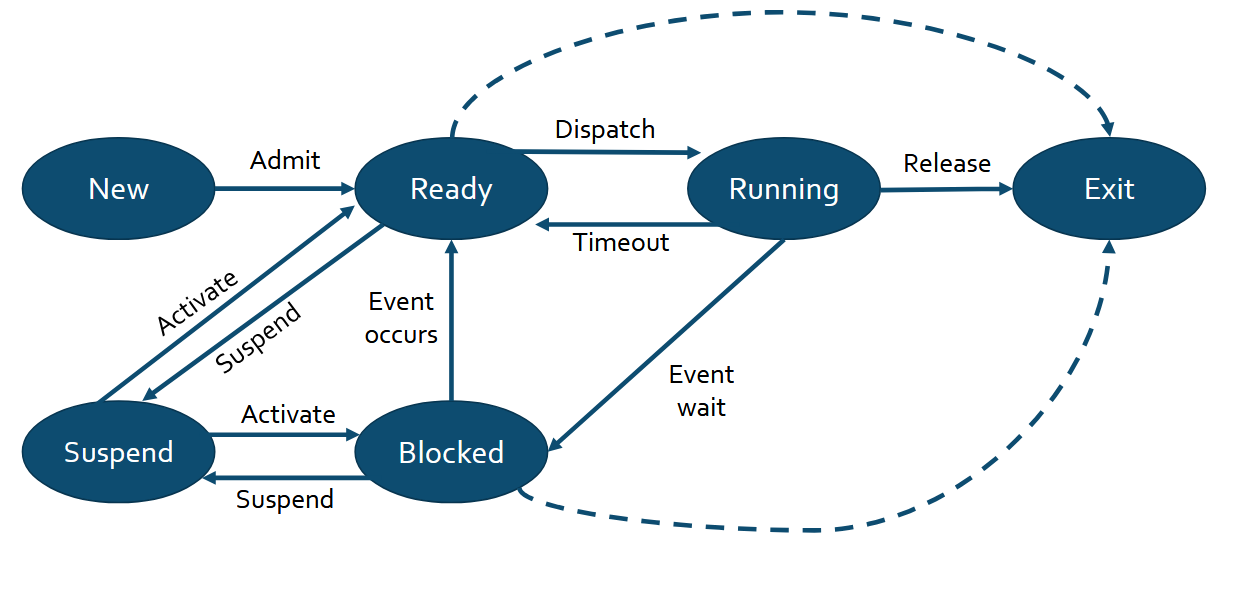
\includegraphics[width=0.7\textwidth]{modello_6_stati}
	\end{figure}
	Il modello a 6 stati prevede due operazioni:
	\begin{enumerate}
		\item \textit{Swap out}, la transizione del processo da \textit{Blocked} a \textit{Suspend} e quindi il passaggio dalla memoria RAM alla memoria secondaria;
		\item \textit{Swap in}, ovvero la transizione del processo da \textit{Suspend} a \textit{Blocked} o  \textit{Ready} e quindi il passaggio dalla memoria secondaria alla memoria RAM.
	\end{enumerate}
	Il modello a 6 stati pone lo stesso problema del modello a 2 stati, cioè non si può semplicemente caricare dalla memoria il processo da più tempo in attesa in quanto potrebbe ancora star aspettando che la risorsa necessaria si liberi o potrebbe ancora essere in attesa che l'evento desiderato si verifichi. \\
	Pertanto si è passati al modello a 7 stati.
	\section{Modello a 7 stati}
	Nel modello a 7 stati, lo stato di \textit{Suspended} viene suddiviso in due ulteriori stati:
	\begin{itemize}
		\item \textit{Ready/Suspended} dove si trovano i processi in memoria secondaria ma pronti per passare in memoria RAM e per essere eseguiti;
		\item \textit{Blocked/Suspended} dove si trovano i processi in memoria secondaria ancora in attesa che l'evento desiderato si verifichi o che la risorsa necessaria all'esecuzione diventi libera.
	\end{itemize}
	\begin{figure}[H]
		\centering
		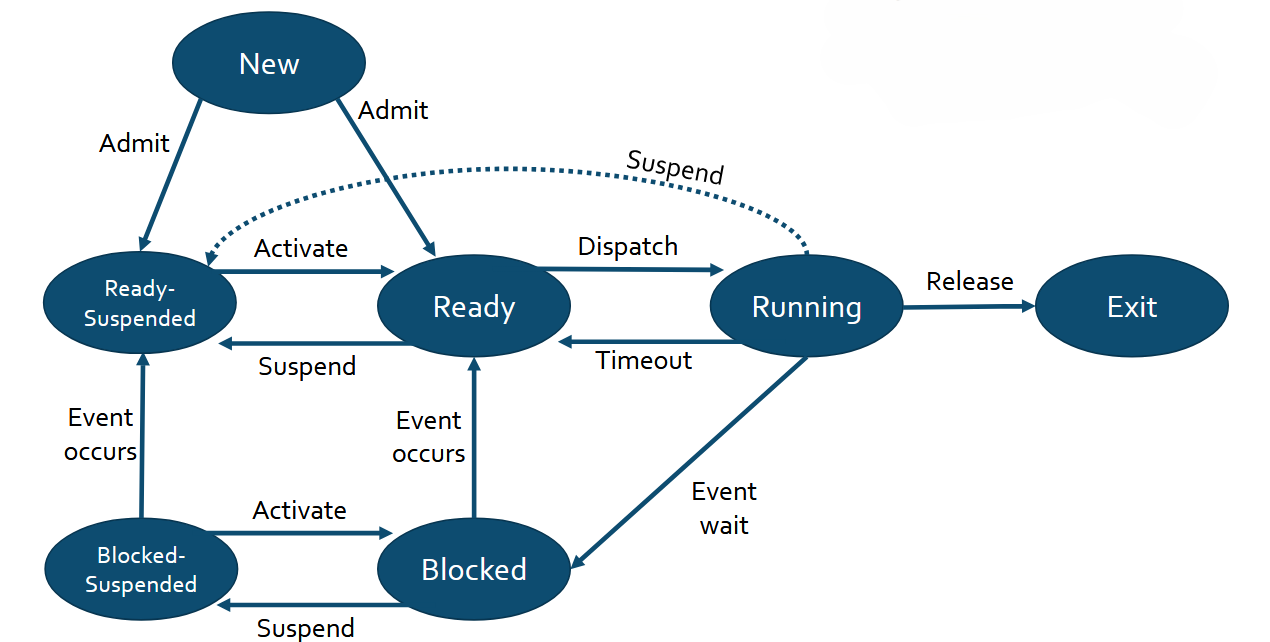
\includegraphics[width=0.8\textwidth]{modello_7_stati}
	\end{figure}
	\section{Schedulazione}
	La schedulazione, cioè la scelta dell'ordine di esecuzione dei processi, e la relativa politica di allocazione deve tenere in conto:
	\begin{itemize}
		\item \textbf{equità:} cioè tutti i processi appartenenti ad una stessa classe o con richieste simili o stesso costo devono avere la stessa possibilità di accesso alla risorsa;
		\item \textbf{tempo di risposta differenziale}: il SO discrimina tra classi che hanno bisogno di risorse diverse e di tempi diversi, ad esempio i processi I/O bound vengono schedulati per prima;
		\item \textbf{Efficienza:} massimizzare il throughput, cioè la quantità di dati trasmessi e minimizzare il tempo di risposta
	\end{itemize}
	Lo \textbf{scheduling} è insieme di tecniche e meccanismi interni del SO che amministrano l'ordine in cui il lavoro viene svolto e l'\textbf{obiettivo primario} dello scheduling è l'ottimizzazione delle prestazioni del sistema. \\
	Il SO può prevedere fino a 3 tipi di scheduler:
	\begin{itemize}
		\item \textbf{Scheduler di lungo termine}, questo determina quali programmi sono ammessi nel sistema per essere processati cioè dallo stato di new allo stato di ready o ready-suspended. Il lavoro dell'SLT è quello di stimare il comportamento globale dei job in base a stime effettuate dal programmatore o dal sistema che forniscono informazioni sulle risorse necessarie, dimensione della memoria, tempo di esecuzione ecc. \\
		Le \textbf{strategie} principali dello scheduler di lungo termine sono: 
		\begin{enumerate}
			\item fornire alla coda dei processi pronti gruppi di processi che siano bilanciati tra loro nello sfruttamento della CPU e dell'I/O;
			\item aumentare il numero di processi provenienti dalla coda batch, quando il carico della CPU diminuisce;
			\item diminuire, fino anche a bloccare, i lavori provenienti dalla coda batch, quando il carico aumento e i tempi di risposta del sistema diminuiscono.
		\end{enumerate}
		La frequenza di chiamata dell'SLT è bassa e consente di implementare strategie complesse di selezione dei lavori e di dimensionamento del carico dei processi di inviare alla coda pronti.
		\item \textbf{Scheduler di medio termine}, questo si occupa di gestire la schedulazione delle transizioni da ready-suspended a ready e da blocked-suspended a blocked, quindi si occupa di trasferire i processi dalla memoria secondaria alla memoria centrale e viene attivato quando si rende disponibile lo spazio in memoria e quando l'arrivo di processi pronti scende al di sotto di una certa soglia specificata. \\
		La presenza di molti processi sospesi in memoria riduce la possibilità per nuovi processi pronti e in questo caso lo SBT è obbligato a scegliere trami pochi processi pronti.
		\begin{itemize}
			\item Utilizza le informazioni del PCB per stabilire la richiesta di memoria del processo;
			\item tenta di allocare spazio in memoria centrale;
			\item riposiziona il processo in memoria nella coda dei pronti.			
		\end{itemize}
		\item \textbf{Scheduler di breve termine} o anche detto \textbf{dispatcher} gestisce la transizione da ready a run e viene eseguito molto frequentemente e la sua \textbf{strategia} è quella di massimizzare le prestazioni del sistema secondo un specifico insieme di obiettivi. \\
		Questo viene invocato quando si verifica un evento: 
		\begin{itemize}
			\item clock interrupt;
			\item I/O interrupt;
			\item chiamate del SO;
			\item signals.
		\end{itemize}
	\end{itemize}
	\subsection{Scheduling della CPU nel dispatcher}
	\begin{figure}[H]
		\centering
		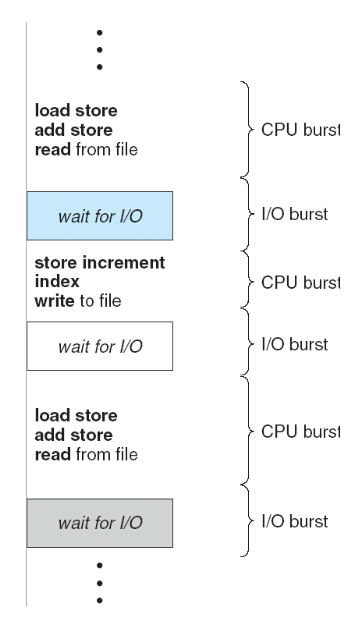
\includegraphics[width=0.7\textwidth]{scheduling_CPU_dispatcher}
	\end{figure}
	Lo scheduling della CPU riguarda la distribuzione delle sequenze di elaborazione della CPU e un processo durante la sua fase di esecuzione si può trovare in due stati:
	\begin{enumerate}
		\item Si trova nel suo ciclo di elaborazione e quindi sta utilizzando attivamente la CPU;
		\item Si trova in attesa di un'operazione di I/O		
	\end{enumerate}
	Inoltre, i processi possono essere divisi in due macrocategorie:
	\begin{itemize}
		\item Processi \textbf{CPU bound} e sono processi che presentano poche operazioni di I/O  e quindi sono più veloci;
		\item Processi \textbf{I/O bound} e sono processi che presentano molte operazioni di I/O e sono più lenti rispetto ai CPU bound.
	\end{itemize}
	\subsection{Algoritmi di schedulazione}
	Definiamo due cose:
	\begin{enumerate}
		\item il \textbf{tempo di ricircolo} che rappresenta il tempo trascorso tra l'avvio di un processo, cioè la sua immissione nel sistema e la terminazione di esso;
		\item il \textbf{tempo di attesa} cioè il tempo che un processo trascorre in attesa delle risorse. Si può calcolare come differenza tra il tempo di ricircolo e il tempo di esecuzione e quindi, valuta la sorgente di inefficienza che è il prezzo da pagare per condividere le risorse.
	\end{enumerate}
	L'efficienza degli algoritmi di scheduling è misurabile utilizzando questi 2 tempi e un buon algoritmo di scheduling bilancia l'esecuzione dei processi al meglio, massimizzando l'uso del processore e riducendo i tempi di attesa. \\
	Gli algoritmi possono avere 2 politiche:
	\begin{itemize}
		\item \textbf{non preemptive}, cioè non interrompibile e un processo in running abbandonerà questo stato solo se termina l'esecuzione o si blocca per un'operazione di I/O;
		\item \textbf{preemptive}, cioè interrompibile e un processo in running può essere interrotto e spostato in ready dal SO, e questo fa si che nessun processo può monopolizzare il processore, d'altra parte, però, crea dei problemi se ci sono dei processi che condividono dati e richiedono meccanismi di sincronizzazione
	\end{itemize}
	\subsubsection{FCFS - First Come First Served}
	\begin{figure}[H]
		\centering
		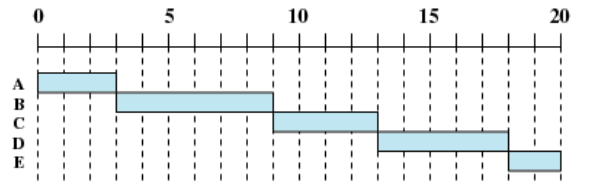
\includegraphics[width=0.6\textwidth]{FCFS}
	\end{figure}
	Nell'algoritmo FCFS si applica il principio della coda, ovvero ogni processo entra nella coda nello stato di \textit{Ready} e quando un processo abbandona lo stato di \textit{Running} si sceglie il processo che è da più tempo residente nello stato di \textit{Ready}. \\
	Questo algoritmo favorisce i processi CPU bound in quanto i processi I/O bound, che richiedono poco tempo di esecuzione, potrebbero attendere molto tempo prima che gli venga assegnata la CPU e quindi si genera l'effetto convoglio dove tutti i processi in coda aspettano che un processo CPU bound termini. \\
	In questo algoritmo, quindi, le risorse del sistema non vengono sfruttate a pieno.
	\subsubsection{Algoritmo Event Driven}
	Questo algoritmo presenta uno schema che ragiona secondo un \textbf{valore di priorità} assegnato a ciascun processo e lo scheduler sceglierà semplicemente il processo pronto con priorità maggiore. \\
	La priorità può essere assegnata dall'utente o dal sistema e può essere di tipo statico o dinamico. La priorità dinamica varia in base a:
	\begin{itemize}
		\item valore iniziale;
		\item caratteristiche del processo;
		\item richiesta di risorse;
		\item comportamento durante l'esecuzione.
	\end{itemize}  
	Questo algoritmo viene applicato nei sistemi dove il tempo di risposta, soprattutto ad eventi esterni, è critico. \\
	Il sistemista può influire sull'ordine di esecuzione dei processi modificando le priorità assegnate ad essi e le prestazioni del sistema sono dipese dalla scelta delle priorità assegnate a ciascun processo. \\
	Le priorità sono definite:
	\begin{itemize}
		\item esternamente al SO in base alla rilevanza del processo e alla sua criticità;
		\item internamente al SO utilizzando grandezze misurabili come l'uso della memoria, i file aperti e il rapporto tra picchi medi di I/O o CPU.
	\end{itemize}
	Questo algoritmo non è in grado di garantire il completamento di un processo in un intervallo di tempo finito dalla sua creazione, in quanto potrebbe essere continuamente sorpassato da processi a priorità più alta causando quindi la \textbf{starvation}. \\
	La soluzione a questo problema è data dalla tecnica dell'\textbf{aging}, dove al passare del tempo di un processo in \textit{Ready} la priorità del processo aumenta.
	\subsubsection{Algoritmo Round Robin - RR}
	Questo algoritmo utilizza il principio del \textbf{time slice} ovvero una preemption basata sul clock. Ogni processo utilizza il processore per un dato intervallo di tempo e al verificarsi di un interrupt il processo in esecuzione passa nello stato di \textit{Ready}. \\
	Con $n$ processi in \textit{Ready} e un tempo $q$ assegnatogli, ogni processo ottiene $\dfrac{1}{n}$ del tempo di CPU in frazioni di tempo al più pari a $q$ e il tempo massimo di attesa è di $(n-1)q$. \\
	Le prestazioni dipendono dal quanto tempo assegnato perchè se la $q$ è molto grande allora si degenera in un FCFS mentre se è troppo piccolo c'è un numero elevato di context switch e quindi si consumano molte risorse. \\
	Questo algoritmo fornisce una buona condivisione delle risorse del sistema:
	\begin{itemize}
		\item i processi più brevi possono completare le loro operazioni in un buon $q$;
		\item i processi più lunghi sono forzati a passare più volte per la coda dei processi pronti;
		\item per i processi interattivi lunghi, se l'esecuzione riesce a completarsi in un $q$, il tempo di risposta è buono.
	\end{itemize}
	La realizzazione di un RR richiede il supporto di un Timer che invia un'interruzione ad ogni scadenza di $q$.
	\subsubsection{Highest Response Ratio Next - HRRN}
	Definiamo due variabili:
	\begin{itemize}
		\item $w$ il tempo speso nella coda di \textit{Ready};
		\item $s$ il tempo di servizio previsto.
	\end{itemize}
	Si definisce il Response Ratio come:
	\[
	RR = \frac{w + s}{s}
	\] 
	Questo algoritmo manda in esecuzione il processo con il più alto valore di RR e quando un processo entra nella coda di \textit{Ready} per la prima volta ha un RR = 1 e al passare del tempo nella coda di \textit{Ready} il valore del Response Ratio aumenta e quindi viene implementa la tecnica dell'aging.
	\subsubsection{Shortest Process Next - SPN}
	In questo algoritmo, il processo scelto dalla coda di \textit{Ready} è quello con il più breve tempo di esecuzione stimato. \\
	Questo algoritmo è ottimale nel senso che fornisce il tempo media di attesa minimo ma è difficile stimare la durata della prossima sequenza di CPU ed è possibile che si verifichi la starvation per processi fortemente CPU bound. \\
	Questo algoritmo ha una versione preemptive dove se arriva un processo con una sequenza di CPU minore rispetto al processo attualmente in esecuzione si ha il rilascio della CPU a favore del processo appena arrivato. Questo schema viene chiamato \textit{Shortest Remaining Time First (SRTF)} oppure \textit{Shortest Remaining Time Next (SRTN)}.
	\subsubsection{Schedulazione a code multiple}
	In questo schema la coda di Ready viene divisa in sotto-code:
	\begin{itemize}
		\item Foreground per i processi interattivi;
		\item Background per i processi batch
	\end{itemize}
	e ogni coda ha il proprio algoritmo di schedulazione ma è necessario uno scheduling fra le code che può essere:
	\begin{itemize}
		\item A priorità fissa e con prelazione, ad esempio serve prima la Foreground e poi la Background;
		\item Time slice dove ad ogni coda è associato un quanto di tempo di utilizzo della CPU.
	\end{itemize}
	È possibile un'ulteriore soluzione, quella della \textbf{Schedulazione a code multiple con feedback} dove viene implementata la tecnica dell'aging dove un processo può essere spostato da una coda all'altra. 
 	\chapter{Thread}
	Un thread è un \textbf{flusso di esecuzione indipendente, una traccia,} all'interno di un processo. \\
	Le motivazioni per le quali solitamente un processo viene diviso in più thread sono:
	\begin{itemize}
		\item ottenere un parallelismo dei flussi di esecuzione all'interno del processo;
		\item gestire chiamate bloccanti o situazioni di risposta asincrona.
	\end{itemize}
	Ad esempio se dobbiamo implementare un web server, se questo fosse implementato come un monothread potremmo gestire solo un client alla volta e le altre richieste verrebbero ignorate e quindi ci sono due soluzioni possibili per risolvere questa situazione, cioè di implementare il server come un processo che resta in attesa delle richieste e poi scegliere se avviare un nuovo processo che processi la singola richiesta o avviare un thread che processi la singola richiesta. \\
	Ovviamente, avviare ed effettuare un context switching di un thread è meno oneroso di avviare un processo.
	\section{Differenza tra thread e processi}
	Un \textbf{processo} possiede delle risorse:
	\begin{itemize}
		\item ha uno spazio di indirizzamento virtuale che contiene l'immagine del processo; 
		\item può richiedere ulteriore memoria;
		\item può chiedere il controllo di canali di I/O; 
		\item può chiedere il controllo di dispositivi;
		\item può chiedere files.
	\end{itemize}
	Il processo inoltre ha un'unità di esecuzione, quindi ha uno stato, una priorità e deve essere schedulato, tutte queste informazioni sono contenute nel PCB. \\
	Un \textbf{thread} non ha risorse perchè utilizza quelle del processo e per questo viene anche chiamato \textbf{Light Weigth Process (LWP)}. \\
	Un thread ha un proprio stato, una propria priorità e deve essere schedulato, ma tra i thread e sottostando alla schedulazione del processo. Tutte queste informazioni sono contenute nel \textbf{Thread Control Block (TCB)}.
	\section{Multithreading}
	\textbf{Il multithreading è la capacità di un Sistema Operativo di supportare più thread per ogni processo.} \\
	Le diverse possibilità sono:
	\begin{itemize}
		\item \textbf{singolo processo a singolo thread}, come MS-DOS dove il thread esiste nel processo;
		\item \textbf{singolo processo e thread multipli};
		\item \textbf{processi multipli a singolo thread}, come UNIX;
		\item \textbf{Multithread, più processi con più thread}, come Windows, MAC, Solaris ecc.
	\end{itemize}
	Sappiamo che un thread condivide le risorse del processo e in un sistema multithreading, i thread: 
	\begin{itemize}
		\item condividono lo stato e le risorse del processo a cui appartengono;
		\item risiedono nello stesso spazio di indirizzamento,
		\item hanno accesso agli stati.
	\end{itemize}
	Dunque visto che i thread condividono tutti gli stessi dati è più facile scambiarsi informazioni.
	\section{Vantaggi e problemi dei thread}
	I thread presentano alcuni vantaggi:
	\begin{itemize}
		\item il \textbf{tempo di creazione} di un nuovo thread è minore del tempo di creazione di un nuovo processo;
		\item il \textbf{tempo di terminazione} di un thread è minore del tempo di terminazione di un processo;
		\item il \textbf{tempo di context switching} tra thread all'interno dello stesso processo è minore del tempo di context switching tra processi;
		\item i thread all'interno di uno stesso processo condividono memoria e files quindi c'è uno scambio dati senza richiedere l'intervento del kernel ma c'è la necessità di sincronizzare i thread nel momento in cui devono accedere alla stessa risorsa del processo.
	\end{itemize}
	Però, se un processo viene sospeso questo comporta la sospensione di tutti i thread contemporaneamente perchè si deve liberare spazio in memoria e i thread utilizzano lo stessso spazio di memoria condivisa. Inoltre, la terminazione di un processo richiede che tutti i thread siano terminati.
	\section{Stati dei thread}
	Gli stati dei thread, a differenza di quelli dei processi, sono solo 3: 
	\begin{itemize}
		\item Ready;
		\item Running;
		\item Blocked.
	\end{itemize}
	Lo stato di suspended non c'è perchè non ha senso, in quanto se un processo viene swappato, di conseguenza anche i trhead a esso collegati vengono swappati.
	\section{Operazioni di base}
	Le operazioni che si possono effettuare su un thread sono:
	\begin{itemize}
		\item \textbf{Creazione}: quando viene creato un processo viene creato un thread e un thread può creare altri thread;
		\item \textbf{Blocco} a causa di un attesa di un evento e avviene il salvataggio del contesto per il thread;
		\item \textbf{Sblocco}: lo stato nel TCB viene modificato da blocked a ready e il thread viene accodato a quelli in attesa di processore;
		\item \textbf{Terminazione}: avviene la deallocazione del contesto registri e la deallocazione dello stack.
	\end{itemize}
	\section{Esempi di multithreading}
	Il \textbf{Remote Procedure Call (RPC)} è la chiamata da parte di un processo a una procedura attiva su un elaboratore diverso dal chiamante. \\
	\begin{figure}[H]
		\centering
		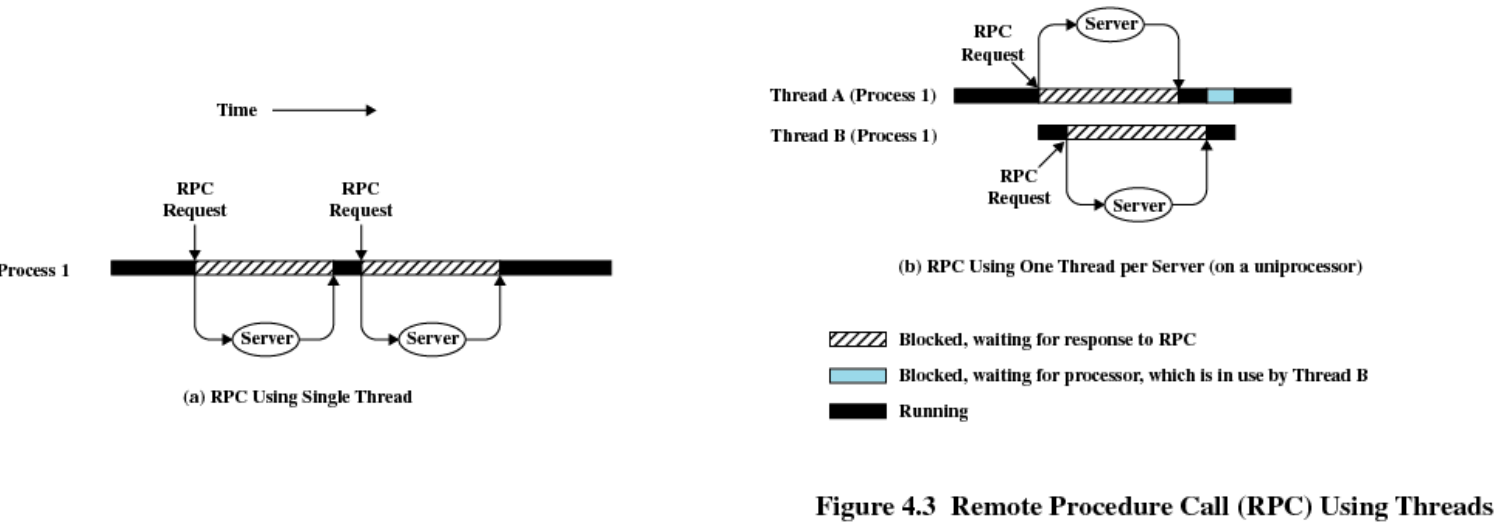
\includegraphics[width=1.00\textwidth]{RPC}
	\end{figure}
	Vediamo un esempio di multithreading: un programma di video-scrittura, gestione e pubblicazione di pagine su desktop. \\
	Ci sono tre thread sempre attivi: 
	\begin{enumerate}
		\item Gestione degli eventi;
		\item Gestione dei servizi come stampa, lettura dati, disposizione testo e attivazione di altri thread;
		\item Disegno dello schermo.
	\end{enumerate}
	\begin{figure}[H]
		\centering
		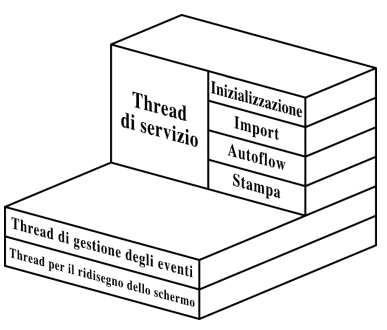
\includegraphics[width=1.00\textwidth]{mulithreading}
	\end{figure}
	Un altro esempio può essere lo scorrimento della pagina con barra laterale: qui abbiamo un thread eventi che controlla la barra di scorrimento e un thread di ridisegno dello schermo che ridisegna la pagina in base allo scorrimento. In questo esempio è necessario che i due thread siano sincronizzati.
	\section{Categorie di threaed}
	Esistono due tipologie di thread:
	\begin{itemize}
		\item \textbf{User Level Thread (ULT)}
		\begin{itemize}
			\item \textbf{Realizzati tramite librerie senza l'intervento del kernel}
			\item \textbf{Trasparenti al kernel}
		\end{itemize}
		Lo svantaggio è che se il kernel è a singolo thread il blocco del thread blocca l'intero processo, ma il sistema operativo continua comunque a schedulare i processi,
		\item \textbf{Kernel Level Thread (KLT)}
		\begin{itemize}
			\item \textbf{il kernel si occupa della creazione, scheduling e gestione};
			\item \textbf{possono essere eseguiti su diversi processori};
		\end{itemize}
		Questa tipologia di thread hanno una gestione più lenta degli ULT.
	\end{itemize}
	\subsection{User Level Thread}
	Come abbiamo detto questi thread sono realizzati tramite delle libreria senza l'intervento da parte del kernel quindi il lavoro di gestione dei threads è svolto dalla libreria utente e il kernel ignora la loro esistenza. Il modello di questi thread è \textbf{molti a uno}. \\
	La libreria permette:
	\begin{itemize}
		\item creazione e distruzione dei threads;
		\item scambio messaggi tra threads;
		\item schedulazione;
		\item salvataggio e caricamento dei contesti dei thread.
	\end{itemize}
	Bisogna ricordare che tutte queste attività vengono \textbf{svolte all'interno del processo utente}, quindi il \textbf{kernel continua a schedulare i processi come unità a se stanti.}
	\begin{figure}[H]
		\centering
		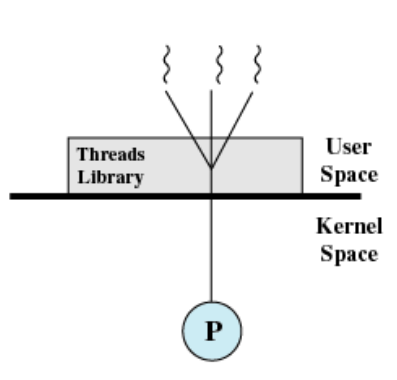
\includegraphics[width=0.50\textwidth]{ULT}
	\end{figure}
	\paragraph{Vantaggi e svantaggi}
	I \textbf{vantaggi} dei thread ULT sono:
	\begin{itemize}
		\item \textbf{risparmio di sovraccarico}, in quanto il cambio di thread avviene all'interno dello spazio di indirizzamento utente e non viene richiesto l'intervento del kernel;
		\item \textbf{Schedulazione diversa per ogni applicazione}: questi thread sono ottimizzati in base al tipo di applicazione;
		\item \textbf{ULT eseguito da qualsiasi sistema operativo}.
	\end{itemize}
	Gli \textbf{svantaggi} dei thread ULT sono:
	\begin{itemize}
		\item \textbf{la chiamata a sistema da parte di un thread blocca tutti i thread del processo};
		\item \textbf{il kernel assegna un processo ad un singolo processore quindi non si può avere multiprocessing a livello di thread}, cioè thread dello stesso processo su più processori. \\
		Esistono delle soluzioni parziali a questi problemi che sono:
		\begin{itemize}
			\item sviluppo dell'applicazione a livello di processi ma andremmo a perdere tutti i vantaggi dei thread;
			\item \textbf{jacketing:} conversione di una chiamata bloccante in una non bloccante, ad esempio nel caso di I/O si invoca una procedura di jacketing che verifica se il dispositivo è occupato, in caso affermativo il thread passa in ready e un altro thread va in run.
		\end{itemize}
	\end{itemize}
	\subsection{Kernel Level Thread}
	Per quanto riguarda i kernel level thread il lavoro di gestione dei threads è svolto dal kernel e il \textbf{modello è uno a uno}. 
	\begin{figure}[H]
		\centering
		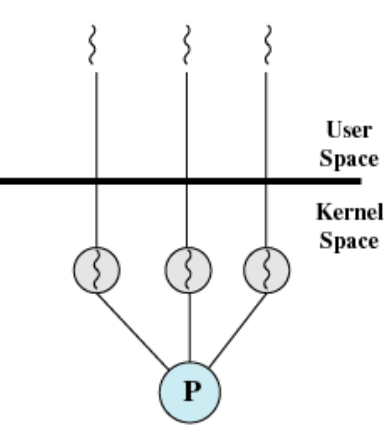
\includegraphics[width=0.5\textwidth]{KLT}
	\end{figure}
	A livello utente, c'è una API che consente l'accesso alla parte del kernel che gestisce i thread, i compiti del kernel sono:
	\begin{itemize}
		\item mantenere info sul contesto del processo;
		\item mantenere info sul contesto dei thread;
		\item mantenere info sullo scambio dei messaggi tra threads.
	\end{itemize}
	La \textbf{schedulazione} per questa tipologia di thread viene \textbf{effettuata a livello di thread}
	\begin{itemize}
		\item se un thread di un processo è bloccato, un altro thread dello stesso processo può essere eseguito;
		\item threads di uno stesso processo possono essere schedulati sy diversi processori.
	\end{itemize}
	Lo \textbf{svantaggio} dei kernel level thread è l'\textbf{overhead} perchè il trasferimento del controllo da un thread a un altro richiede l'intervento del kernel.
	\subsection{Approcci misti}
	Esiste un altro tipo di modello, il \textbf{modello molti a molti}, cioè più thread di livello utente sono in corrispondenza con più thread di livello kernel.
	\begin{figure}[H]
		\centering
		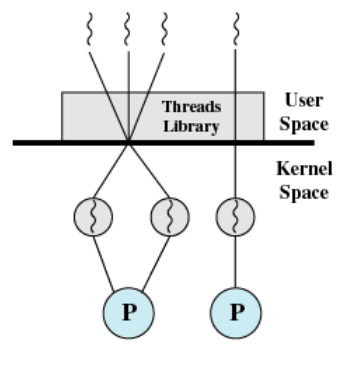
\includegraphics[width=0.50\textwidth]{approcci_misti}
	\end{figure}
	In questo approccio i thread vengono creati nello spazio utente e vari thread di uno stesso processo possono essere eseguiti contemporaneamente su più processori e una chiamata bloccante non blocca l'intero processo. \\
	Per fare questo, però, c'è necessità di comunicazione fra kernel e libreria di thread per mantenere un appropriato numero di kernel thread allocati nell'applicazioni. \\
	Il \textbf{Light Weight Process} o \textbf{LWP}, è una struttura intermedia che appare alla libreria dei thread utente come un processore virtuale sul quale schedulare l'esecuzione. \\
	Ad esempio, un'applicazione CPU-bound su un sistema monoprocessore implica che solo un thread alla volta può essere eseguiti quindi sarà sufficiente un unico LWP per thread. Su una applicazione I/O bound, invece, è richiesto un LWP per ciascuna chiamata di sistema bloccante.
	\subsection{Relazione tra thread e processi}
	\begin{tabular}{m{3,1cm} | m{5cm} | m{3cm}}
		\textbf{Thread:processi} &\textbf{Descrizione} & \textbf{Sistemi} \\
		\hline
		1:1 & Ogni thread di esecuzione è un processo unico con il proprio spazio di indirizzamento e le proprie risorse & Molte implementazioni di UNIX \\
		\hline
		M:1 & Ogni processo ha associato un proprio spazio di indirizzamento e delle risorse. In ogni processo si possono creare ed eseguire molti thread & Windows NT, Solaris, MACH, OS/2, OS/390 \\
		\hline
		1:M & Un thread può spostarsi da un processo all'altro, questo permette di spostare facilmente i thread tra sistemi diversi & Ra(Clouds), Emerald \\
		\hline
		M:M & Combina le proprietà degli approcci M:1 e 1:M & TRIX
	\end{tabular} \\ \quad \\
	Gli ultimi approcci vengono usati negli ambienti distribuiti dove i thread possono spostarsi tra più calcolatori.
	\section{Symmetric Multi Processing (SMP)}
	Un calcolatore con più processori presenta diverse caratteristiche:
	\begin{itemize}
		\item i processori condividono le stesse risorse;
		\item tutti i processori possono effettuare le stesse funzioni;
		\item ogni processore esegue una stessa copia del SO;
		\item ogni processore gestisce la schedulazione dei processi o thread disponibili.
	\end{itemize} 
	Non è facile, però, eseguire i compiti sopra elencati in quanto:
	\begin{itemize}
		\item i processori non devono schedulare lo stesso processo;
		\item ci deve essere comunicazione tra processori per quanto riguarda la memoria condivisa in quanto c'è la possibilità di effettuare accessi simultanei alla memoria;
		\item ci deve essere coerenza della cache che viene risolto a livello hardware.
	\end{itemize}
	Il sistema multiprocessore \textbf{deve essere trasparente all'utente} in quanto il programmatore deve operare cose se fosse in multiprogrammazione su monoprocessore. \\
	Nella progettazione di un Sistema Operativo per i sistemi multiprocessore ci sono diversi punti critici quali:
	\begin{itemize}
		\item processi e thread del kernel concorrenti, cioè l'esecuzione su diversi processori non deve compromettere le strutture di gestione del Sistema Operativo;
		\item la schedulazione, non devono esserci conflitti;
		\item la sincronizzazione: la mutua esclusione e l'ordinamento degli eventi;
		\item gestione della memoria condivisa;
		\item tolleranza ai guasti: in caso di perdita di un processore devono essere aggiornate le strutture di controllo del Sistema Operativo.
	\end{itemize}
	\section{Stati dei thread di Windows}
	Gli stati dei thread di Windows sono:
	\begin{itemize}
		\item \textbf{Ready};
		\item \textbf{Standby}: legato alla disponibilità del processore (SMP) richiesto per il thread. Se la priorità è sufficientemente alta il processo in running può essere interrotto;
		\item \textbf{Running};
		\item \textbf{Waiting}: in attesa di evento I/O, attesa per sincronizzazione;
		\item \textbf{Transition}: thread pronto per l'esecuzione ma le risorse non sono disponibili;
		\item \textbf{Terminated}
	\end{itemize}
	\begin{figure}[H]
		\centering
		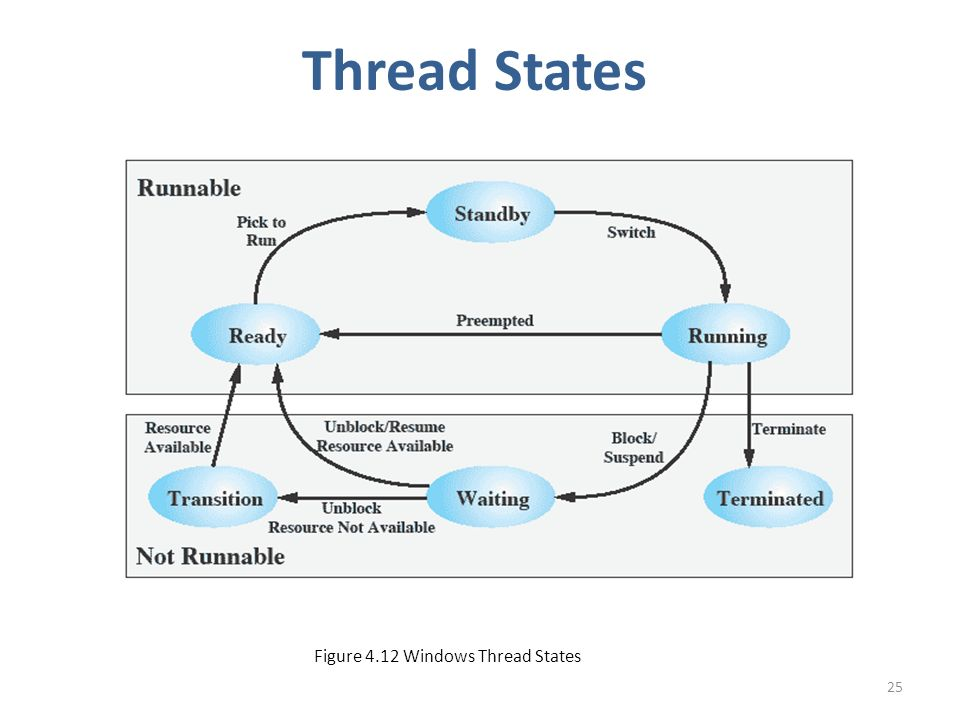
\includegraphics[width=1.00\textwidth]{windows_thread}
	\end{figure}
	C'è il supporto del SMP quindi tutte le tipologie di thread possono essere eseguiti su ogni processore; il primo thread in ready viene assegnato al primo processore disponibile; thread appartenenti allo stesso processo possono essere eseguiti contemporaneamente su diversi processori; esecuzione di un thread sempre sullo stesso processore cosi i dati sono ancora nella cache del processore.
	\section{MicroKernel}
	\begin{figure}[H]
		\centering
		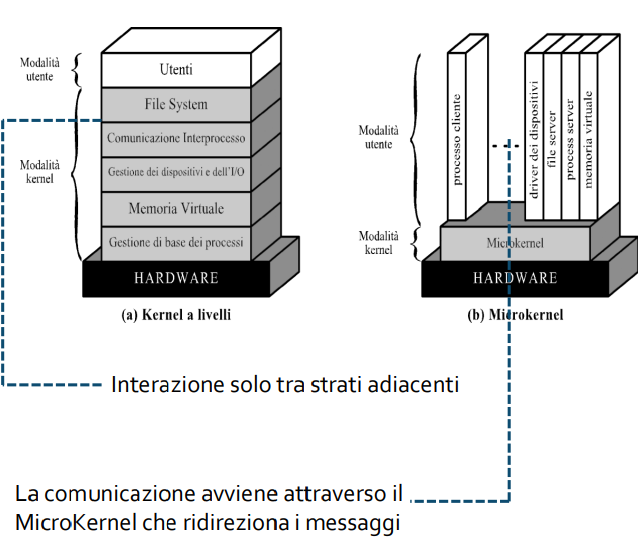
\includegraphics[width=1.00\textwidth]{microkernel}
	\end{figure}
	Il microkernel è un piccolo nucleo del sistema operativo che ne contiene solo le funzioni essenziali, mentre i servizi inclusi tradizionalmente nel Sistema operativo, come mostrato nella figura, sono sottosistemi esterni al microkernel ed eseguiti in modalità utente, come la gestione della memoria virtuale, i driver dei dispositivi, il file system ecc.
	\subsection{Vantaggi del microkernel}
	Il microkernel presenta diversi vantaggi quali:
	\begin{itemize}
		\item \textbf{interfaccia uniforme}: i moduli usano le stesse interfacce per le richieste al microkernel;
		\item \textbf{estensibilità}: introduzione di nuovi servizi o modifiche non richiedono modifiche del microkernel;
		\item \textbf{flessibilità}: a seconda delle applicazioni certe caratteristiche possono ridotte o potenziate per soddisfare al meglio le richieste dei clienti, come Windows home o professional o ultimate;
		\item \textbf{portabilità}: il cambio dell'hardware cambierà unicamente la modifica del microkernel;
		\item \textbf{affidabilità}: lo sviluppo di piccole porzioni di codici ne permette una migliore ottimizzazione e test;
		\item \textbf{supporto ai sistemi distribuiti}: ogni servizio è identificato da un numero nel microkernel e una richiesta da client non è necessario che sappia dove si trova il server in grado di soddisfare la stessa perchè la messaggistica è gestita dal microkernel.
	\end{itemize}
	\subsection{Design del microkernel}
	Il microkernel deve contenere:
	\begin{itemize}
		\item le funzioni che dipendono direttamente dall'hardware come la gestione degli interrupt e I/O;
		\item le funzioni per la comunicazione tra processi;
		\item gestione primitiva della memoria.
	\end{itemize}
	L'utilizzo del microkernel, però, porta diverse problematiche riguardanti le prestazioni del sistema perchè costruire, inviare, accettare e decodificare un messaggio costa più che fare una chiamata al SO e ci sono due possibili soluzioni a questo problema: la prima è quella di aggiungere funzionalità al microkernel, come fa il MACH OS in modo da ridurre il numero di cambiamenti di stato das utente a kernel però questo porta a interfacce minime alla riduzione di flessibilità ecc.; la seconda è un'ulteriore riduzione del microkernel.
	\subsection{Funzioni minime del microkernel}
	La prima funzione principale o minima del microkernel è la \textbf{gestione primitiva della memoria}. In questa funzione troviamo un modulo esterno al microkernel che mappa pagine virutali in pagine fisiche e il mapping viene conservato in memoria principale. 
	\begin{itemize}
		\item un'applicazione che accede ad una pagina che non si trova in memoria genera un page fault;
		\item l'esecuzione passa al microkernel che invia un messaggio al paginatore comunicando la pagina richiesta;
		\item la pagina viene caricata e in questa fase il paginatore e il kernel collaborano per il mapping della memoria reale in memoria virtuale;
		\item quando viene caricata la pagina il pager invia un messaggio all'applicazione.
	\end{itemize}\
	La seconda funzione del microkernel è la \textbf{comunicazione tra processi}. Un messaggio fra processi è formato dall'intestazione, dal corpo dal puntatore e le informazioni di controllo:
	\begin{itemize}
		\item \textbf{Intestazione}: mittente e ricevente;
		\item \textbf{Corpo}: dati del messaggio;
		\item \textbf{Puntatore}: informazioni di controllo del processo e blocco dati.
	\end{itemize}
	Ad ogni processo viene associata una \textbf{porta}: una capability list indica chi può inviare messaggi e questa porta viene amministrata dal kernel.\\
	La terza funzione del microkernel è la \textbf{gestione degli interrupt e I/O}. Il microkernel non gestisce direttamente gli interrupt ma li riconosce e \textbf{trasforma l'interrupt in messaggio a livello utente}, che invia al processo che gestisce gli interrupt.
	\begin{lstlisting}[style=pascalstyle]
		driver thread:
		do
			wait(msg, mittente);
			if (mittente=mio_intterupt_hardware)
				then leggi/scrivi le porte di I/O;
			azzera l'interrupt hardware
			else...
			Endif
		Enddo
	\end{lstlisting}
	\chapter{Gestione delle risorse e problematiche connesse}
	I processi utilizzano delle risorse che sono gestite e amministrate dal SO e il \textbf{sistema operativo decide in merito all'assegnazione delle risorse ai processi}, disponendo l'ordine di accesso dei processi a queste e le modalità di accesso. \\
	I processi utilizzano le risorse per tramite del Sistema Operativo, che trasmette le operazione agli strati sottostati per conto dei processi. \\
	La gestione delle risorse può portare a diverse problematiche che devono essere accuratamente attenzionate e queste problematiche sono legate alla concorrenza e alla mutua esclusione delle risorse. \\
	La\textbf{mutua esclusione} delle risorse significa che \textbf{una risorsa singola può essere assegnata a un solo processo alla volta}. 
	\section{Grafo di allocazione delle risorse}
	Un grafo di allocazione delle risorse rappresenta in che modo le risorse sono assegnate ai processi e le richieste dei processi:
	\begin{figure}[H]
		\centering
		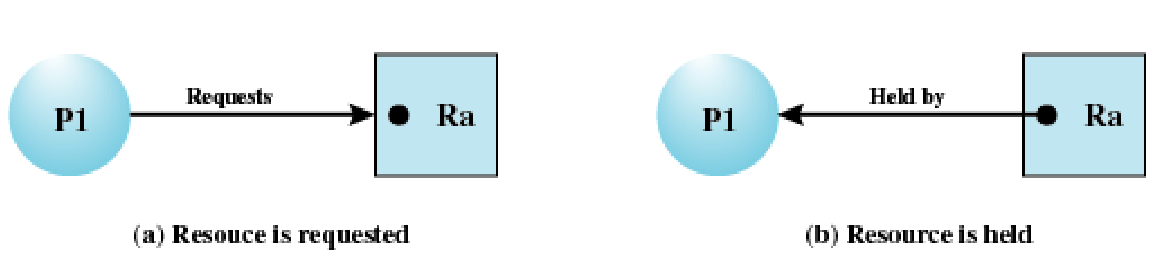
\includegraphics[width=0.8\textwidth]{allocazione_risorse}
	\end{figure}
	\section{Stallo dei processi}
	Lo \textbf{stallo dei processi} o \textbf{deadlock} è una delle condizioni problematiche che possono verificarsi nell'ambito della gestione delle risorse. \\
	La definizione di deadlock è: \textbf{un insieme di processi è detto in stallo se ciascun processo nell'insieme è in attesa di un evento che solo un altro processo dello stesso insieme può generare}. \\
	Lo stallo comporta che, essendo tutti i processi in attesa di un evento, sono nello stato di blocked, questa situazione comporta che nessuno dei processi in stallo può:
	\begin{itemize}
		\item passare in esecuzione perchè necessitano del verificarsi di un evento;
		\item rilasciare le risorse in quanto non può passare in esecuzione
	\end{itemize}
	I processi in stallo sono congelati in questa situazione a meno di un intervento da parte del SO o dell'amministratore.
	\subsection{Condizioni per lo stallo}
	Lo stallo dei processi per verificarsi necessita della congiunzione di quattro condizioni:
	\begin{enumerate}
		\item \textbf{mutua esclusione}, un solo processo alla volta può utilizzare una risorsa;
		\item \textbf{hold \& wait}, un processo può mantenere il possesso delle risorse allocate mentre attende di averne altre;
		\item \textbf{assenza di prerilascio}, i processi non possono essere forzati a rilasciare in anticipo le risorse acquisite;
		\item \textbf{\color{red}attesa circolare} un processo aspetta una risorsa che è occupata da un altro processo in attesa circolare
	\end{enumerate}
	Le prime tre condizioni sono delle condizioni derivanti direttamente dalla progettazione e sono necessarie ma non sufficienti, la quarta è la condizione che fa verificare la condizione di stallo e che rende sufficienti tutte le condizioni
	\subsection{Strategie per affrontare lo stallo}
	Sono possibili quattro diverse strategie per affrontare il problema dello stallo dei processi:
	\begin{enumerate}
		\item \textbf{ignorare il problema}, l'algoritmo dello struzzo;
		\item \textbf{consentire il verificarsi dello stallo, rilevarlo e risolverlo}
		\item \textbf{evitarlo con politiche di allocazione}: le tre condizioni necessarie sono permesse, un algoritmo verifica dinamicamente che una richiesta non produca una situazione di stallo;
		\item \textbf{impedirlo rimuovendone le condizioni}: progettare un SO in modo che la possibilità di avere uno stallo sia esclusa a priori tramite la negazione di una delle 4 condizioni.
	\end{enumerate}
	\section{Algoritmo dello struzzo}
	L'algoritmo dello struzzo pretende che il problema non esista ed è una soluzione ragionevole se: 
	\begin{itemize}
		\item lo stallo capita di rado;
		\item il costo per evitare lo stallo è troppo elevato.
	\end{itemize}
	Si ha quindi un compromesso tra convenienza e correttezza. \\
	Molte volte si utilizza questo approccio infatti Windows e UNIX utilizzano questo approccio.
	\section{Consentire lo stallo, rilevarlo e risolverlo}
	La seconda strategia possibile è quella di \textbf{consentire il verificarsi dello stallo, rilevarlo e risolverlo}. \\
	Questa strategia prevede di operare normalmente e verificare periodicamente se si è verificato uno stallo. \\
	Questa strategia può essere divisa in due fasi:
	\begin{enumerate}
		\item rilevare lo stallo;
		\item eliminare lo stallo.
	\end{enumerate}
	\subsection{Rilevare lo stallo}
	\begin{figure}[H]
		\centering
		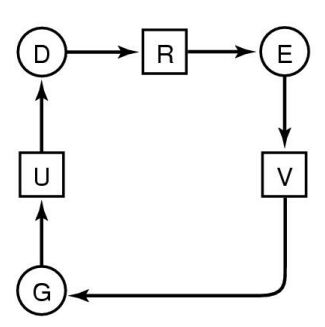
\includegraphics[width=1.00\textwidth]{deadlock}
	\end{figure}
	Avendo a disposizione una sola risorsa di ogni tipo, cioè una sola stampante, un solo mouse ecc, si può rilevare lo stallo costruendo il grafo di assegnazione delle risorse e un ciclo all'interno del grafo denota uno stallo. \\
	Questo è irragionevole da implementare in quanto molto complesso perchè le risorse disponibili sono molte ed è applicabile solo nei casi di una risorsa per tipologia. \\
	Perciò, serve una soluzione che funzioni in generale, cioè nei casi in cui si hanno più risorse per tipologia. \\
	Definiamo le strutture dati di cui necessitiamo:
	\begin{figure}[H]
		\centering
		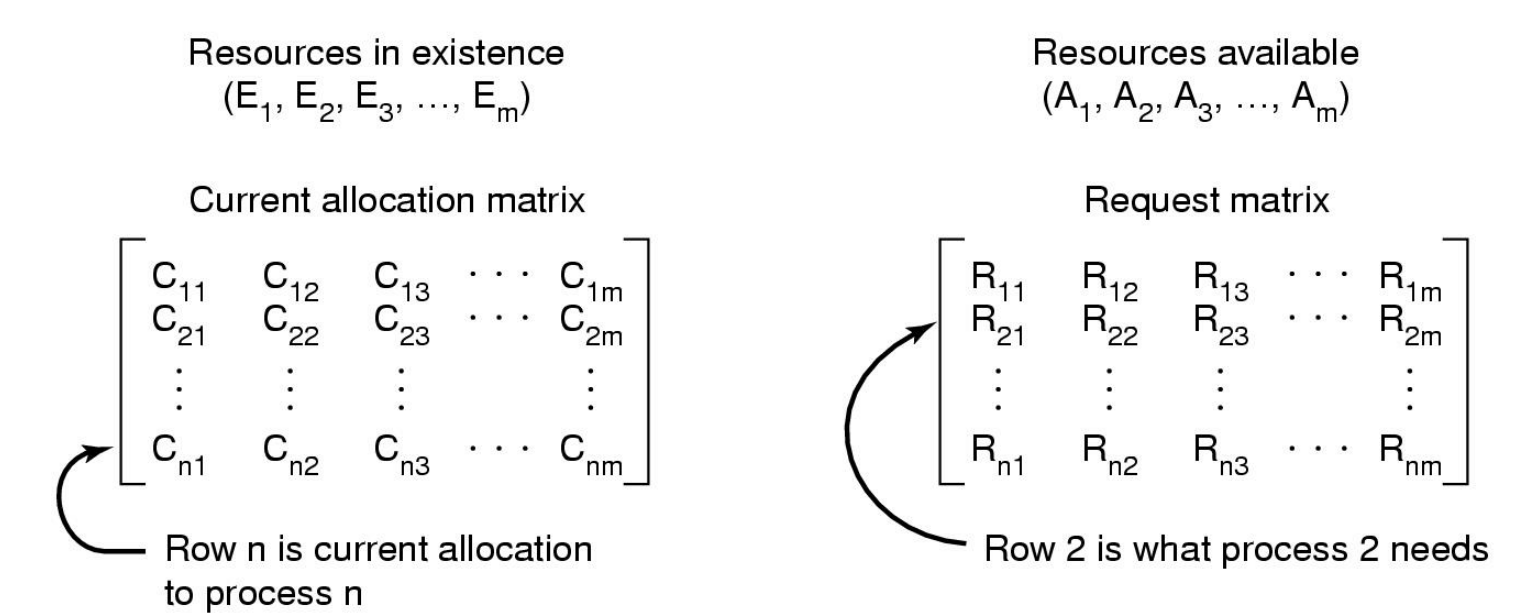
\includegraphics[width=1.00\textwidth]{rilevazione_stallo}
	\end{figure}
	Notazioni:
	\begin{itemize}
		\item Sia $R_i$ l'$i$-esima riga della matrice $R$
		\item Dati due vettori $X = [x_1, \dots, x_m]$ e $Y = [y_1, \dots, y_m]$ \\
		$X \leq Y \iff \forall\ i \in [1,m]\ x_i \leq y_i$
	\end{itemize}
	\begin{figure}[H]
		\centering
		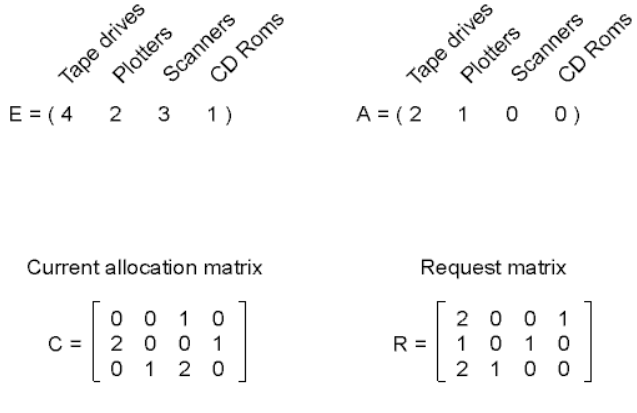
\includegraphics{rilevazione_stallo_generale}
	\end{figure}	
	L'\textbf{algoritmo di individuazione} dello stallo funziona nel seguente modo:
	\begin{enumerate}
		\item inizialmente ogni processo $P_i$ non è marcato
		\item Per ogni processi non marcato $P_i$ tale che $R_i \leq A$, cioè individuo i processi che possono ottenere le risorse necessarie alla sua terminazione
		\begin{itemize}
			\item $A = A + C_i$
			\item marca $P_i$
		Qui il processo può terminare la sua normale esecuzione e ne rilascia le risorse
		\end{itemize}
		\item Se rimangono processi non marcati i processi non marcati sono in stallo, cioè nessuno di loro può acquisire risorse sufficienti a terminare, tenendo occupate le risorse già prese.
	\end{enumerate}
	Quando e quanto spesso invocare l'algoritmo dipende da:
	\begin{itemize}
		\item frequenza presunta con la quale si verifica lo stallo;
		\item numero di processi coinvolti nello stallo.
	\end{itemize}
	Uno stallo si verifica quando un processo avanza una richiesta che non può essere soddisfatta immediatamente. \\
	\textbf{Utilizzo dell'algoritmo a ogni richiesta}: consente la determinazione dello stallo e del processo la cui richiesta ha dato origine allo stallo, però questo appesantisce di molto il sistema. \\
	\textbf{Utilizzare l'algoritmo quando la percentuale di utilizzo delle risorse scende al di sotto di una soglia} \\
	\textbf{Utilizzare l'algoritmo ad instanti arbitrari}: nel grafo di assegnazione delle risorse potrebbero esistere molti cicli e diventa difficile determinare quale processo ha causato lo stallo.
	\subsection{Eliminare lo stallo}
	Si può operare secondo diverse modalità:
	\begin{itemize}
		\item tramite \textbf{terminazione dei processi}:
		\begin{itemize}
			\item abort di tutti i processi coinvolti nello stallo. Soluzione comunemente adottata. 
			\item abort di un processo alla volta fino a quando il ciclo non è eliminato. Dopo ogni abort si deve rieseguire l'algoritmo di determinazione dello stallo. L'ordina con cui abortire i processi è dato dalla funzione di minimo costo basata su:
			\begin{itemize}
				\item priorità dei processi;
				\item tempo trascorso in esecuzione e necessario al completamento;
				\item risorse già utilizzate e risorse richieste;
				\item tipo di processo.
			\end{itemize}			
		\end{itemize}
		\item tramite \textbf{prelazione di risorse}
		\begin{itemize}
			\item selezionare un processo vittima tramite la funzione di minimo costo;
			\item rollback del processo a cui è stata sottratta la risorsa - return ad uno stato sicuro per poterlo riavviare in seguito. \\
			Salvataggio periodico dello stato dei processi. In caso di stallo:
			\begin{itemize}
				\item si ripristina il processo all'ultimo stato salvato;
				\item si fa ripartire il processo, il non-determinismo dei processi dovrebbe garantire il non ri-verificarsi dello stallo.
			\end{itemize}
			In generale conviene uccidere il processo
			\item starvation, alcuni processi potrebbero essere selezionati costantemente come vittime e quindi bisogna includere come fattore il numero di rollback.
		\end{itemize}
	\end{itemize}
	\section{Evitare lo stallo con politiche di allocazione}
	\begin{figure}[H]
		\centering
		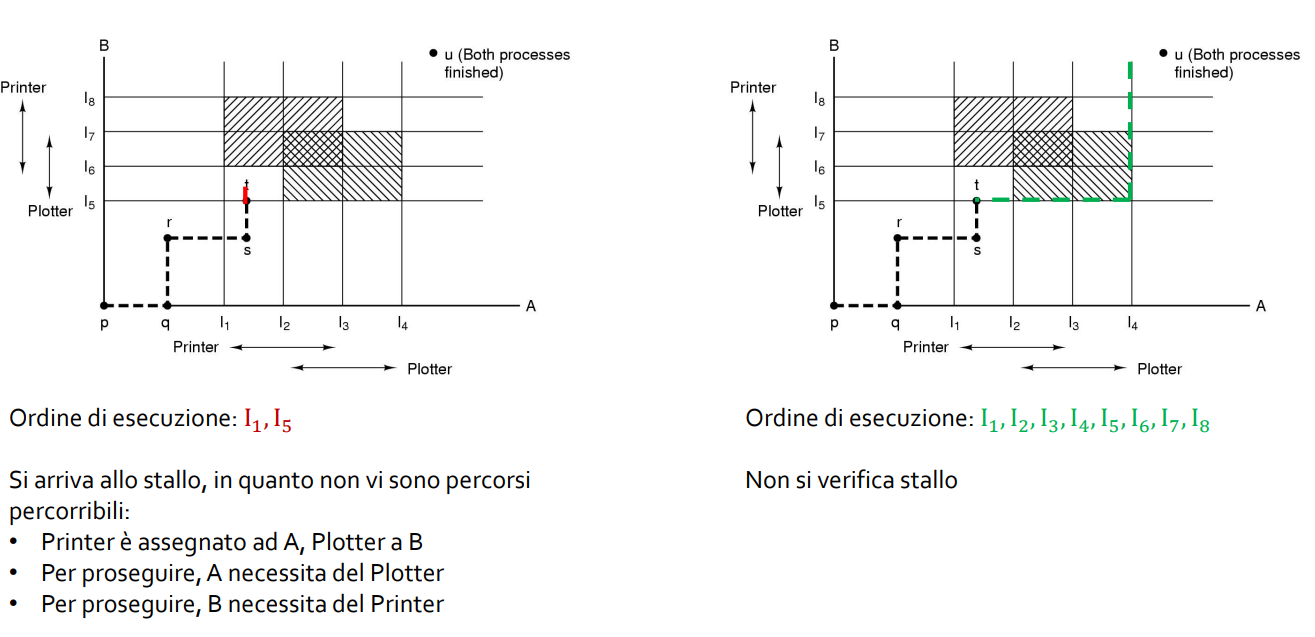
\includegraphics[width=1.00\textwidth]{evitare_stallo}
	\end{figure}
	Questa strategia presenta alcuni vantaggi e svantaggi:
	\begin{itemize}
		\item \textbf{Vantaggi}: non è necessario interrompere i processi e riportarli in uno stato precedente
		\item \textbf{Svantaggi}:
		\begin{itemize}
			\item il numero massimo di risorse necessitate da ogni processo deve essere noto a priori;
			\item i processi devono essere indipendenti: l'ordine di esecuzione non deve essere vincolato da esigenze di sincronizzazione;
			\item deve esserci un numero fissato di risorse da allocare;
			\item quando un processo richiedere risorse potrebbe essere posto in attesa;
			\item quando un processo ottiene tutte le risorse di cui necessita, deve rilasciarle in un tempo finito.
		\end{itemize}
	\end{itemize}
	\subsection{Stato sicuro e insicuro}
	Si possono definire due stati del sistema rispetto alle risorse assegnate:
	\begin{enumerate}
		\item \textbf{stato sicuro}: esiste almeno una sequenza di esecuzione dei processi che ne consente la terminazione senza incorrere in una situazione di stallo
		\item \textbf{non sicuro}
	\end{enumerate}
	Lo stato sicuro garantisce l'impossibilità di verificarsi dello stallo, mentre, lo stato non sicuro indica che c'è la possibilità ma non la certezza che si verifichi uno stallo. \\
	\textbf{Deadlock avoidance} significa quindi assicurarsi che il sistema non entri mai in uno stato non sicuro. \\
	Segue un'esempio di stato sicuro e insicuro:
	\begin{figure}[H]
		\centering
		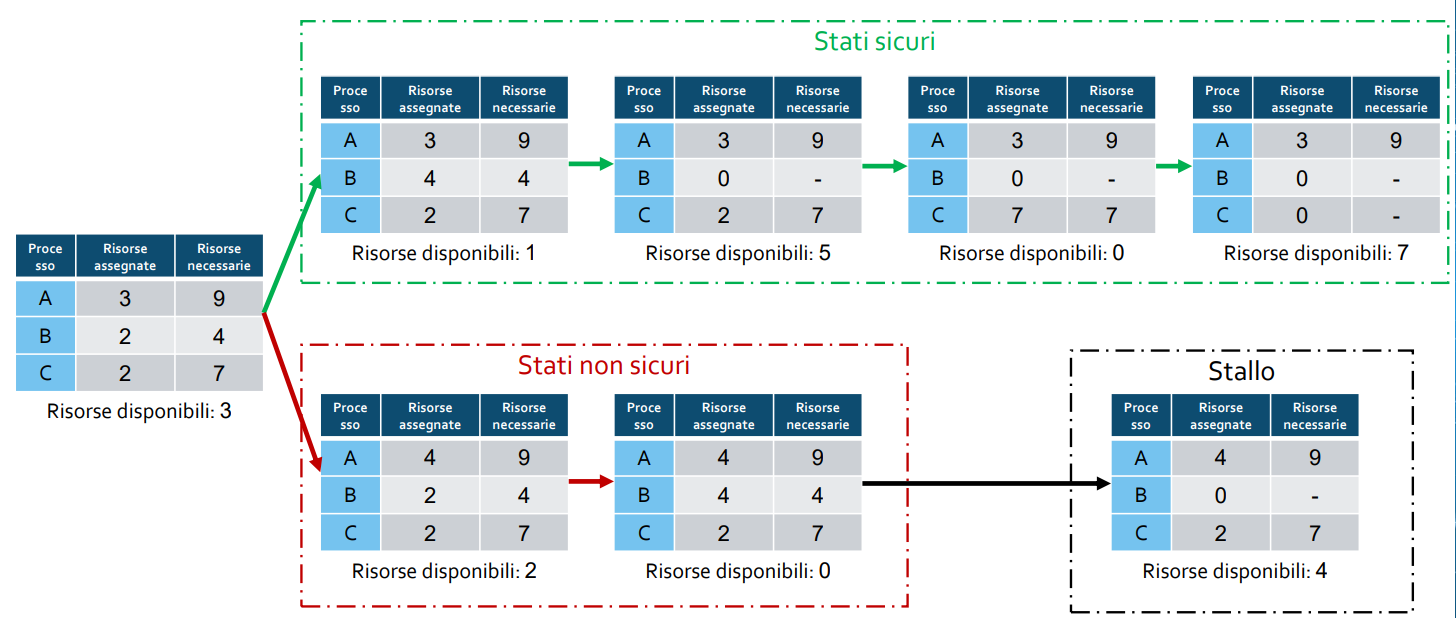
\includegraphics[width=1.00\textwidth]{stato_sicuro_nonsicuro}
	\end{figure}
	\subsection{Algoritmo del banchiere}
	La strategia di evitare lo stallo secondo politiche di allocazione vede la sua applicazione con l'uso dell'\textbf{algoritmo del banchiere}. \\
	Questo algoritmo assegna risorse al processo solo se il sistema resta in uno stato sicuro, cioè i processi procedono, terminano e restituiscono le risorse al sistema e lo stato sicuro viene determinato mediante l'uso dell'algoritmo di rilevazione dello stallo. \\
	Codice dell'algoritmo: \\
	\begin{lstlisting}[style=pascalstyle]
		//global data structures
		struct state
		{
			int resource[m];
			int available[m];
			int claim[n][m];
			int alloc[n][m];
		}
		
		//resource alloc algorithm
		if (alloc [i, *] + request [*] > claim [i, *])
			< error >;
		else if (request [*] > available [*])
			< suspend process > ;
		else 
		{
			< define newstate by: 
			alloc [i, *] = alloc [i, *] + request [*];
			available [*] = available [*] - request [*] >
		}
		if (safe (newstate))
			< carry out allocation >;
		else 
		{
			< restore original state >;
			< suspend process >;
		}
		
		//test for safety algorithm (banker's algorithm)
		boolean safe (state S)
		{
			int currentavail[m];
			process rest[< number of processes >];
			currentavail = available;
			rest = (all processes);
			possible = true;
			while (possible) 
			{
				< find a process $P_k$ in rest such that 
					claim [k, *] - alloc [k, *] <= currentavail;>
				if (found)
				{
					currentavail = currentavail + alloc[k, *];
					rest = rest - {$P_k$};
				} 
				else
					possible = false;
			}
			
				return (rest == null);
		}
	\end{lstlisting}
	\section{Impedire lo stallo rimuovendone le condizioni}
	Questa strategia impedisce il verificarsi dello stallo rimuovendo una delle quattro condizioni e quindi, si impongono dei vincoli sulla richiesta delle risorse. \\
	Le classi di prevenzione sono:
	\begin{itemize}
		\item \textbf{metodi indiretti}: prevengono il verificarsi di una delle tre condizioni necessarie;
		\item \textbf{metodi diretti}: prevengono il verificarsi dell'attesa circolare
	\end{itemize}
	\subsection{Negare la mutua esclusione}
	\begin{itemize}
		\item un processo non deve mai attendere una risorsa condivisibile;
		\item devono essere possibili accessi multipli contemporanei alle risorse condivise;
	\end{itemize}
	Questo algoritmo potrebbe funzionare in alcuni casi, ma in altri casi, ad esempio quando la risorsa in questione è il mouse, non possono esserci accessi multipli e quindi l'algoritmo non è applicabile in generale. \\
	Come dicevo, in alcuni casi specifici, ad esempio nel caso in cui la risorsa in questione è una stampante, che è un dispositivo gestibile con spool, l'algoritmo è utilizzabile:
	\begin{itemize}
		\item i processi scrivono l'output in un'area di spool;
		\item solo il gestore della stampante richiede e usa la stampante;
	\end{itemize}
	Non tutti i dispositivi però possono essere gestiti con spool, inoltre, si può verificare lo stallo sullo spool. \\
	Il principio è quello di non assegnare una risorsa se non strettamente necessario e fare in modo che il minor numero di processi possa richiedere una risorsa.
	\subsection{Negare l'hold \& wait}
	Con questa strategia ogni processo dovrebbe richiedere all'inizio dell'esecuzione tutte le risorse. Questo però comporta dei problemi perchè il processo potrebbe non sapere di quali risorse avrà bisogno, il processo entra in blocked fino a quando tutte le richieste non vengono soddisfatte contemporaneamente e potrebbe bloccare delle risorse che altri processi potrebbero utilizzare. \\
	Questo quindi è un approccio inefficiente perchè prima di andare in run tutte le risorse dovrebbero essere disponibili quando in realtà potrebbe procedere solo con una parte di esse e le risorse che vengono assegnate a un processo potrebbero rimanere inutilizzate per molto tempo e quindi gli altri processi rimangono in attesa per un tempo non definito.
	\subsection{Negare l'assenza di prerilascio}
	Questo approccio può essere applicato in 2 modi:
	\begin{enumerate}
		\item un processo che non riesce ad ottenere le risorse di cui necessita, rilascia quelle che detiene per richiederle nuovamente in un istante successivo;
		\item il Sistema Operativo può richiedere il pre-rilascio delle risorse al processo che le detiene per assegnarle al richiedente
	\end{enumerate}
	Questo approccio è applicabile se lo stato della risorsa si può salvare facilmente, come nel caso della CPU, ma non applicabile nel caso delle stampanti ad esempio. \\
	Infatti, ipotizziamo un caso reale di utilizzo della stampante: supponiamo che una stampante stia stampando dopo una richiesta da parte del processo e successivamente questo processo viene forzato a rilasciare le risorse per assegnarle a un altro processo e la stampante smette di stampare quello che stava stampando precedentemente per iniziare a stampare ciò che richieder il nuovo processo e questo è assurdo.
	\subsection{Negare l'assenza circolare}
	In questo approccio si definisce un ordine lineare di numerazione per tutte le risorse, quindi se un processo richiedere una risorsa $R$, successivamente potrà richiedere solo una risorsa che nell'ordinamento segue $R$. \\
	Ad esempio, se $R_i$ precedere $R_j$ il processo potrà richiedere le risorse nell'ordine $R_i, R_j$. \\
	Questo metodo però può essere inefficiente.
	\section{Concorrenza}
	Dobbiamo definire alcuni concetti:
	\begin{itemize}
		\item \textbf{multiprogrammazione}: gestione di più processi su un singolo processore;
		\item \textbf{multiprocessing}: gestione di più processi su più processori;
		\item \textbf{processi distributi}: cluster.
	\end{itemize}
	La concorrenza è la \textbf{competizione tra processi (threads) per ottenere e condividere le risorse}
	\subsection{Terminologia della concorrenza}
	\begin{itemize}
		\item \textbf{sessione critica:} porzione di codice all'interno di un processo (thread) che richiede accesso a risorse condivise;
		\item \textbf{deadlock}: situazione nella quale due o più processi sono impossibilitati dal procedere perchè sono in attesa l'uno dell'altro;
		\item \textbf{livelock}: situazione nella quale due o più processi cambiano continuamente il proprio stato a causa del cambiamento di stato degli altri senza fare del lavoro utile;
		\item \textbf{mutua esclusione}: requisito per il quale, quando un processo è nella propria sezione critica, nessun altro processo può essere nella propria sezione critica se questa fa riferimento a risorse condivise con il primo processo;
		\item \textbf{race condition}: situazione nella quale thread o processi leggono e scrivono un dato condiviso e il risultato dipende dalla loro velocità reciproca;
		\item \textbf{starvation}: situazione nella quale un processo non riceve mai l'utilizzo di una risorsa e viene costantemente scavalcato da altri processi.
	\end{itemize}
	\subsection{Vantaggi e problemi della concorrenza}
	I vantaggi della concorrenza riguardano un migliore utilizzo delle risorse e i benefici che ne si ricavano sull'esecuzione nonostante il sovraccarico a causa del context switching. \\
	I problemi della concorrenza, nel caso di singolo processore, possono essere: 
	\begin{itemize}
		\item una \textbf{condivisione pericolosa}: ordine delle operazioni di lettura e scrittura su aree di memoria condivise;
		\item difficoltà nell'assegnare le risorse ai processi in maniera ottimale;
		\item difficoltà nella rilevazione degli errori nel codice e dei conflitti di interlacciamento, cioè l'esecuzione dei processi paralleli. 
	\end{itemize}
	Consideriamo un esempio della procedura \textit{echo}:
	\begin{lstlisting}[style=pascalstyle]
		char in, out;
		void echo() 
		{
			scanf("%c", &in);
			out = in;
			printf("%c", out);
		}
	\end{lstlisting}
	Supponiamo che si siano due processi concorrenti, $P_1$ e $P_2$:
	\begin{figure}[H]
		\centering
		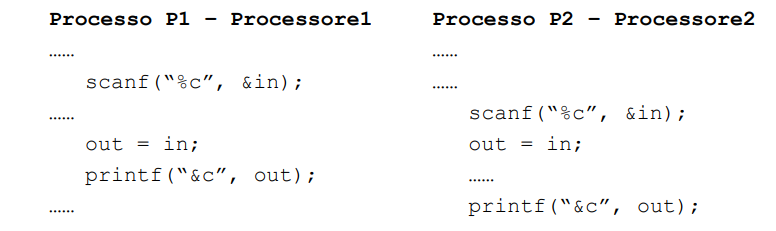
\includegraphics[width=1.00\textwidth]{interlacciamento}
	\end{figure}
	In questo caso il carattere letto da $P_1$ viene perso perchè $P_1$ esegue la scanf, viene interrotto, $P_2$ viene eseguito per intero e $P_1$ riprende l'esecuzione ma ora il carattere letto da $P_1$ viene sovrascritto da $P_2$. \\
	La soluzione di questo problema è la \textbf{mutua esclusione}, cioè l'esecuzione seriale dei programmi.
	\subsection{Mutua esclusione}
	I meccanismo che provvedono alla mutua esclusione devono garantire a:
	\begin{itemize}
		\item un solo processo alla volta deve accedere alla sezione critica;
		\item un processo fuori dalla sezione critica non deve interferire con il processo nella sezione critica;
		\item ogni processo deve poter accedere dopo un tempo finito di attesa in coda alla sezione critica, quindi non c'è starvation o stallo;
		\item se nessun processo è nella sezione critica, un processo deve avere la possibilità di entrarci senza attese;
		\item non ci devono essere supposizioni sulla velocità di esecuzione relative dei processi;
		\item il tempo di permanenza nella sezione critica è definito.
	\end{itemize}
	I meccanismi che provvedono alla mutua esclusione sono: 
	\begin{itemize}
		\item \textbf{Approcci software}: i processi, senza aiuto del SO o del linguaggio di programmazione, devono coordinarsi tra loro tramite l'\textbf{algoritmo Dekker}
		\begin{itemize}
			\item aumento del tempo di esecuzione;
			\item errori frequenti
		\end{itemize}
		\item utilizzo di particolari \textbf{istruzioni macchina} come \textit{test-set, scambio}:
		\begin{itemize}
			\item riduzione del sovraccarico;
			\item non soddisfacenti.
		\end{itemize}
		\item \textbf{Supporto del sistema operativo o del linguaggio di programmazione}:
		\begin{itemize}
			\item scambio messaggi (Inter-Process Communication);
			\item semafori;
			\item monitor.
		\end{itemize}
	\end{itemize}
	\subsection{Algoritmo di Dekker}
	\paragraph{Tentativo n.1}
	Nel primo tentativo dell'algoritmo di Dekker si applica, quello che viene chiamato \textbf{protocollo dell'Igloo}, che fa riferimento ai rifugi a forma di cupola costruiti con blocchi di neve la cui porta permette l'entrata di una sola persona alla volta. Applicando questo concetto ai processi, essi, prima di entrare nella sezione critica, controllano uno alla volta una variabile \textit{turno}. \\
	Algoritmo: \\
	\begin{lstlisting}[style=pascalstyle]
		var turno = 0..1; //variabile globale condivisa con due valori, 0 e 1
		Processo 0:						
		while (turno != 0)									
				{nulla} //busy wait			
		<sezione critica>;				
		turno = 1;						
		
		Processo 1:
		while (turno != 1)
				{nulla} //busy wait
		<sezione critica>;
		turno = 0;	
	\end{lstlisting}
	Notiamo, quindi, che se un processo deve aspettare il suo turno entra in un ciclo dove non succede nulla e quindi viene generata la \textbf{busy wait}, cioè l'\textbf{attesa attiva} che toglie tempo utile all'esecuzione. Il pro di questo tentativo è che garantisce la mutua esclusione in quanto un processo per poter iniziare la sua esecuzione deve attendere il suo turno, d'altra parte, però, se un processo è lento questo determina la velocità di avanzamento di entrambi i processi e se un processo fallisce nella propria sezione critica e non, questo non arriverà mai all'istruzione per cambiare il turno e quindi anche l'altro rimane bloccato per sempre. \\
	\paragraph{Tentativo n.2} In questo tentativo, ogni processo ha un flag relativo all'utilizzo della risorsa e può leggere il flag dell'altro senza modificarlo. \\
	Algoritmo:
	\begin{lstlisting}[style=pascalstyle]
		boolean flag[2];
		Processo 0:
		//mentre il processo 1 sta utilizzando la risorsa
		//il processo 0 non fa nulla e aspetta
		while(flag[1]) 
			{nulla};
		flag[0] = true; //indica che il processo 0 sta utilizzando la risorsa
		<sezione critica>;
		flag[0] = false; //indica che il processo 0 non sta utilizzando la risorsa
	\end{lstlisting}
	L'aspetto positivo di questo approccio è che se un processo fallisce fuori dalla sua sezione critica, l'altro può continuare a lavorare, d'altra parte se un processo fallisce entro la sezione critica o prima che questo abbia settato il suo flag a false allora l'altro rimane bloccato per sempre. Inoltre, se entrambi i processi vedono il flag dell'altro a false, mettono il loro flag a true ed entrano entrambi contemporaneamente nella sezione critica andando a violare la mutua esclusione.
	\paragraph{Tentativo n.3} 
	In questo tentativo, viene riutilizzata la stessa tecnica del tentativo precedente con la sola differenza che i processi, prima ancora di controllare se l'altro processo è nella sezione critica, dichiarano la propria volontà di entrare in sezione critica settando la flag a true, però in questo modo, se entrambi i processi settano la propria flag a true prima ancora che uno dei due verifichi la condizione del while entrambi andranno in busy wait e si genera uno stallo. 
	Algoritmo:
	\begin{lstlisting}[style=pascalstyle]
		boolean flag[2];
		
		Processo 0:
		//prima del test esprimo la volonta' di entrare in sezione critica
		flag[0] = true 
		while(flag[1])
			{nulla};
		<sezione critica>;
		flag[0] = false;
	\end{lstlisting}
	L'aspetto positivo di questo approccio è che non viola la mutua esclusione, ma oltre al problema del deadlock precedentemente descritto si genera sempre il solito problema che se un processo fallisce nella propria sezione critica l'altro rimane bloccato per sempre.
	\paragraph{Tentativo n.4} In questo approccio viene usata la tecnica precedente ma viene evitata la situazione di deadlock, generando però una situazione di attesa attiva. 
	\begin{lstlisting}[style=pascalstyle]
		Processo 0:
		flag[0] = true
		while (flag[1]) 
		{
			flag[0] = false;
			<pausa>;
			flag[0] = true; 
		}
		<sezione critica>;
		flag[0] = false;
		
		Processo 1:
		flag[1] = true 
		while (flag[0]) 
		{
			flag[1] = false;
			<pausa>;
			flag[1] = true; 
		}
		<sezione critica>;
		flag[1] = false;
	\end{lstlisting}
	Quello che succede in questo algoritmo è che i due processi settano la propria flag a true ed entrano nel ciclo, dopodichè settano la flag a false e c'è un ciclo di attesa, dopo di esso, settano nuovamente la flag a true, essenzialmente i due processi fanno questo: P0: "Vado io", P1: "Vado io", P0: "Non vado io", P1: "Non vado io" e questo genera un attesa attiva. Non è uno stallo in quanto il processo che riesce ad uscire prima dal ciclo di attesa riesce ad entrare nella sezione critica. Il solito problema che si presenta è che se un processo fallisce nella propria sezione critica l'altro rimane bloccato per sempre, d'altro canto però questo approccio garantisce la mutua esclusione.
	\paragraph{Soluzione corretta}
	Ogni processo ha una propria variabile \textbf{flag} che indica la volontà di entrare nella sezione critica. Inoltre, c'è una variabile \textbf{turno} che specifica chi ha il diritto di insistere nel tentativo di entrare nella propria sezione critica. \\
	Ad esempio, se il processo 0 vuole entrare nella sezione critica pone il suo flag a true, dopodichè controlla la flag del processo 1, se questa è falsa entra nella sezione critica, se questa è vera controlla il turno, se il turno è 0 (il suo) controlla periodicamente la flag del processo 1, se il turno è 1 quindi del processo 1 pone la sua flag a false lasciando passare il processo 1. \\
	Algoritmo:
	\begin{lstlisting}[style=pascalstyle]
		boolean flag[2];
		int turno;
		void main() {
			flag[0] = false;
			flag[1] = false;
			turno = 1;
			processo P0;
			processo P1;
		}
		
		Processo P0:
		{
			flag[0] = true
			while (flag[1]) {
				if (turno == 1) {
					flag[0] = false;
					while (turno == 1) 
						{nulla}; //Attesa attiva
					flag[0] = true;
				}
			}
			<sezione critica>;
			flag[0] = false;
		}
	\end{lstlisting}
	L'algoritmo di dekker è un algoritmo complesso e nei casi analizzati abbiamo trattato solo i casi di due processi, ma se dovessimo immaginarlo per un numero di processi maggiore questo algoritmo diventa veramente complesso. Inoltre, rimane sempre il problema dell'attesa attiva quando un processo controlla il flag dell'altro processo se pari a true e rimane sempre il problema che se un processo fallisce nella propria sezione critica l'altro rimane bloccato per sempre.
	\subsection{Supporti hardware}
	Nelle macchine monoprocessore i processi si alternano in esecuzione. Per garantire la mutua esclusione è possibile evitare l'interruzione di un processo attivando e disattivando gli interrupt, quindi tramite supporto hardware. Praticamente quello che accade è questo:
	\begin{center}
		\textit{$\langle$disattiva le interruzion$\rangle$} \\
		\textit{$\langle$sezione critica$\rangle$} \\
		\textit{$\langle$attiva le interruzioni$\rangle$}
	\end{center}
	Così facendo la mutua esclusione viene garantita, però l'efficienza del sistema peggiora in quanto il processore non può alternare i processi liberamente e non funziona su macchine SMP, cioè una macchina a più processori. \\
	La soluzione per le macchine SMP (Symmetric Multi Processing) è di avere istruzioni macchina speciali per l'accesso a locazioni di memoria in modo atomico, cioè non interrompibile e l'accesso sequenziale ad una locazione di memoria è garantito dall'hardware. Quindi, a differenza dell'algoritmo di Dekker che era un approccio software, indipendente dal sistema operativo e dall'hardware, questa tipologia di soluzione dipende invece dall'hardware. \\
	Le istruzioni macchina speciali che permettono l'accesso serializzato alle locazioni di memoria sono:
	\begin{itemize}
		\item test-and-set;
		\item scambio(swap).
	\end{itemize}
	Se si eseguono due test-and-set contemporaneamente queste vengono serializzate.
	\paragraph{\color{red}Test \& set}: \\
	\begin{lstlisting}[style=pascalstyle]
		boolean test_and_set(boolean *target) {
			boolean val = *target;
			*target = TRUE;
			return val;
		}
	\end{lstlisting}
	Vediamo un utilizzo di questa funzione per garantire mutua esclusione. \\
	Sia \textit{lock} una variabile condivisa inizializzata a false per indicare che la risorsa è libera.
	\begin{lstlisting}[style=pascalstyle]
		boolean lock = false;
		while (true) {
			while (test_and_set(&lock))
				; //non fare niente
			<sezione critica>;
			lock = FALSE; //rilascio della risorsa
		}
	\end{lstlisting}
	La funzione \textit{test\_and\_set} si salva il valore iniziale della risorsa, cioè se è accessibile o meno, lo setta a true, ma restituisce il valore iniziale. In questo modo se il processo 0 vuole utilizzare la risorsa, la funzione restituisce false e non entra nel ciclo e setta la variabile lock a true ed entra nella propria sezione critica, di conseguenza se un altro processo tenta di accedere alla risorsa, la variabile lock ora vale true perchè il processo 0 è ancora nella sezione critica, quindi la funzione restituisce true e il processo 1 entra in un ciclo di attesa fino a quando il processo 0 non esce dalla sezione critica e rilascia la risorsa.
	\paragraph{\color{red}Swap}: \\
	\begin{lstlisting}[style=pascalstyle]
		void swap(boolean *a, boolean *b) {
			boolean temp = *a;
			*a = *b;
			*b = temp;
		}
	\end{lstlisting}
	Vediamo un utilizzo della funzione swap per garantire la mutua esclusione. \\
	Sia \textit{lock} una variabile condivisa settata a false per indicare che la risorsa è accessibile e \textit{key} la volontà di entrare nella sezione critica.
	\begin{lstlisting}[style=pascalstyle]
		while (true) {
			key = true;
			while (key == true)
				swap (&lock, &key); //lock diventa true e key diventa false
			<sezione critica>;
			lock = false;
		}
	\end{lstlisting}
	La mutua esclusione è garantita dalla stessa situazione spiegata precedentemente con la sola differenza che quando lock è true, key rimane true e quindi il secondo processo rimane in attesa fino a quando il primo processo non rilascia la risorsa.
	\paragraph{Vantaggi e svantaggi dei supporti hardware}
	La tecnica dei supporti hardware si può applicare a un qualsiasi numero di processi anche su multiprocessori a memoria condivisa e si possono usare per gestire anche più di una sezione critica ciascuna con una propria variabile. Il problema, però, è che c'è sempre un'attesa attiva e quindi i processi consumano tempo di CPU, ci può essere starvation perchè se gli algortimi di scheduling che sono stati scelti causano starvation, di conseguenza anche lo scheduler soffrirà di starvation, infatti la scelta di quale processo dovrà andare nella sezione critica è arbitraria. Inoltre, i supporti hardware possono causare stallo, ad esempio, se il processore è singolo, il processo P1 è in sezione critica, P2 ha priorità più alta di P1 e tenta di accedere tramite test and set o swap alla risorsa che è bloccata da P1 e nella sua attesa attiva non lascierà mai il posto a P1 in quanto ha priorità più bassa e quindi si genera uno stallo.
	\subsection{Supporto del Sistema operativo e dei linguaggi di programmazione}
	Le soluzioni offerte dal Sistema operativo e dai linguaggi di programmazioni sono i \textbf{semafori} e i \textbf{monitor}. \\
	Il semaforo può essere binario, cioè gestisce una sola risorsa o contatore, cioè gestisce un lotto di risorse dello stesso tipo. \\
	Il \textbf{semaforo} è una variabile booleana o intera sulla quale sono possibili 3 operazioni:
	\begin{enumerate}
		\item inizializzazione ad un valore non negativo, nel caso del booleano viene settato a true, nel caso sia intera viene settata al numero di risorse da gestire, ad esempio se sono 5 stampanti, viene settato a 5;
		\item operazione atomica \textbf{wait()}: decrementa il valore della variabile. Se il valore della variabile diventa negativo, il processo che ha eseguito la wait viene bloccato;
		\item operazione atomica \textbf{signal()}: incrementa il valore della variabile. Se il valore della variabile era negativo, uno dei processi bloccati nell'operazione di wait viene sbloccato.
	\end{enumerate}
	\textbf{Funzionamento del semaforo}:
	\begin{enumerate}
		\item si associa un semaforo ad ogni risorsa condivisa;
		\item il processo che vuole utilizzare la risorsa effettua un'operazione di wait;
		\item il processo che rilascia la risorsa effettua il signal;
		\item la variabile numerica indica il numero di istanze di una risorsa condivisa;
		\item se la variabile è negativa, il valore assoluto di essa rappresenta il numero di processi in attesa
	\end{enumerate}
	\paragraph{Implementazione del semaforo contatore}:
	\begin{lstlisting}[style=pascalstyle]
		typedef struct {
			int istanze;
			struct processo	*P; //lista dei processi in coda
		} semaforo;
		
		void wait(semaforo s) {
			s.istanze--;
			if (s.istanze < 0) {
				<poni processo in coda>
				<blocca questo processo: running->blocked >
			}
		}
		
		void signal(semaforo s) {
			s.instanze++;
			if (s.istanze <= 0) {
				<rimuovi processo in coda>
				<sveglia il processo: blocked->ready >
			}
		}
	\end{lstlisting}
	\paragraph{Implementazione del semaforo binario}:
	\begin{lstlisting}[style=pascalstyle]
		typedef struct {
			boolean val;
			struct processo	*P; //lista dei processi in coda
		} semaforo_bin;
		
		void wait(semaforo s) {
			if (s.val == true) {
				s.val == false;
			} else {
				<poni processo in coda a P>
				<blocca questo processo: running->blocked >
			}
			
		}
		
		void signal(semaforo s) {
			if (*P == NULL) { //coda vuota
				s.val = true;
			} else {
				<rimuovi un processo dalla coda>
				<sveglia il processo: blocked->ready >
			}
		}
	\end{lstlisting}
	\paragraph{Atomicità di wait e signal} Come possiamo fare affinchè wait e signal siano atomiche? \\
	\begin{enumerate}
		\item \textbf{implementarle in hardware o firmware};
		\item Utilizzare l'algoritmo di Dekker o Peterson ma ci sarebbe un sovraccarico di elaborazione;
		\item \textbf{Utilizzo dell'istruzione atomica test\&set}
		\item Se il sistema è monoprocessore basta disattivare gli interrupt durante le operazioni
	\end{enumerate}
	I semafori non presentano attesa attiva in quanto i processi in coda vengono bloccati. Se un processo fallisce nella propria sezione critica, il semaforo si occupa comunque di dare il signal della risorsa.
	\paragraph{Deadlock e starvation}
	La \textbf{starvation} può verificarsi se un processo non viene mai rimosso dalla coda al semaforo, ad esempio quando c'è una gestione di tipo LIFO. \\
	Il \textbf{deadlock} si verifica quando due o più processi sono in attesa di un evento che può essere determinato solo da uno dei processi in attesa. Ad esempio, siano $S$ e $Q$ due semafori inizializzati a 1:
	\begin{lstlisting}[style=pascalstyle]
		Processo 0:
		wait(S);
		wait(Q);
		.
		.
		signal(S);
		signal(Q);
		
		Processo 1:
		wait(Q);
		wait(S);
		.
		.
		signal(Q);
		signal(S);
	\end{lstlisting}
	Notiamo che P0 non rilascia $S$ se non ottiene $Q$ e P1 non rilascia $Q$ se non ottiene $S$, quindi le signal non saranno mai eseguite e si verifica lo stallo. La situazione cambia se anche P1 fa il wait di $S$ e poi il wait di $Q$.
	\paragraph{Produttore e consumatore} Questa è una tipica rappresentazione di processi concorrenti:
	\begin{itemize}
		\item uno o più produttori generano dati inserendoli nel buffer;
		\item un consumatore preleva i dati uno alla volta.
	\end{itemize}
	Per il controllo di accesso al buffer non utilizziamo il costrutto if in quando andremmo a controllare di continuo il buffer generando attesa attiva.
	\paragraph{Monitor}
	I semafori sono primitive potenti per gestire la mutua esclusione, ma la scrittura di un programma con utilizzo dei semafori può essere tutt'altro che semplice. \\
	I \textbf{monitor} sono dei costrutti di sincronizzazione ad alto livello ed è un modulo software le cui caratteristiche sono:
	\begin{itemize}
		\item variabili locali accessibili solo dalle procedure definite al suo interno e non da procedure esterne;
		\item un processo entra nel monitor chiamando le sue procedure;
		\item un solo processo alla volta può essere in esecuzione all'interno del monitor, gli altri sono sospesi in attesa che il monitor diventi disponibile.
	\end{itemize}
	Utilizzo:
	\begin{itemize}
		\item \textbf{mutua esclusione};
		\item \textbf{protezione delle strutture dati condivise}.
	\end{itemize}
	Si verifica la sincronizzazione tramite variabili di condizione e su queste variabili si opera tramite:
	\begin{itemize}
		\item \textbf{cwait(c)}: sospende l'esecuzione del processo chiamante sulla condizione $c$;
		\item \textbf{csignal(c)}: riattiva un processo sospeso sulla condizione $c$. Se non c'è nessun processo in attesa su tale condizione il segnale viene perso.
	\end{itemize}
	\chapter{Gestione della memoria centrale}
	\section{Principi di base}
	Nessun processo può diventare attivo prima di aver ottenuto un certo quantitativo di memoria, perciò, la gestione della memoria si occupa di allocare la memoria fisica ai processi che ne fanno richiesta. \\
	L'utilizzo globale delle risorse e tutte le altre prestazioni di un calcolatore vengono influenzate dalle prestazioni del \textit{modulo di gestione della memoria} sia in funzione della sua efficienza nell'allocare memoria, sia per l'influenza che può avere sullo scheduler. \\
	Un buon gestore di memoria in un ambiente multiprogrammato deve garantire la protezione dei dati, cioè i processi attivi non devono confinare nello spazio di indirizzamento di altri processi, inoltre, deve permettere allo stesso tempo la loro condivisione affinchè i processi cooperanti possano accedere ad aree comuni di memoria.
	\section{Allocazione della memoria}
	L'allocazione di memoria può essere di due tipi:
	\begin{enumerate}
		\item \textbf{Contigua:} la memoria viene allocata in modo tale che ciascun oggetto occupa un insieme di locazioni i cui indirizzi sono strettamente consecutivi, i possibili tipi di allocazione contigua sono: \textit{monoallocazione, partizionamento statico, partizionamento dinamico, segmentazione};
		\item \textbf{Non contigua:} la memoria viene allocata in modo tale che un unico oggetto logico viene posto in indirizzi non consecutivi fra loro. Durante l'esecuzione di un processo viene effettuata la traduzione degli indirizzi per ristabilire la corrispondenza tra lo spazio virtuale di indirizzamento, che è contiguo, e gli indirizzi fisici. \\
		I possibili tipi di allocazione non contigua sono: \textit{paginazione, memoria virtuale}.
	\end{enumerate}
	\section{Allocazione contigua}
	\subsection{Monoallocazione: Monitor Monoprocesso}
	La monoallocazione è lo schema più semplice per la gestione della memoria che viene suddivisa in due aree contigue:
	\begin{itemize}
		\item la prima allocata permanentemente ad una porzione residente nel sistema operativo, il Monitor;
		\item la seconda assegnata ai processi in esecuzione, processi utente o porzioni non residenti nel sistema operativo, per il tempo necessario al completamento.
	\end{itemize}
	Segue uno schema utilizzato da sistemi operativi monoprocesso:
	\begin{figure}[H]
		\centering
		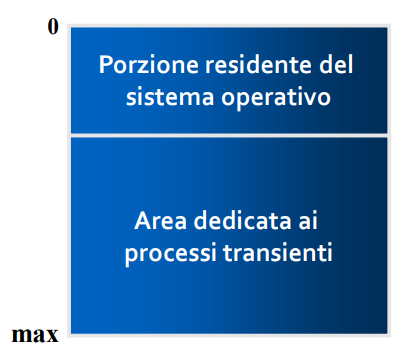
\includegraphics[width=0.50\textwidth]{Monoallocazione}
	\end{figure}
	\paragraph{Modalità dello schema}: \\
	Il sistema operativo effettua diversi compiti:
	\begin{itemize}
		\item tiene traccia solo della prima e dell'ultima locazione disponibile per i processi transienti;
		\item viene posto ad uno dei due estremi della memoria;
		\item ingloba i vettori di interrupt;
		\item altri suoi moduli temporanei vengono posti all'altra estremità della memoria. 
	\end{itemize}
	Alla richiesta di esecuzione di un programma, il sistema operativo:
	\begin{itemize}
		\item si assicura che le dimensioni del processo siano compatibili con la memoria disponibile;
		\item conferisce il controllo al processo utente fino al suo completamento o ad eventuali condizioni d'errore;
		\item al termine del processo la memoria viene liberata e può essere assegnata ad un altro processo in attesa.
	\end{itemize}
	\paragraph{Meccanismi di protezione} Raramente un monitor monoprocesso supporta meccanismi di protezione tra processi utente in quanto in ogni istante vi può essere al massimo un solo processo residente in memoria. Gli eventuali meccanismi di protezione si riferiscono alla protezione del codice del sistema operativo da eventuali sconfinamento del processo transiente in esecuzione. \\
	La protezione del sistema operativo dai processi utente è spesso effettuata tramite supporti hardware come:
	\begin{itemize}
		\item \textbf{registri barriera}: questi sono usati per tracciare un confine tra le aree dei processi di sistema e dei processi transienti. Nel registro viene salvata la prima locazione disponibile al processo in modo che il sistema operativo possa controllare un eventuale sconfinamento, per fare questo, però, ci deve essere la capacità di distinguere l'esecuzione del sistema operativo da quella dei processi utente definendo gli stati utente e supervisore;
		\item \textbf{diritti di accesso mediante bit di protezione}: con questo metodo ad ogni parola di memoria viene associato un bit di protezione che viene posto a 1 nelle zone che contengono il sistema operativo e a 0 nelle restanti, in questo modo i processi utente accedono solo a parole con bit 0, mentre il sistema operativo può accedere ovunque;
		\item \textbf{sistema operativo in memoria a sola lettura}: questo è un metodo semplice e diffuso che è scarsamente utilizzato nei personal computer in quanto poco flessibile e rende impossibile correggere o aggiornare il codice del sistema operativo.
	\end{itemize}
	La condivisione del codice e dei dati non ha senso negli ambienti monoprocesso e raramente viene supportata dai monitor. I programmi utente potrebbero passarsi dei dati, mediante accordi interni, ponendoli in locazioni di memoria che non vengono sovrascritte durante l'esecuzione dei processi partecipanti o mediante file.
	\paragraph{Prestazioni}:
	\begin{itemize}
		\item \textbf{Difetti:}
		\begin{itemize}
			\item la mancanza di supporti per la multi-programmazione produce un abbassamento dell'efficienza sia della memoria che della CPU;
			\item la memoria può risultare troppo grande per la maggioranza dei processi;
			\item processi di dimensioni più grandi non possono essere eseguiti, oppure richiedono la tecnica dell'\textbf{overlay} cioè richiedono particolari suddivisioni del codice;
			\item i programmi tendono ad essere ottimizzati rispetto alla dimensioni, comportando sacrifici di funzionalità e velocità (anche se adesso accade il contrario)
		\end{itemize}
		\item \textbf{Pregi:}
		\begin{itemize}
			\item basso costo di progettazione del modulo di gestione della memoria;
			\item contenuti supporti hardware specifici per la gestione della memoria.
		\end{itemize}
	\end{itemize}
	\subsection{Partizionamento statico}
	Un modo per supportare la multiprogrammazione consiste nel dividere la memoria in diverse partizioni, ciascuna delle quali può essere allocata a un processo diverso. \\
	IL partizionamento statico implica che la suddivisione della memoria venga fatta a priori e che da quel momento le partizioni rimangano di dimensioni fisse. \\
	Il numero e la dimensione di ciascuna partizione vengono determinato durante la generazione del sistema considerando alcuni fattori:
	\begin{itemize}
		\item capacità della memoria fisica disponibile;
		\item grado desiderato di multiprogrammazione;
		\item dimensione dei processi più frequentemente eseguiti.
	\end{itemize}
	Alcuni calcolatori permettono una ridefinizione manuale delle partizioni senza dover ripetere l'intero processo di generazione del sistema. \\
	\paragraph{Principi operativi}: \\
	Il sistema operativo deve tener traccia delle partizioni definite. Lo stato corrente delle partizioni e i loro attributi vengono raccolti in una struttura dati chiamata \textbf{tabella di descrizione delle partizioni o TDP}. \\
	L'unico campo della TDP che cambia è lo stato della partizione che indica se è allocata o meno, gli altri contengono valori definiti al momento del partizionamento. \\
	Segue un esempio di memoria partizionata:
	\begin{figure}[H]
		\centering
		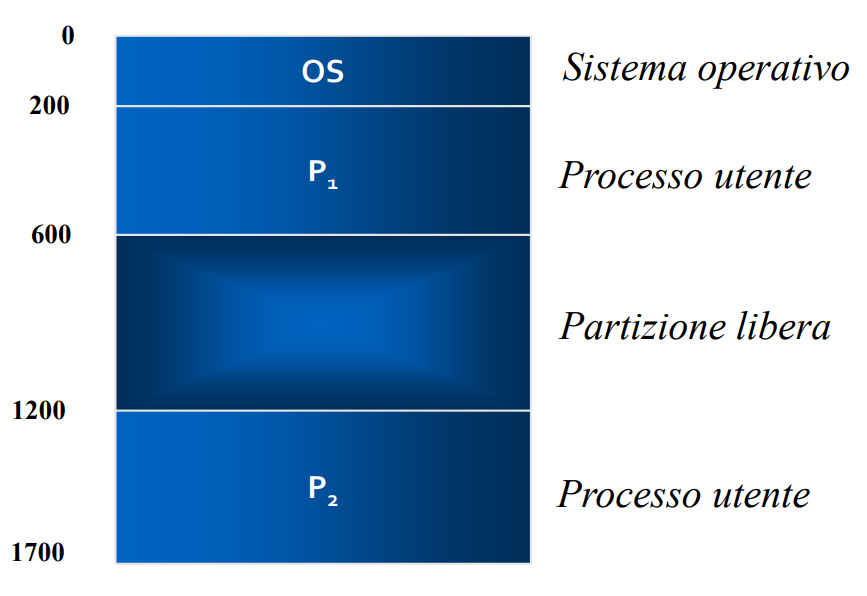
\includegraphics[width=0.75\textwidth]{Partizionamento_statico}
	\end{figure}
	La TDP dell'esempio precedente è: \\
	\begin{tabular}{|c | c | c | c|} 
		\hline
		\textbf{Numero partizione} & \textbf{Base partizione} & \textbf{Dimensione partizione} & \textbf{Stato partizione} \\
		\hline
		0 & 0 kB & 200 kB & Allocata \\
		\hline
		1 & 200 kB & 400 kB & Allocata \\
		\hline
		2 & 600 kB & 600 kB & Libera \\
		\hline
		3 & 1200 kB & 500 kB & Allocata \\
		\hline
	\end{tabular}
	Quando un processo non residente deve essere creato o attivato, il sistema operativo tenta di allocare una partizione di memoria libera di dimensioni sufficienti per contenerlo, consultando la TDP. Se il test è positivo, il campo che indica lo stato della partizione viene impostata ad "Allocata" e l'immagine del processo viene caricata nella corrispondente partizione. \\
	Quando il processo termina è necessario effettuarne uno swapping dalla memoria. Questa informazione verrà utilizzata per localizzare e aggiornare lo stato della partizione associata al valore "Libera". \\
	I metodi più comuni per la ricerca di una partizione libera sono:
	\begin{itemize}
		\item \textbf{First fit}: consiste nell'allocare la prima partizione libera sufficientemente larga per contenere il processo;
		\item \textbf{Best fit:} consiste nell'allocare la più piccola delle partizioni libere che contenga il processo
	\end{itemize}
	Il metodo first fit è più veloce in esecuzione perchè si arresta nella ricerca alla prima partizione libera disponibile, mentre il metodo best fit deve controllare tutte le partizioni libere disponibili e poi individuare quella migliore. Tuttavia, il metodo best fit è più accurato in esecuzione e quindi può raggiungere un migliori utilizzo della memoria, rispetto al metodo first fit, riducendo al minimo la differenza di dimensione tra il processo e la partizione allocata. Però, quando il numero di partizioni è elevato nessuno dei due metodi si rivela adatto.
	Quindi, per riassumere, se esiste una partizione allocabile al processo richiedente:
	\begin{itemize}
		\item l'allocazione viene effettuata;
		\item la TDP viene aggiornata;
		\item nel descrittore del processo si registra la partizione associata;
		\item quando il processo termina la partizione viene disallocata.
	\end{itemize}
	Le cause di mancata disponibilità di una partizione sono:
	\begin{enumerate}
		\item \textbf{non vi sono partizioni di memoria sufficientemente grandi per contenere il processo entrante} \\
		Le \textbf{cause} potrebbero essere:
		\begin{itemize}
			\item errore di scelta della dimensione delle partizioni;
			\item processo eccezionalmente più grande della norma.
		\end{itemize}
		La \textbf{soluzione} è di ridefinire le dimensioni delle partizioni, oppure il programma di origine deve essere progettato utilizzando uno schema di overlay;
		\item \textbf{tutte le partizioni sono allocate} \\
		In questo caso bisogna attendere una partizione libera oppure effettuare lo swapping del processo. \\
		Queste soluzioni possono essere applicate anche al caso 3;
		\item \textbf{alcune partizioni sono libere ma nessuna di esse è sufficientemente grande} \\
		In questo caso l'assegnazione delle partizioni può continuare. Vengono allocate partizioni a processi più piccoli, l'utilizzo della memoria viene mantenuto più elevato. Si può violare l'ordinamento di attivazione dei processi dallo scheduler modificando così, le prestazioni del sistema.
	\end{enumerate}
	Il funzionamento del gestore della memoria e dello scheduler sono strettamente correlati:
	\begin{itemize}
		\item lo scheduler determina quali processi sono pronti, e quindi residenti in memoria, in attesa della CPU
		\item il gestore della memoria può decidere di togliere un processo in memoria per liberare una partizione. 
	\end{itemize}
	\paragraph{Swapping}:
	Lo swapping è l'operazione di rimozione della memoria di un processo sospeso ed il suo successivo caricamento. Nel partizionamento statico questo aumenta il livello di occupazione della memoria centrale e di conseguenza il livello di utilizzo della CPU.	\\
	Quando lo scheduler decide l'introduzione in memoria di un nuovo processo il gestore dello swapping ne sceglie uno da rimuovere in base a:
	\begin{itemize}
		\item dimensione della partizione richiesta;
		\item priorità del processo;
		\item tipo di evento atteso dal processo;
		\item tempo già trascorso in memoria. 
	\end{itemize}
	Un processo residente in memoria, già parzialmente eseguito, è costituito da:
	\begin{itemize}
		\item codice eseguibile;
		\item dati finora elaborati;
		\item stack;
		\item registri di stato;
		\item file aperti;
		\item descrittore del processo.
	\end{itemize}
	Al momento dello swapping questi oggetti vengono registrati in un file su hard disk detto file di swapping. \\
	Tutti i processi che hanno subito uno swapping possono essere mantenuti in un file unico per tutto il sistema o in file separati, ciascuno assegnato ad un singolo processo. \\
	Un file di swapping viene solitamente creato al momento dell'inizializzazione del sistema e collocato su una periferica veloce di memorizzazione secondaria. L'indirizzo e la dimensione di tale file sono solitamente statici in modo da beneficiare di un indirizzamento diretto su disco. \\
	Un parametro critico per la realizzazione dei file di swapping è la dimensione:
	\begin{itemize}
		\item se troppo grande spreca spazio su dischi veloci;
		\item se troppo piccolo può rendere indisponibile l'operazione di swapping
	\end{itemize}
	L'alternativa è disporre di un file di swapping per ciascun processo presente nel sistema che può essere creato dinamicamente al momento della creazione del processo o staticamente al momento della preparazione del programma. In questo modo non vige più il problema della dimensione e non c'è nessuna restrizione sul numero di processi attivi. D'altra parte, però, c'è maggior spreco di spazio e maggiori tempi di accesso ai file distribuiti sul disco. \\
	Uno swapping efficiente richiede che i processi siano rilocabili dinamicamente:
	\begin{itemize}
		\item il processo può iniziare l'esecuzione in qualunque area di memoria;
		\item può essere spostato in un'altra area di memoria;
		\item il calcolo degli indirizzi effettuato dinamicamente ad esempio con l'uso di un \textit{registro base}
	\end{itemize}
	Processi non rilocabili dinamicamente sono legati alle partizioni in cui iniziano l'esecuzioni e rendono inefficiente lo swapping. Lo swapping va utilizzato solo in casi di necessità perchè la CPU spreca un tempo elevato nelle operazioni di trasferimento.
	\paragraph{Meccanismi di protezione}
	L'integrità di un sistema multiprogrammato dipende anche dalla sua capacità di garantire l'isolamento tra spazi di indirizzi separati. Non solo si deve proteggere il sistema operativo dai processi utente ma bisogna anche proteggere i processi utente tra di loro perchè nessuno possa invadere lo spazio riservato all'altro. \\
	Un sistema di protezione efficace non può prescindere dall'esistenza di un supporto hardware. Nei sistemi che utilizzano per la rilocazione i registri base, vengono usati di solito dei \textit{registri limite} per la protezione, il cui compito è di individuare i tentativi di accesso oltre i limiti dello spazio di indirizzamento assegnato al programma in esecuzione dal sistema operativo. Il registro limite contiene il valore dell'indirizzo virtuale più alto contenuto dal programma. \\
	Ad ogni accesso alla memoria alla CPU controlla che il programma non richieda gli indirizzi oltre il limite. Le violazione vengono rilevate e riferite al sistema operativo che le gestisce. L'indirizzo più basso del processo è contenuto nel registro base:
	\begin{figure}[H]
		\centering
		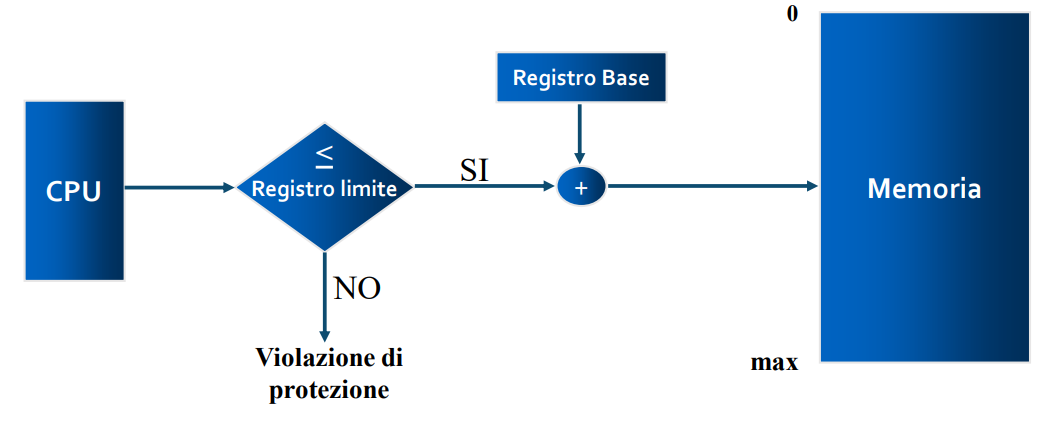
\includegraphics[width=1.00\textwidth]{Registri_limite}
	\end{figure}
	\paragraph{Meccanismi di condivisione} Un buon sistema di gestione della memoria deve occuparsi, oltre che della protezione, anche della condivisione controllata dei dati e codice tra processi cooperanti. I sistemi a partizioni fisse non sono adatti alla condivisione, poichè basano i propri meccanismi sull'isolamento degli spazi di indirizzamento. \\
	Alcuni possibili metodi di condivisione sono:
	\begin{enumerate}
		\item affidare gli oggetti condivisi al sistema operativo che così è in grado di accedere a tutte le risorse. Gli svantaggi di questa tecnica è che l'area del sistema operativo dovrebbe poter variare dinamicamente e le routine dei processi devono essere linkate al sistema operativo dinamicamente;
		\item ogni processo possiede una copia identica dell'oggetto condiviso, che usa e diffonde gli aggiornamenti. Il problema di questa tecnica è che se il sistema supporta lo swapping, uno o più processi potrebbero non essere in memoria e quindi non essere pronti a ricevere gli aggiornamenti.
		\item Collocare i dati in una partizione comune dedicata. In questo caso, però, il sistema operativo considera come violazione i tentativi dei processi di accedere a zone di memoria esterne alle rispettive partizioni. Se il sistema utilizza registri base e limite sono necessari accorgimenti per indirizzare partizioni che potrebbero essere non contigue.
	\end{enumerate}
	\paragraph{Conclusioni}:
	Il partizionamento statico è uno dei metodi più semplici di gestione della memoria, pur supportando la multiprogrammazione; richiede un hardware modesto e si adegua ad ambienti statici con carico predicibile di lavoro come ambienti dove vengono eseguiti solo applicativi, controllo di processi e sistemi di tipo bancario. \\
	Il problema principale è la \textbf{frammentazione interna}, inoltre, può richiedere progettazione dei programmi con schemi ad overlay; non si adatta a contenere oggetti come stack che possono crescere in maniera non facilmente controllabile e il numero di partizioni fissato limita il grado di multiprogrammazione. \\
	La \textbf{frammentazione interna} si verifica quando una partizione di memoria assegnata a un processo è più grande di quanto richiesto dal processo stesso. Questo crea dello spazio inutilizzato all'interno della partizione, che non può essere utilizzato da altri processi e quindi la memoria allocata viene in parte "sprecata" perchè non viene completamente utilizzata.
	\subsection{Partizionamento dinamico}
	Il sistema delle partizioni è analogo a quello del partizionamento statico.
	Il gestore della memoria crea ed assegna partizioni di \textbf{dimensioni variabili dinamicamente} in base alla richieste dei processi.
	Quando un processo termina o subisce uno swapping, il gestore della memoria restituisce lo spazio liberato all'insieme di aree di memoria libere. Il gestore della memoria può creare e allocare partizioni finchè non viene esaurita la memoria fisica o finchè non viene raggiunto il massimo grado di multiprogrammazione.
	\paragraph{Principi operativi}:\\
	Alla richiesta di una partizione il gestore della memoria (GM) ricerca una zona di memoria libera contigua di dimensione sufficiente. Se si trova un'area adatta il sistema operativo vi ricava una partizione in modo da soddisfare esattamente le necessità del processo. \\
	L'eventuale parte rimanente di memoria libera viene restituita all'insieme della memoria libera e posta a disposizione del modulo di allocazione. La partizione viene creata registrando la sua base, la sua dimensione e il suo stato nella TDP. 
	Alcune di queste informazioni vengono anche registrate nel descrittore di processo. Dopo aver caricato l'immagine del processo nella partizione creata, il processo viene sottoposto al controllo di un modulo del sistema operativo che si occupa delle operazioni successive. \\
	Quando un processo termina o subisce uno swapping il sistema operativo restituisce la partizione all'area libera e cancella la riga nella TDP. L'insieme delle aree libere varia dinamicamente, gli spazi interni all'area libera vengono utilizzati per mantenere una lista a puntatori. Ad esempio: 
	\begin{figure}[H]
		\centering
		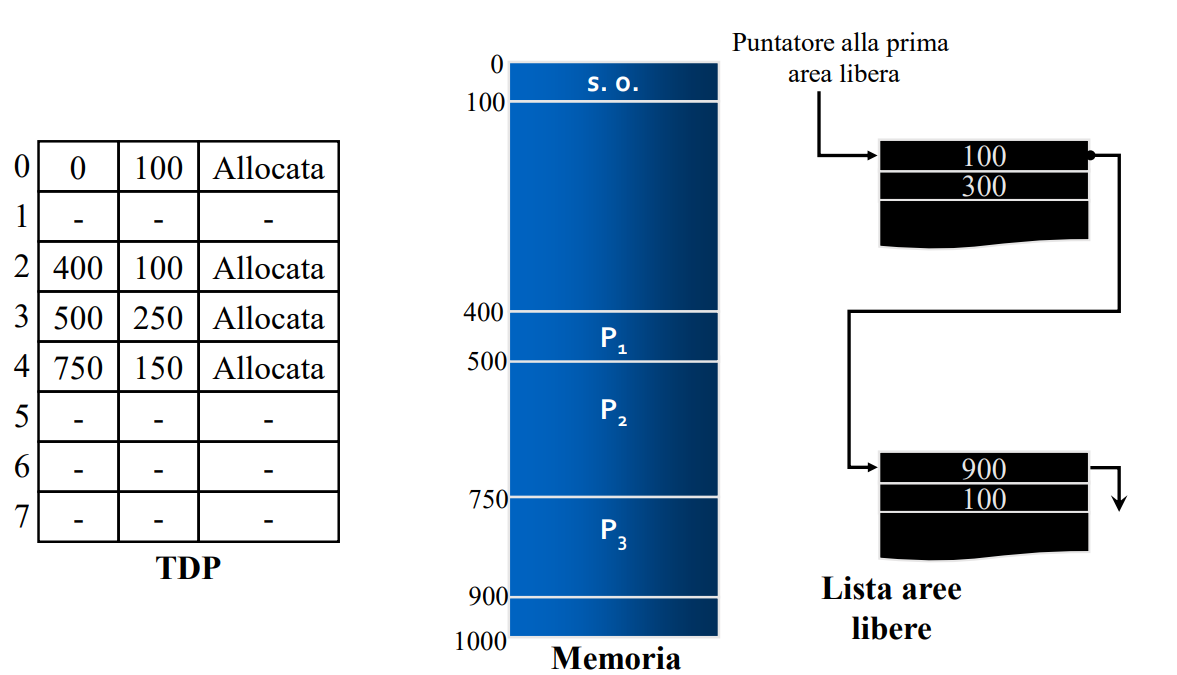
\includegraphics[width=0.70\textwidth]{partizionamento_dinamico}
	\end{figure}
	Gli algoritmi più comuni per selezionare un'area di memoria all'interno della quale creare una partizione sono:
	\begin{itemize}
		\item \textbf{First-fit}: questo metodo termina la ricerca quando viene individuato il primo blocco di memoria sufficientemente grande da contenere il processo;
		\item \textbf{Next-fit}: questo metodo è una variante del First-fit. In questo metodo il puntatore alla lista delle aree libere, dopo aver effettuato un'allocazione, viene salvato cosicchè la ricerca successiva continua da dove si era fermata la precedente;
		\item \textbf{Best-fit}: questo metodo alloca il blocco di memoria più piccolo che può contenere il processo;
		\item \textbf{Worst-fit}: questo metodo alloca il blocco di memoria più grande le cui dimensioni superino quella della partizione richiesta.
	\end{itemize}
	\paragraph{Compattazione} Lo schema di partizionamento dinamico genera dei buchi di memoria inutilizzabile e questo è inevitabile. Per questo motivo può anche diventare impossibile l'allocazione di una memoria richiesta da un processo, pur contenendo la memoria globalmente un'area di dimensione sufficiente. Questo problema prende il nome di \textbf{frammentazione esterna}. \\
	Quando la frammentazione raggiunge un grado elevato è necessario effettuare la \textbf{compattazione della memoria} che consiste nello spostare i processi residenti in memoria in modo da creare partizioni libere più grandi. Questa operazione richiede un grande costo di CPU. \\
	La compattazione può essere effettuata:
	\begin{itemize}
		\item \textbf{Continuamente:}
		\begin{itemize}
			\item la memoria viene compattata ogni volta che un processo libera un'area;
			\item la frammentazione è ridotta al minimo;
			\item questa operazione ha un grande costo di CPU.
		\end{itemize}
		\item \textbf{Su necessità:}
		\begin{itemize}
			\item la compattazione viene effettuata quando non si riesce ad allocare memoria ad un processo richiedente;
			\item un controllo preliminare verifica se il totale dell'area liberabile è sufficiente a contenere il processo.
		\end{itemize}
	\end{itemize}
	La compattazione può essere effettuata in due modi:
	\begin{enumerate}
		\item \textbf{Spostamento selettivo incrementale:}
		\begin{itemize}
			\item ricerca di una strategia ottima di movimento per compattare al meglio la memoria;
			\item consente di risparmiare tempo negli spostamenti;
			\item poco utilizzata perchè richiede un sovraccarico notevole
		\end{itemize}
		\item \textbf{Spostamento globale:}
		\begin{itemize}
			\item tutte le partizioni vengono rilocate ad uno dei due estremi della memoria;
			\item il tempo di trasferimento delle partizioni non è ottimizzabile;
			\item non richiede strategie particolari.
		\end{itemize}
	\end{enumerate}
	Segue un esempio di spostamento selettivo e globale:
	\begin{figure}[H]
		\centering
		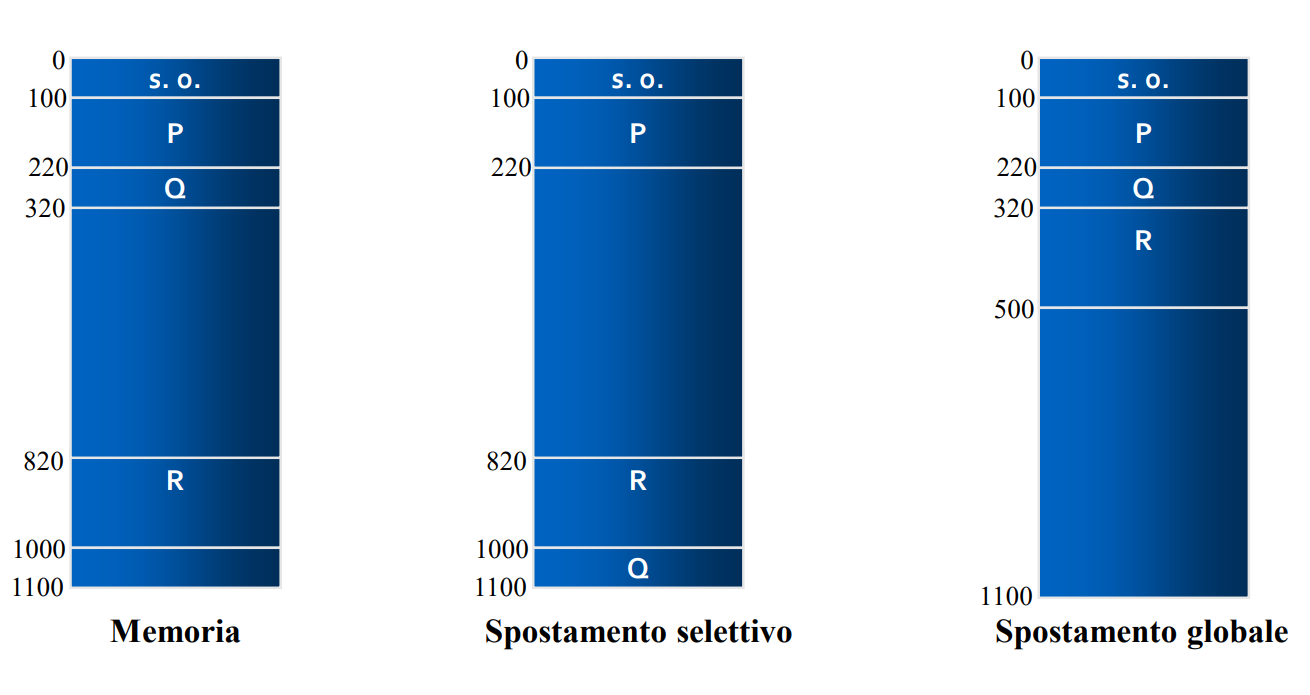
\includegraphics[width=1.00\textwidth]{compattazione}
	\end{figure}
	\paragraph{Meccanismi di protezione e condivisione} Le tecniche di protezione e condivisione sono analoghe a quelle del partizionamento statico, considerato che il supporto hardware è simile. Nel partizionamento dinamico è possibile una particolare forma di condivisione:
	\begin{itemize}
		\item a due partizioni contigue è consentito sovrapporsi, mettendo un'area in comune;
		\item questa forma di condivisione è molto restrittiva, in quanto, può avvenire solo tra due processi.
	\end{itemize}
	\paragraph{Conclusioni} Il partizionamento dinamico:
	\begin{itemize}
		\item richiede un sopporto hardware modesto, analogo al partizionamento statico;
		\item la differenza tra i due schemi risiede sostanzialmente nel software;
		\item elimina la frammentazione interna ma produce quella esterna che può essere eliminata con la compattazione;
		\item si adegua ad ambienti con carico non predicibile di lavoro come ad esempio sviluppo di software.
	\end{itemize}
	\subsection{Segmentazione}
	La segmentazione è uno schema di gestione della memoria che si basa sulla divisione dello spazio di indirizzamento dei processi in entità logiche che possono essere poste in aree non contigue di memoria. La segmentazione fornisce strumenti per la rilocazione dinamica, la protezione e la condivisione. \\
	La frammentazione esterna può essere ridotta se la dimensione delle aree richieste è più piccola. Un programma eseguibile può essere diverso, ad esempio, in codice, dati e stack; ciascuno di questi oggetti può essere posto in un segmento diverso di dimensioni differenti. \\
	La segmentazione condivide alcune proprietà con gli altri schemi di allocazione di memoria, in particolare:
	\begin{itemize}
		\item degli \textbf{schemi di allocazione contigua} relativamente ad un singolo elemento, poichè i dati di ogni singola entità logica devono essere posti in un'area contigua di memoria;
		\item degli \textbf{schemi di allocazione non contigua} relativamente all'intero spazio di indirizzamento del processo, poichè i blocchi logici diversi possono essere messi in segmenti non contigui.
	\end{itemize}
	\paragraph{Principi operativi} La raccolta degli oggetti in segmenti viene effettuata dal programmatore. Ciascun segmento inizia all'indirizzo virtuale 0. Ogni segmento ha un nome che viene poi tradotto in un indirizzo in fase di caricamento della memoria e un singolo dato all'intero del segmento viene identificato dallo spiazzamento relativo all'inizio del segmento a cui appartiene.\\
	L'indirizzamento nella segmentazione è di tipo bidimensionale, infatti la designazione univoca di un dato o di una istruzione richiede il nome del segmento e lo spiazzamento all'interno del segmento. La memoria fisica, mantiene l'indirizzamento lineare, per cui gli indirizzi bidimensionali di segmenti virtuali devono essere tradotti in indirizzi fisici. \\
	Il caricamento di un processo segmentato avviene nel seguente modo:
	\begin{itemize}
		\item il Sistema Operativo cerca di allocare $n$ partizioni adatte per gli $n$ segmenti in cui è suddiviso il processo;
		\item il Sistema Operativo crea un descrittore di segmento registrandovi l'indirizzo fisico in cui è stato posto il segmento e la sua dimensione;
		\item l'insieme dei descrittori di segmento di un processo viene raccolto nella tabella dei descrittori di segmento o \textbf{TDS}.
	\end{itemize}
	La conversione di un indirizzo avviene nel seguente modo:
	\begin{itemize}
		\item l'indirizzo bidimensionale virtuale, formato dal nome del segmento e dallo spiazzamento, è tradotto in modo equivalente al meccanismo del registro base;
		\item il segment viene utilizzato per ritrovare l'indirizzo fisico del segmento nella TDS;
		\item il displacement viene sommato all'indirizzo fisico del segmento per ottenere l'indirizzo fisico richiesto;
		\item la dimensione del segmento, riportata nella TDS, viene anche utilizzata per controllare eventuali violazioni.
	\end{itemize}
	Segue un'immagine esplicativa riguardante la traduzione degli indirizzi:
	\begin{figure}[H]
		\centering
		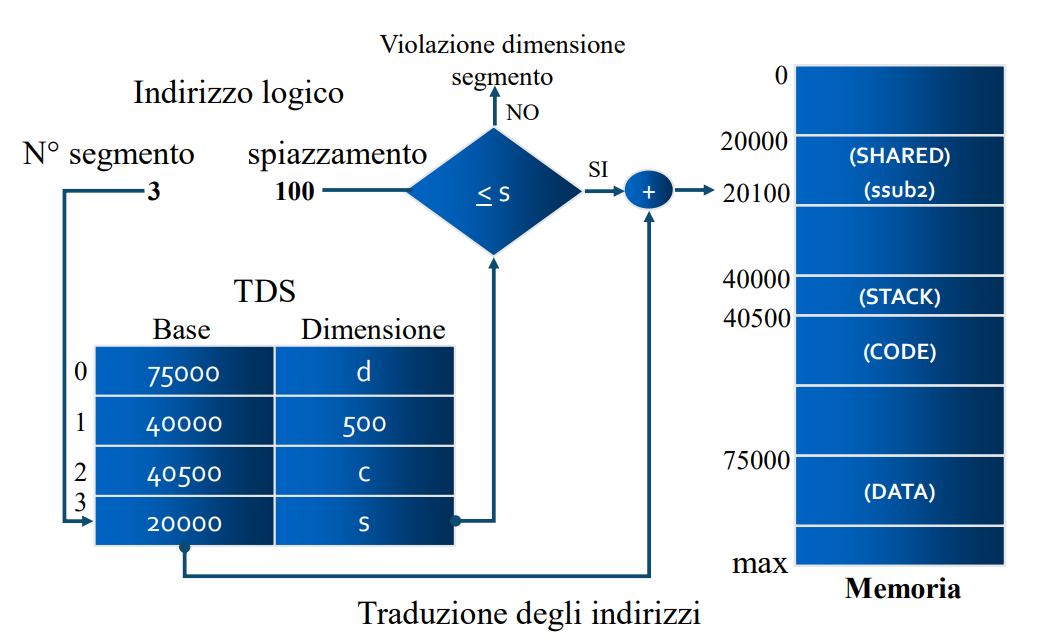
\includegraphics[width=1.00\textwidth]{segmentazione}
	\end{figure}
	Le dimensioni della TDS sono legate alle dimensioni dello spazio virtuale di indirizzamento di uj processo. I processori della famiglia Intel, supportano fino a 16000 segmenti di 64 kb. La TDS può essere costituita da qualche riga fino a migliaia di righe e viene tenuta in memoria in uno dei segmenti associati al processo. \\
	Due registri hardware, \textbf{RBTDS} e \textbf{RLTDS}, contengono l'indirizzo di inizio e fine della TDS associata al processo in esecuzione e questo consente anche il controllo d'accesso a segmenti non assegnati al processo. 
	\begin{itemize}
		\item \textbf{RBTDS}: Registro Base della Tabella dei Descrittori di Segmento;
		\item \textbf{RLTDS}: Registro Limite della Tabella dei Descrittori di Segmento.
	\end{itemize}
	Quindi, la base ed il limite della nuova TDS vengono caricati nei registri RBTDS e RLTDS. Quando un processo subisce uno swapping, al ritorno in memoria va aggiornata la sua TDS anche se generalmente si preferisce rigenerarla totalmente utilizzando la mappa statica fornita dal linker. L'eventuale compattazione richiede l'aggiornamento nella TDS delle righe relative ai segmenti spostati. \\
	La traduzione di ciascun indirizzo bidimensionale virtuale richiede due accessi in memoria:
	\begin{itemize}
		\item uno alla TDS per tradurre l'indirizzo del segmento da virtuale a fisico;
		\item l'altro per accedere fisicamente alla locazione richiesta.
	\end{itemize}
	La segmentazione, quindi, raddoppia il tempo per l'accesso ad una locazione di memoria. \\
	Se i descrittori di segmento sono pochi, o se alcuni sono utilizzati frequentemente, conviene specificare il loro caricamento in opportuni registri hardware. I processori della famiglia Intel, dispongono di 4 registri utilizzabili da schemi di segmentazione e sono:
	\begin{itemize}
		\item \textbf{CS: Code Segment};
		\item \textbf{SS: Stack Segment};
		\item \textbf{DS: Data Segment};
		\item \textbf{ES: Extra Segment}.
	\end{itemize}
	\paragraph{Meccanismi di protezione}
	La segmentazione è lo schema migliore per quanto riguarda i meccanismi di protezione e anche di condivisione. \\
	La forma più naturale di protezione per un sistema segmentato è l'utilizzo di registri base e limite. La protezione tra spazi di indirizzamento di processi differenti è garantita dalla collocazione dei segmenti in aree disgiunte di memoria. Una caratteristica offerta dai sistemi segmentati consiste nel fornire un livello di protezione all'interno dello spazio di indirizzamento di un singolo processo. \\
	Infatti, è possibile definire diritti e modalità di accesso per ogni tipo di segmento. Ad esempio:
	\begin{itemize}
		\item accesso in modalità \textit{execute} o \textit{read-only} al segmento codice;
		\item accesso in modalità \textit{read/write} al segmento stack;
		\item accesso \textit{read-only} o \textit{read/write} al segmento dati.
	\end{itemize}
	I diritti di accesso possono essere registrati in un campo della TDS.
	\paragraph{Meccanismi di condivisione}
	La segmentazione offre una condivisione semplice e flessibile. Gli oggetti condivisi sono collocati in segmenti dedicati e separati. Il segmento condiviso può essere mappato attraverso la TDS, nello spazio di indirizzamento virtuale di tutti i processo che hanno il permesso di accedervi e questo è possibile dato che lo spiazzamento interno di un dato è identico per tutti i processi che lo condividono dato che i segmenti iniziano con un indirizzo virtuale pari a 0. \\
	Segue un esempio di meccanismi di condivisione tra processi:
	\begin{figure}[H]
		\centering
		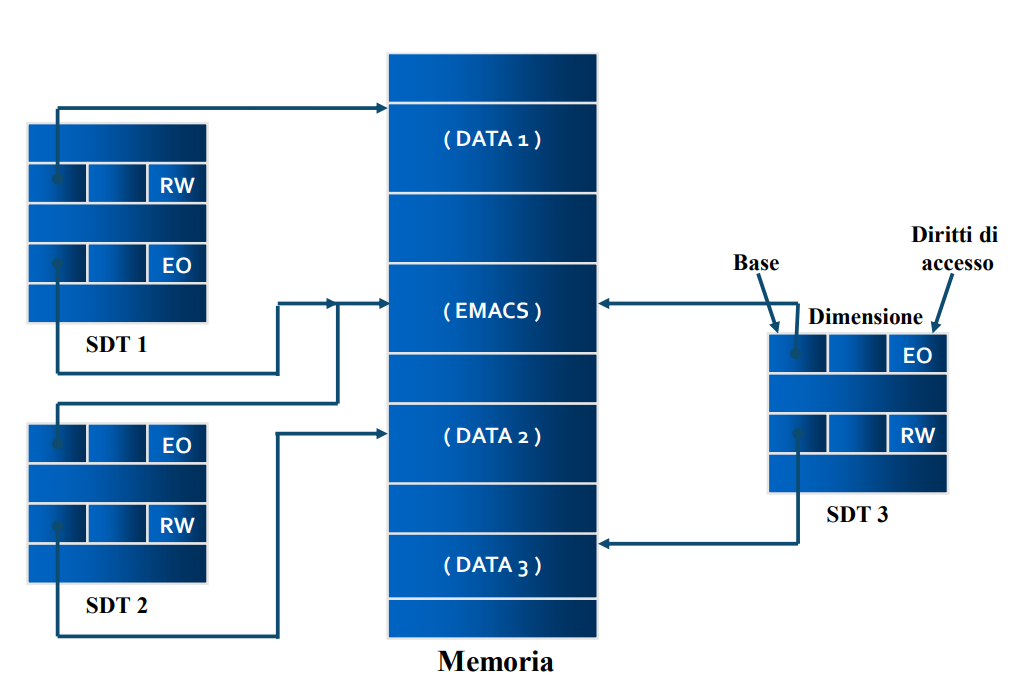
\includegraphics[width=1.00\textwidth]{meccanismi_condivisione_segmentazione}
	\end{figure}
	\paragraph{Collegamento dinamico} Il \textbf{collegamento dinamico} indica il caricamento di una procedura, come una libreria, in fase di esecuzione di un processo e solo su sua richiesta. Lo spazio in memoria per una procedura viene occupato solo quando questa viene richiesta. La segmentazione consente di aggiungere nuovi segmenti al processo richiedente, aggiornando la TDS e i registri base e limite della TDS.
	\paragraph{Conclusioni}
	La gestione della memoria fisica è più efficiente perchè non c'è più la necessità di allocare i processi in aree contigue. Inoltre, con la segmentazione la frammentazione interna è pari a 0, la frammentazione esterna è ridotta al minimo, come detto in precedenza la segmentazione è lo schema migliore per quanto riguarda i meccanismi di condivisione e di protezione e inoltre, la segmentazione fornisce una funzionalità utile, cioè quella del \textbf{linking dinamico}. \\
	Gli svantaggi principali che derivano dall'uso di questo schema sono diversi. Innanzitutto, vige la necessità di effettuare la compattazione che è più complessa. Inoltre, il duplice accesso alla memoria deve essere supportato da un hardware apposito, la gestione della memoria da parte del sistema operativo è più complessa rispetto a quella per il partizionamento statico e dinamico e non c'è ancora la possibilità di eseguire processi più grandi delle dimensioni fisiche della memoria.
	\section{Allocazione non contigua}
	\subsection{Paginazione}
	Nella paginazione la memoria fisica viene concettualmente suddivisa in pagine di dimensione fissa chiamate \textbf{pagine fisiche} e anche lo spazio di indirizzamento dei processi viene diviso in \textbf{pagine virtuali} della stessa dimensione delle pagine fisiche. \\
	Il meccanismo di traduzione fa corrispondere indirizzamenti all'interno di pagine virtuali ad indirizzamenti in pagine fisiche e ogni pagina è mappata separatamente quindi non è necessaria la contiguità delle pagine fisiche. \\
	Nella paginazione la frammentazione esterna sparisce mentre la frammentazione interna è molto piccola che è al più un byte per processo.
	\paragraph{Principi operativi} Ogni indirizzo all'interno di un processo è diviso in:
	\begin{itemize}
		\item bit più significativi che corrispondono al numeri di pagina virtuale;
		\item bit meno significativi che corrispondono allo spiazzamento reale.
	\end{itemize}
	Il sistema operativo tiene traccia della corrispondenza tra pagine virtuali e pagine fisiche mediante la \textbf{tabella delle pagine o TDP}. 
	La TDP viene costruita al momento del caricamento del processo, ogni riga della tabella contiene l'indirizzo di partenza della pagina fisica in cui è allocata la corrispondente pagina virtuale e ne vengono salvati solo i bit più significativi e la tabella è costituita da un numero di righe pari al numero di pagine occupate. \\
	Ad esempio, supponiamo di avere una memoria di un 1 MB, suddivisa in 4096 pagine della dimensione di 256 byte ciascuna e con una lunghezza di indirizzo di 20 bit. Lo spazio di indirizzamento di un ipotetico processo utente che occupa 1008 byte (3F0H) viene suddiviso in quattro pagine virtuali da 0 a 3, in quanto quattro pagine permettono la memorizzazione di un processo di al massimo 1048 byte. \\
	La \textbf{traduzione} dell'indirizzo virtuale avviene nel seguente modo:
	\begin{itemize}
		\item un meccanismo hardware divide l'indirizzo virtuale in:
		\begin{itemize}
			\item 12 bit più significativi che indicano il numero di pagina;
			\item 8 bit meno significativi che indicano lo spiazzamento all'interno della pagina.
		\end{itemize}
		\item il numero di pagina viene usato all'interno della TDP per ottenere il corrispondente indirizzo della pagina fisica;
		\item l'indirizzo ottenuto, concatenato con il displacement, fornisce l'indirizzo fisico cercato.
	\end{itemize}
	\begin{figure}[H]
		\centering
		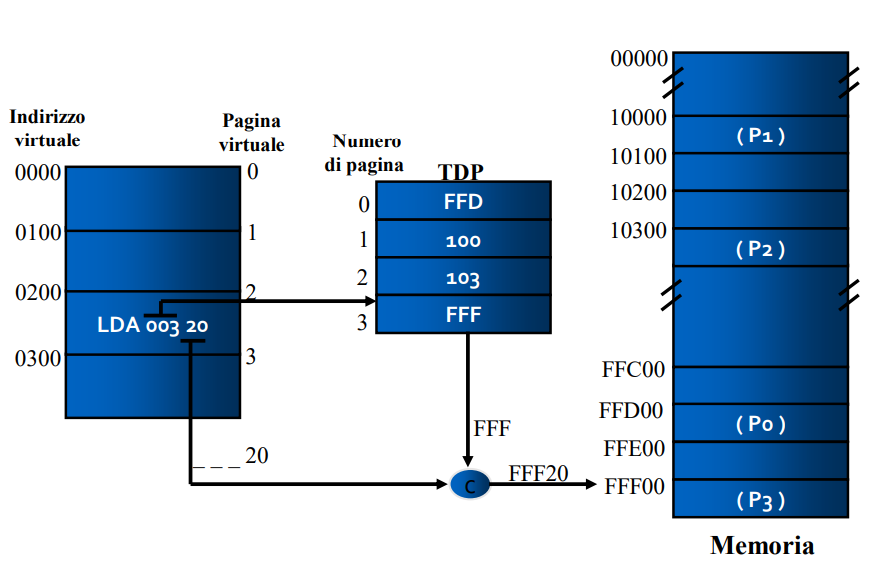
\includegraphics[width=1.00\textwidth]{paginazione}
	\end{figure}
	Il sistema operativo tiene traccia dello stato di tutte le pagine fisiche mediante la tabella di memoria, la TDM:
	\begin{itemize}
		\item in ogni riga della TDM è indicato lo stato della relativa pagina se libera o allocata;
		\item il numero di righe della tabella è uguale al numero di pagine fisiche.
	\end{itemize}
	\begin{figure}[H]
		\centering
		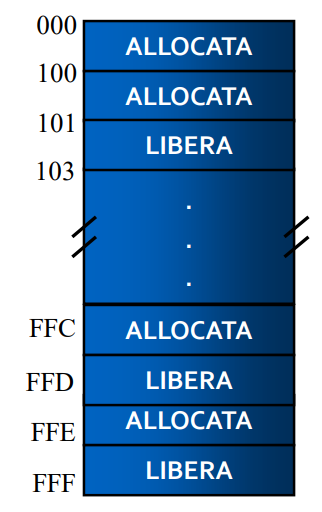
\includegraphics[width=0.50\textwidth]{tabella_di_memoria}
	\end{figure}
	Quando un processo termina o subisce uno swapping:
	\begin{itemize}
		\item restituisce tutte le pagine fisiche ad esso assegnate;
		\item la sua TDP viene eliminata.
	\end{itemize}
	Quando il processo richiedente ha uno spazio di indirizzamento non multiplo delle pagine fisiche si crea il fenomeno della \textit{frammentazione interna} della pagina ma questo è un fenomeno ridotto e legato alla dimensione della pagina fisica. \\
	Bisogna prestare attenzione, alla scelta della tecnica di \textbf{memorizzazione delle aree libere}, infatti, la consultazione della TDM statica per trovare $n$ pagine fisiche libere richiede una ricerca su un numero di righe in media $x = \dfrac{n}{q}$, dove $n$ corrisponde al numero di pagine libere che si vuole cercare e $q$ è la probabilità che una pagina sia libera ed è legata alla percentuale di memoria libera $u$, da questo segue che $q = \dfrac{u}{100} \quad 0 < q < 1$, quindi $x$ aumenta con l'aumentare della memoria utilizzata. Ad esempio: \\
	\[
	n = 10 \quad u = 40\% \quad q = 0.4 
	\]
	$x$ in media è di 25 righe per ritrovare 10 pagine libere. Da qui deduciamo che la consultazione della TDM non è particolarmente efficiente, soprattutto nel caso in cui la memoria è satura e quindi si tende a sostituire la TDM con una lista a puntatori contenente i numeri delle pagine fisiche:
	\begin{itemize}
		\item $n$ pagine da allocare si individuano nei primi $n$ nodi della lista;
		\item in fase di disallocazione vengono inseriti in testa alla lista gli $n$ nodi relativi alle pagine liberate.
	\end{itemize}
	Utilizzando questa tecnica il tempo di allocazione e disallocazione non dipende dalla percentuale di occupazione della memoria, però per il singolo elemento c'è un lieve spreco di memoria e di tempo rispetto alla gestione di una tabella statica.
	\paragraph{Cache di traduzione}: \\
	\begin{figure}[H]
		\centering
		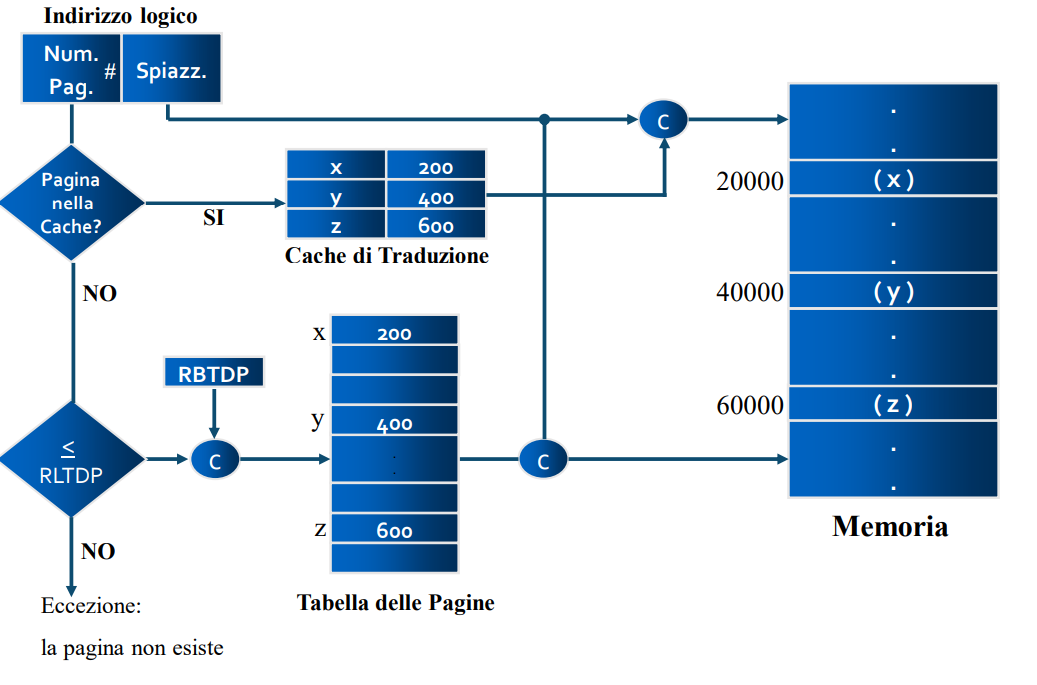
\includegraphics[width=1.00\textwidth]{cache_traduzione}
	\end{figure}
	\paragraph{Principi operativi} I meccanismi hardware per la paginazione vengono utilizzati per due scopi:
	\begin{enumerate}
		\item \textbf{Risparmiare la memoria necessaria per le TDP};
		\item \textbf{Velocizzare la traduzione da indirizzi virtuali a fisici}.
	\end{enumerate}
	\textbf{1. Risparmiare la memoria necessaria per le TDP}. \\
	Durante la costruzione delle tabelle delle pagine è giusto pensare di costruirle con un numero di righe uguale alle pagine effettivamente utilizzate. \\
	Di conseguenza, è necessario l'utilizzo di due registri hardware:
	\begin{itemize}
		\item registro \textbf{limite} della tabella TDP, \textbf{RLTDP} che contiene il numero di pagina virtuale più alto utilizzato dal processo;
		\item registro \textbf{base} della tabella TDP, \textbf{RBTDP} che contiene l'indirizzo di partenza della TDP.
	\end{itemize}
	I valori di questi due registri solitamente sono memorizzati nel descrittore di processo e questo meccanismo consente anche il controllo di accesso a pagine non assegnate al processo, vedi infatti l'esempio della cache di traduzione. \\
	\textbf{2. Velocizzazione del tempo di traduzione}. \\
	La traduzione di ciascun indirizzo virtuale richiede due accessi in memoria:
	\begin{itemize}
		\item uno alla TDP per prelevare il numero di pagina fisica;
		\item l'altro per accedere fisicamente alla locazione fisica.
	\end{itemize}
	Quindi la paginazione raddoppia il tempo per l'accesso ad una locazione di memoria e un metodo di velocizzazione è l'uso di una cache di traduzione che memorizza gli indirizzi delle pagine usate più frequentemente.
	\paragraph{Meccanismi di protezione}
	Nella paginazione la protezione interna viene meno rispetto alla segmentazione, questo perchè nella segmentazione era il programmatore a dividere il processo e stabiliva quali parti rendere solo leggibili o meno, mentre nella paginazione la divisione del programma viene effettuata dal sistema operativo e in una pagina è probabile trovare, ad esempio, pezzi di codice con pezzi di stack e quindi è difficile stabilire quale pagine rendere solo leggibile o meno. \\
	Gli spazi di indirizzamento distinti vengono di norma allocati in zone disgiunte della memoria e gli accessi alla memoria sono ristretti al proprio spazio di indirizzamento. \\
	Il registro limite della TDP blocca i tentativi di accedere a pagine virtuali oltre il limite assegnato al processo e i valori dei registri sono modificati esclusivamente da istruzioni privilegiate del sistema operativo.
	\paragraph{Meccanismi di condivisione}
	La condivisone è immediata con lo schema di paginazione, infatti:
	\begin{itemize}
		\item una copia unica di una pagina fisica può essere mappata in molti spazi di indirizzamento;
		\item i diversi processi possono avere un tipo di accesso diverso alla pagina;
		\item la condivisione viene riconosciuta ed effettuata da programmi di sistema, poichè la paginazione è trasparente all'utente;
		\item il codice condiviso deve essere naturalmente essere rientrante, cioè che non si automodifica e le variabili, costanti e stack sono raggruppati in aree separate. Un'alternativa al codice rientrante è di eseguire il codice condiviso in mutua esclusione
	\end{itemize}
	\subsection{Memoria virtuale}
	La memoria virtuale viene anche chiamata paginazione su richiesta o segmentazione su richiesta quindi si rifa alle tecniche di gestione della memoria o della paginazione o della segmentazione. \\
	La memoria virtuale è uno schema di gestione della memoria in cui soltanto una parte dello spazio di indirizzamento virtuale di un processo residente viene effettivamente caricata in memoria. \\
	Con questo tipo di gestione si ha che:
	\begin{itemize}
		\item la somma di tutti gli spazi di indirizzamento virtuali dei processi attivi può superare la capacità della memoria fisica;
		\item la dimensione ammissibile per lo spazio di indirizzamento virtuale di un singolo processo può superare la capacità della memoria fisica disponibile di un sistema.
	\end{itemize}
	Gli schemi dei precedenti tipi di gestione della memoria tendevano ad una occupazione della memoria vicina al 100\% mentre lo schema con memoria virtuale sembra fornire un grado di occupazione superiore al 100\%. \\
	Questo risultato si ottiene:
	\begin{itemize}
		\item mantenendo in memoria secondaria l'immagine dell'intero spazio virtuale di indirizzamento del processo;
		\item trasferendo in memoria fisica soltanto alcune parti al momento in cui sono necessarie;
		\item il sistema operativo sceglie tempi e modalità di trasferimento in memoria fisica tenendo conto di fattori quali:
		\begin{itemize}
			\item richieste dei processi attivi;
			\item priorità dei processi;
			\item disponibilità globali del sistema.
		\end{itemize}
	\end{itemize}
	Dal punto di vista del \textbf{programmatore}:
	\begin{itemize}
		\item i dettagli della gestione sono trasparenti;
		\item non è necessario l'adeguamento di un programma ad una memoria limitata;
		\item un programma può essere eseguito su sistemi con disponibilità di memoria fisica diversa, senza alcun adattamento.
	\end{itemize}
	Dal punto di vista del \textbf{sistema operativo:}
	\begin{itemize}
		\item un processo può essere caricato in uno spazio di dimensione arbitraria;
		\item si riduce la frammentazione esterna;
		\item non è necessario modificare l'ordine previsto di esecuzione di un processo;
		\item il quantitativo di memoria assegnato a un processo può variare durante la sua esecuzione;
		\item il sistema operativo può scegliere dinamicamente di velocizzare l'esecuzione di un processo allocando un quantitativo maggiore di memoria o, in alternativa, aumentare il grado di multiprogrammazione.
	\end{itemize}
	Bisogna fare alcune osservazioni. Un'istruzione può essere completata se quanto gli è necessario, cioè codice, stack e dati sono presenti in memoria. Se un processo richiede un oggetto fuori dalla memoria viene sospeso per un tempo relativamente lungo. \\
	L'importanza dell'uso dello schema di memoria virtuale si basa su alcune osservazioni:
	\begin{itemize}
		\item durante una specifica esecuzione, alcune parti del programma non vengono indirizzate;
		\item le diverse condizioni interne o esterne causano diversi tracciati ad ogni esecuzione di un processo;
		\item alcune parti di un programma vengono eseguite molto raramente come la routine di gestione degli errori;
		\item alcuni programmi contengono tracciati complementari, come i compilatori.
	\end{itemize}
	\paragraph{Principi operativi}
	Il funzionamento della memoria virtuale è analogo alla paginazione ed alla segmentazione e quindi con l'uso di tabelle di traduzione, la differenza  che alcune pagine possono non esserci e quindi essere mancanti e quindi il processo di conversione è più complesso. \\
	Il meccanismo di traduzione deve realizzare la funzione $f$ che associa i nomi virtuali alle locazioni fisiche e deve restituire $r$ se l'oggetto $x$ è in memoria reale alla locazione $r$, in caso contrario deve restituire una condizione critica.
	\paragraph{Tabelle}
	Lo schema di memoria virtuale fa uso della tabella di traduzione delle pagine, nel caso di memoria virtuale con schema a paginazione, con aggiunta di 1 bit di presenza che segnala se questa è in memoria o 0 se è una pagina mancante, cioè una \textbf{page fault}. \\
	Quando bisogna caricare un processo il sistema operativo crea la TDP, ponendo a 1 bit di presenza delle pagine portate in memoria. Se viene richiesta, successivamente, una pagina mancante il processo viene sospeso in attesa del suo caricamento e gli altri processi nel frattempo vengono eseguiti. \\
	Lo schema di memoria virtuale fa uso anche della \textbf{tabella di descrizione del file, TDF} che associa al numeri di pagine virtuali l'indirizzo di residenza di queste sulla memoria secondaria. 
	\begin{figure}[H]
		\centering
		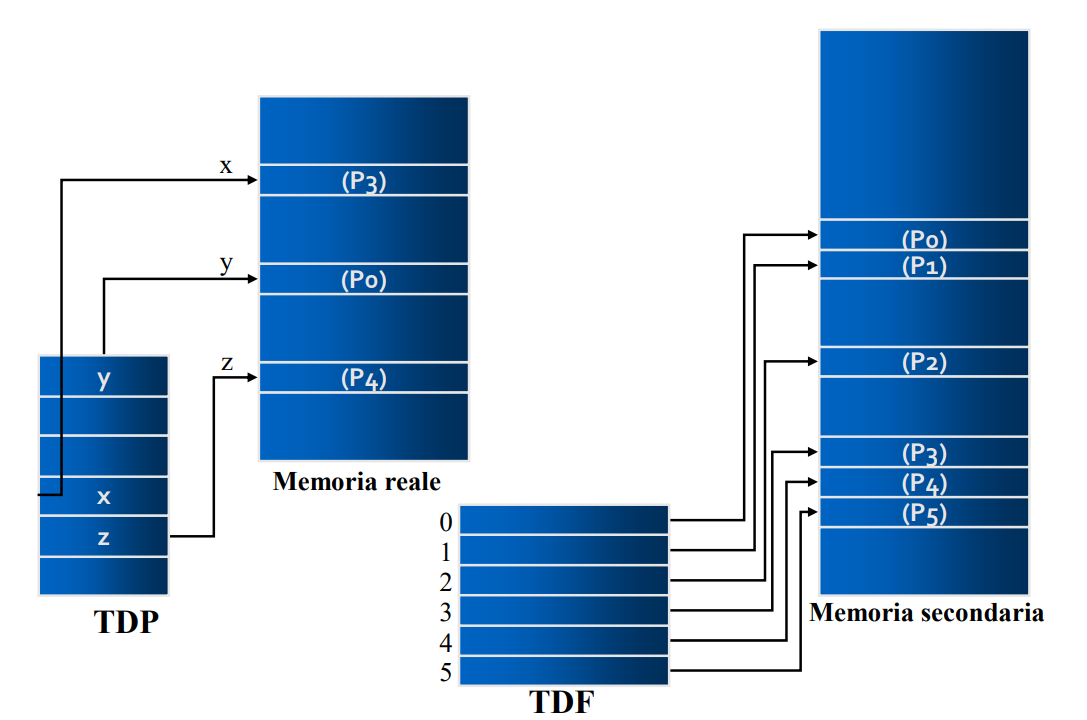
\includegraphics[width=1.00\textwidth]{tabelle_memoria_vrituale}
	\end{figure}
	\paragraph{Interrompibilità dell'istruzione} In genere i sistemi supportano l'interruzione di un processo tra due istruzioni ma non supportano l'interrompibilità della singola istruzione e lo schema di memoria virtuale è implementabile solo in sistemi che supportano l'interrompabilità della singola istruzione nel caso in cui un'istruzione acceda ad una pagina non presente in memoria generando page fault. \\
	L'assenza di memoria della pagina è un problema che deve essere gestito oltre all'interrompibilità dell'istruzione, quindi l'hardware deve essere in grado di gestire i cambiamenti avvenuti durante l'esecuzione della stessa. \\
	Le possibili soluzioni a questo problema sono:
	\begin{itemize}
		\item \textbf{gli effetti parziali di un'istruzione vengono cancellati e l'istruzione viene ricominciata dopo aver risolto il page fault}, ma questo tipo di soluzione dipende strettamente dal tipo di istruzione e non è possibile generalizzare, vedi il caso dell'istruzione di stampa, alcuni cambiamenti sono irreversibili e può richiedere molto lavoro;
		\item \textbf{l'istruzione viene fatta partire dal punto esatto in cui era stata interrotta}, ma questo tipo di soluzione richiede forme sofisticate di memorizzazione dello stato di CPU che deve salvarsi lo stato di ogni singola istruzione che viene eseguita;
		\item \textbf{prima di iniziare l'esecuzione si controllano gli accessi in memoria che l'istruzione eseguirà}, però a volte può non essere possibili giustificare il controllo.
	\end{itemize}
	Le soluzioni che vengono adottate sono spesso miste e dipendono dall'architettura che si vuole ottenere.
	\paragraph{Gestione della memoria virtuale} La gestione della memoria virtuale segue gli schemi analoghi alla paginazione o alla segmentazione, con l'aggiunta della TDF. Ai fini dell'efficienza della memoria virtuale l'allocazione di un sottoinsieme di pagine virtuali su pagine fisiche richiede l'applicazione di particolari strategie che si possono classificare in:
	\begin{itemize}
		\item \textbf{strategie di allocazione:} quanta memoria reale allocare a ciascun processo; 
		\item \textbf{strategie di ricerca:} quali oggetti trasferire e quando dalla memoria secondaria alla memoria centrale;
		\item \textbf{strategie di sostituzione:} in mancanza di spazio, quali oggetti rimuovere per assegnare spazio alle nuove richieste;
		\item \textbf{strategie di posizionamento:} dove collocare un oggetto che entra in memoria.
	\end{itemize}
	\paragraph{Strategie di allocazione e sostituzione} Le strategie di allocazione e sostituzione sono immediate perchè gli oggetti vengono trasferiti quando servono infatti da questo deriva il nome di paginazione o segmentazione a richiesta; non sono facilmente applicabili strategie di previsione e il posizionamento delle pagine segue le regole dello schema con cui è realizzata la memoria virtuale, ovvero paginazione e segmentazione. \\
	Queste due strategie sono molto importanti per l'efficienza della gestione della memoria virtuale e richiedono particolare attenzione. Analizzare il comportamento di un processo dal punto di vista delle sequenze di accesso alla memoria durante la sua esecuzione è molto importante al fine di:
	\begin{itemize}
		\item minimizzare il tempo di residenza in memoria di un processo, un processo viene sospeso in caso di page fault;
		\item minimizzare i trasferimenti di pagine perchè coinvolgono la CPU e i dispositivi di I/O.
	\end{itemize}
	\paragraph{Località del programmi} Diversi studi hanno dimostrato che i programmi favoriscono un sottoinsieme del loro spazio di indirizzamento durante l'esecuzione. Questo fenomeno prende il nome di \textbf{località dei programmi} che è simile al concetto del principio di località della cache. \\
	Dal punto di vista del sistema operativo la località si concretizza nel fatto che una parte degli accessi in memoria, in un periodo di tempo, vengono effettuati su un set ridotto della pagine virtuali di un processo, cioè un processo si muove lentamente da una località ad un'altra nel corso della sua esecuzione. \\
	Questa è una proprietà importante perchè è utilizzata per realizzare le strategie di allocazione e sostituzione delle pagine nello schema di gestione della memoria virtuale.
	\paragraph{Strategie di sostituzione} All'occorrenza di una page fault, se il gestore della memoria non ha più pagine disponibili può disporre di due operazioni:
	\begin{itemize}
		\item sospensione del processo che ha generato la page fault;
		\item sostituzione di una pagina in memoria.
	\end{itemize}
	La prima operazione viene scelta raramente in quanto l'eccezione di page fault è imputabile allo schema di gestione e non al processo e la sospensione del processo influirebbe sullo scheduling e sul tempo di risposta relativi al processo. Inoltre, in condizioni di memoria piena, il tempo che una pagina si liberi può essere lungo. \\
	La seconda soluzione è quella che viene solitamente scelta perchè richiede preferibilmente la presenza di 1 bit per il controllo di pagina modificata e il dirty bit può rientrare tra i fattori presi in considerazione per scegliere la pagina da sostituire.
	\paragraph{Algoritmi di sostituzione} Esistono diversi algoritmi per la sostituzione delle pagine, quali:
	\begin{itemize}
		\item \textbf{algoritmo FIFO};
		\item \textbf{algoritmo LRU (Least Recently Used)};
		\item \textbf{algoritmo di Belady};
		\item \textbf{algoritmo NRU (Not Recently Used)}.
	\end{itemize}
	\paragraph{Algoritmo di sostituzione - FIFO} L'algoritmo FIFO sostituisce le pagine che da più tempo risiedono in memoria. Il gestore della memoria deve tenere traccia dell'ordine di caricamento delle pagine in memoria, ad esempio con una coda FIFO dei numeri di pagina. Questo algoritmo è molto semplice da realizzare, richiede di aggiornare la coda solo ad ogni page fault e non richiede supporti hardware specifici. Però, questo algoritmo spesso sostituisce pagine più frequentemente indirizzate, proprio perchè sono da più tempo in memoria e questo succede perchè questo algoritmo non tiene traccia dell'ordine di riferimento delle pagine.
	\paragraph{Algoritmo di sostituzione - LRU} L'algoritmo LRU sostituisce le pagine residenti che meno recentemente sono state utilizzate. Questo algoritmo considera la sequenza del comportamento di un programma con l'ipotesi che la pagina meno utilizzata recentemente è quella che ha la minore probabilità di essere referenziata in futuro. \\
	Un possibile modo di operare è quello di memorizzare l'uso della pagine attraverso l'utilizzo di una struttura simile a uno stack: ogni volta che la pagine viene referenziata viene ricercata nello stack e posta in cima e la pagina da rimuovere viene presa dalla parte bassa dello stack. \\
	Questo algoritmo si comporta meglio dell'algoritmo FIFO ma l'aggiornamento dello stack va effettuato ad ogni riferimento alla pagina e l'organizzazione di questo algoritmo richiede un supporto hardware dedicato alle operazioni relative all'aggiornamento dello stack.
	\paragraph{ALgoritmo di sostituzione - Belady} L'algoritmo di Belady sostituisce le pagine che saranno referenziate nel più lontano futuro. Notiamo, però, che questo algoritmo non è implementabile perchè non è possibile stabilire con certezza quali pagine verranno referenziate in un dato momento e quanto verranno referenziate. Tuttavia, questo algoritmo è molto importante a livello teorico perchè consente di confrontare le prestazioni degli altri algoritmi ad esecuzione finita. L'algoritmo di Belady è ottimale perchè minimizza il numero di \textbf{page fault} e questo ci permette di valutare quanto efficienti sono stati gli altri algoritmi di sostituzione che inevitabilmente genereranno più page fault a causa delle mancate informazioni future ma possiamo confrontare il numero di page fault ottenuto con il numero di page fault generato dall'algoritmo di Belady e capire se l'algoritmo scelto è stato efficiente o meno.
	\paragraph{Algoritmo di sostituzione - NRU} L'algoritmo NRU combina il basso costo FIFO con la registrazione delle pagine residenti tipico dell'LRU sostituendo le pagine non recentemente usate. \\
	Funzionamento dell'algoritmo:
	\begin{itemize}
		\item Associa 1 bit a ciascuna pagina residente;
		\item il bit viene posto ad 1 ad ogni riferimento alla pagina;
		\item il bit di utte le pagine vengono posti a 0 ciclicamente;
		\item al momento di scegliere la pagine, l'algoritmo sceglie tra quelle con bit a 0;
		\item facendo uso di una lista circolare, riparte ogni volta dall'ultima pagina esaminata.
	\end{itemize}
	\paragraph{Algoritmi di sostituzione globale} Gli algoritmi di sostituzione globale scelgono la pagina da rimuovere non solo tra quelle appartenenti al processo ma tra tutte quelle residenti. Questi algoritmi guardano più all'avanzamento globale del sistema che all'andamento individuale di ciascun processo e possono variare la strategia degli algoritmi di allocazione e questi algoritmi sono i meno utilizzati.
	\paragraph{Strategia di allocazione delle pagine} Le strategie di allocazione servono per decidere quanta memoria fisica allocare a ciascun processo attivo. L'allocazione di un numero pagine ottimale riduce la frequenza di page fault, riduce al minimo indispensabile il tempo di esecuzione e aumenta l'uso della CPU. \\
	L'allocazione di un numero di pagine molto grande riduce il numero di processi attivi e abbassa il fattore di utilizzo della CPU. \\
	L'allocazione di un numero di pagine troppo ridotto produce un aumento delle page fault, aumenta il tempo di residenza in memoria dei processi e aumenta lo spreco di CPU e dei dispositivi I/O per il trasferimento delle pagine. \\
	Ad esempio, si consideri l'istruzione ADD [x], [y] assumendo che l'OP code e gli operandi siano codificati ciascuno in una parola, questa istruzione richiede:
	\begin{itemize}
		\item 3 accessi in memoria per leggere l'istruzione;
		\item 2 per leggere gli operandi;
		\item 2 per leggere i valori finali da sommare;
		\item 1 per scrivere il risultato.
	\end{itemize}
	Nel caso peggiore, l'esecuzione di questa istruzione richiede 6 pagine differenti e nel caso in cui al processo sono state allocate meno di 6 pagine si avrà che il processo non completerà mai questa istruzione e provocherà continui page fault. \\
	Esistono delle indicazioni sul numero minimo di pagine da assegnare a un processo e riguardo al numero massimo si considera:
	\begin{itemize}
		\item relazione tra frequenza di errori di pagina e memoria assegnata;
		\item i parametri dipendono dal particolare programma, ma l'andamento degli errori di pagina è simile.
	\end{itemize}
	Un buon algoritmo di allocazione deve variare dinamicamente il numero di pagine allocate ad un processo, in base alla sue richieste ed allo stato del sistema tenendo presente:
	\begin{itemize}
		\item il limite \textit{inferiore:} sotto il quale l'aumento degli errori di pagina aumenta molto rapidamente;
		\item il limite \textit{superiore}: oltre il quale l'allocazione di altre pagine produce un modesto miglioramento delle prestazioni
	\end{itemize}
	Algoritmi troppo semplificati possono provocare il \textit{trashing}, cioè l'eccessivo scambio di pagine di dati tra la RAM e la memoria secondaria.
	\paragraph{Working set} Un orientamento comune nella gestione della memoria è che le strategie di allocazione e sostituzione non possono essere trattate in modo indipendente in quanto le strategie di allocazione determinano le condizioni operative delle strategie di sostituzione e le strategie di sostituzione possono variare il quantitativo di memoria allocata ai processi. \\
	La teoria del Working Set tratta in maniera interattiva l'allocazione e la sostituzione indicando quante pagine assegnare ad un processo e quali pagine è necessario tenere in memoria. \\
	Le premesse su cui si poggia la teoria del Working Set sono:
	\begin{itemize}
		\item durante qualsiasi intervallo di tempo, un processo in esecuzione favorisce un sottoinsieme delle proprie pagine;
		\item la sequenza d'accesso alla memoria da parte di un processo mostra una relazione tra il passato immediato e il futuro;
		\item la frequenza con cui una pagina viene referenziata è una funzione variante lentamente nel tempo.
	\end{itemize}
	Il working-set $W(t, \Delta)$ viene definito come l'insieme delle pagine referenziate da un programma durante un recente intervallo di tempo:
	\[
	W(t, \Delta) = \{i \in \mathbbm{N} \mid \text{la pagina $i$ si trova tra $r_{t - \Delta + 1}$ ed $r_t$}\}
	\]
	dove $r_t$ denota l'accesso in memoria all'istante $t$. \\
	La teoria del working-set suggerisce che:
	\begin{itemize}
		\item un programma deve essere in esecuzione se e solo il suo working-set è in memoria;
		\item una pagina di memoria può essere rimpiazzata solo se non fa parte del suo working-set.
	\end{itemize}
	La determinazione accurata del working-set richiede l'intervento del sistema operativo dopo ogni accesso in memoria, pertanto la maggior parte delle realizzazioni pratiche approssimano la teoria del working-set.
	\paragraph{Supporti hardware} I supporti hardware richiesti sono gli stesso dello schema di gestione che realizza la memoria virtuale, segmentazione o paginazione in più la memoria virtuale richiede supporti per l'aggiornamento di:
	\begin{itemize}
		\item 1 bit di presenza;
		\item 1 bit d'uso.
	\end{itemize}
	Bisogna porre particolare attenzione nella scelta della dimensione della pagina in relazione alla dimensione di allocazione dei blocchi sulla memoria secondaria. \\
	La protezione e la condivisione in un sistema a memoria virtuale mantengono le caratteristiche dello schema con cui è realizzata la memoria virtuale. \\
	La rimozione della memoria di un oggetto condiviso comporta un aggravio tale di operazione da compiere e quindi si preferisce semplificarne la gestione lasciandolo in memoria.
	\paragraph{Conclusioni} Dal punto di vista dell'utente la memoria virtuale consente ai programmatori di concentrarsi sulle prestazioni dei loro programmi senza preoccuparsi del quantitativo di memoria richiesta e lo stesso programma può essere eseguito su elaboratori con memoria fisica diversa.
	\chapter{File system}
	Le applicazioni su un calcolatore hanno bisogno di memorizzare e rintracciare informazioni. Un processo può utilizzare il suo spazio di indirizzamento per memorizzare un quantitativo \textbf{limitato} di informazioni, però, può essere necessario che le informazioni siano memorizzate per lungo tempo e le informazioni nello spazio degli indirizzi di un processo vengono perse al termine dell'esecuzione del processo. \\
	Inoltre, più processi possono aver bisogno delle stesse informazioni contemporaneamente per cui è necessario che queste e la loro allocazione siano indipendenti dal processo. \\
	Per memorizzare grandi quantità di informazioni, rendere la memoria permanente e dare la possibilità a più processi di accedere alla stesse informazioni è necessario registrare tali informazioni in dischi o altri supporti in unità dette \textbf{file}. 	\\
	Il sistema operativo consente la gestione dei file mediante il modulo di gestione del \textbf{File System}. Oltre al contenuto del file, il file system gestisce informazioni complementari relative al file come:
	\begin{itemize}
		\item struttura;
		\item nome;
		\item tipo di accesso;
		\item protezione, ecc.
	\end{itemize}
	I file consentono di ritrovare le informazioni che contengono mediante il proprio nome sul supporto in cui risiedono. Il nome del file si suddivide generalmente in:
	\[Nome.Estensione\]
	entrambi con un numero variabile di caratteri e varia utilizzazione del minuscolo/maiuscolo.
	Spesso l'estensione indica un particolare tipo di file, come .txt, .c, .lib, ecc. \\
	\section{Struttura all'interno dei file}
	I file in genere, contengono le informazioni in tre tipi di strutture:
	\begin{itemize}
		\item \textbf{sequenza non strutturata di byte}: consente la massima flessibilità al programma utente. Sistemi operativi molto diffusi come DOS e Unix utilizzano questa struttura;
		\item \textbf{sequenza di record a lunghezza fissa}: ha perso popolarità col tempo;
		\item \textbf{albero di record con campo chiave}: è ancora in uso sui grossi mainframe usati per l'elaborazione di dati commerciali.
	\end{itemize}
	\section{Tipologie di file}
	Nel corso del tempo il modello file, per la sua comodità d'uso, si è articolato in diversi tipi di file:
	\begin{itemize}
		\item \textbf{file regolari}: contengono le informazioni dell'utente, un programma eseguibile ecc.
		\item \textbf{directory}: conservano la struttura del file system ed informazioni sui file regolari;
		\item \textbf{file speciali a caratteri}: sono usati per modellare unità di input/output seriali come video, stampanti, reti, ecc;
		\item \textbf{file speciali a blocchi}: sono usati per modellare unità di input/output a blocchi come i dischi.
	\end{itemize}
	\section{Formati dei file}
	Le informazioni nei file sono generalmente contenute in due formati:
	\begin{enumerate}
		\item \textbf{codice ASCII:} rappresenta caratteri quasi tutti leggibili e i file programma sorgente ed i documenti sono generalmente registrati in questo formato;
		\item \textbf{codice Binario:} le sequenze di codici sono illeggibili e di solito i file memorizzati in questa modalità hanno una struttura interna.
	\end{enumerate}
	\section{Accesso ai file}
	Le modalità di lettura delle informazioni in un file sono di due tipi:
	\begin{itemize}
		\item \textbf{Accesso sequenziale}. \\
		I record sono letti uno dopo l'altro, dall'inizio alla fine e i vecchi sistemi operativi consentono solo questo tipo di accesso. Nei file speciali a caratteri si accede in questo modo;
		\item \textbf{Accesso casuale}. \\
		L'accesso al blocco di informazioni avviene in maniera diretta e l'avvento dei dischi ha consentito l'introduzione di questo metodo di accesso e generalmente l'accesso è diretto al blocco e sequenziale all'interno del blocco.
	\end{itemize}
	\section{Attributi dei file}
	I sistemi operativi associano ai file altre informazioni come:
	\begin{itemize}
		\item data e ora della creazione;
		\item proprietario;
		\item dimensione, ecc.
	\end{itemize}
	Queste informazioni si definiscono \textit{attributi} dei file. 
	\begin{figure}[H]
		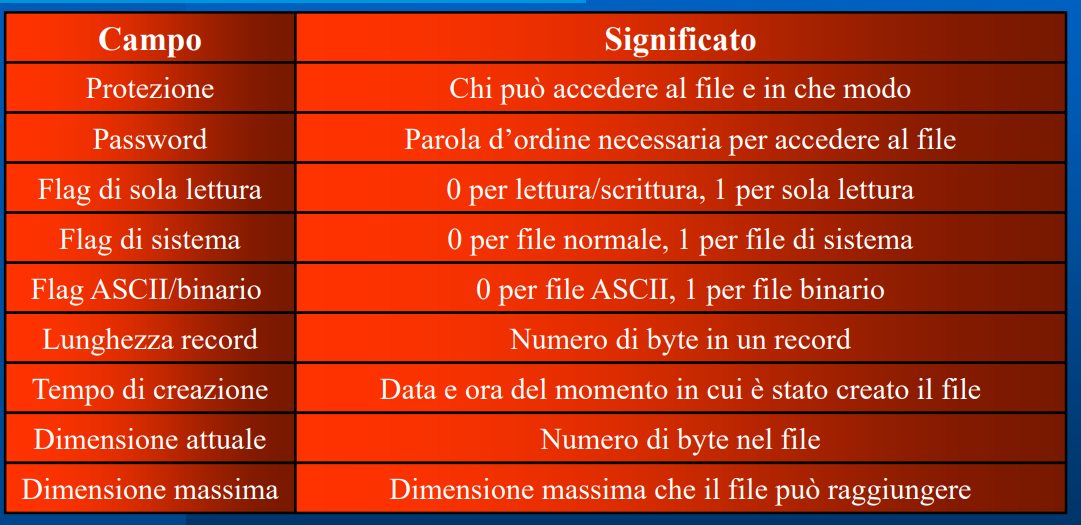
\includegraphics[width=1.00\textwidth]{Attributi_file}
	\end{figure}
	\section{Operazioni sui file}
	Il sistema operativo pone a disposizione dell'utente \textit{comandi di alto livello} e \textit{chiamate di sistema} per la gestione dei file. \\
	Alcune chiamate più comuni sono:
	\begin{itemize}
		\item \textbf{create}: creazione del file;
		\item \textbf{delete}: cancellazione del file;
		\item \textbf{open}: apertura del file con varia modalità;
		\item \textbf{close}: chiusura del file;
		\item \textbf{read}: lettura di blocchi di dati;
		\item \textbf{write}: scrittura di blocchi di dati;
		\item \textbf{append}: aggiunta, in coda al file, di nuovi dati;
		\item \textbf{seek}: posizionamento del puntatore all'interno del file.
	\end{itemize}
	\section{File mappati in memoria}
	Alcuni sistemi operativi, come Unix, consentono di \textbf{mappare} un file in memoria, ossia di caricarlo tutto o in parte, assegnandogli degli indirizzi virtuali. \\
	Questo permette ai processi di accedere in maniera trasparente ai file che possono essere contenuti in memoria centrale per intero o per blocchi. \\
	Questa tecnica velocizza le operazioni compiute sul file, soprattutto quando si riferiscono a parti limitate e non all'intero file. Quando il processo che sta usando il file termina, quest'ultimo viene riscritto sul disco. \\
	La virtualizzazione dell'accesso comporta alcuni problemi che vanno gestiti:
	\begin{itemize}
		\item in caso di apertura contemporanea del file da parte di più processi alcune informazioni possono risultare inconsistenti;
		\item in caso di caduta del sistema alcune informazioni possono essere perse;
		\item sono necessarie tecniche per la rimozione delle pagine o dei blocchi dei file.
	\end{itemize}
	\section{Directory}
	Per tenere traccia dei file, il file system fornisce un indice chiamato \textbf{directory}. \\
	I vecchi sistemi prevedevano un'unica directory in cui confluivano tutti i file ma questo concetto è stato superato dai \textbf{sistemi gerarchici di directory}. \\
	Tipicamente un elemento di directory contiene:
	\begin{itemize}
		\item il nome di un file ed eventualmente anche gli \textbf{attributi} del file;
		\item in alternativa, il nome di un file ed un \textbf{puntatore} ad un'altra struttura in cui si trovano gli attributi e gli indirizzi del disco.
	\end{itemize}
	Ogni directory può contenere:
	\begin{itemize}
		\item \textbf{file regolari};
		\item altre \textbf{directory}
	\end{itemize}
	In questo modo, a partire da un directory \textbf{radice} o \textbf{root directory} è possibile generare un albero di directory e \textbf{subdirectory}. Il tipo di organizzazione dell'albero delle directory dipende dalla scelta dell'amministratore di sistema. Un tipico esempio prevede:
	\begin{itemize}
		\item la root directory include alcune directory di sistema come \textit{etc, bin, lib, tmp,} ecc;
		\item la root directory include una o più directory come \textit{usr} per gli utenti;
		\item la directory \textit{usr} contiene una subdirectory per ogni utente che organizza il proprio sottoalbero nel modo che ritiene più efficiente e comodo per il tipo di attività che svolge.
	\end{itemize}
	Quando il file system è organizzato come un albero di directory, è necessario un qualche modo per specificare i nomi dei file. Questo può essere fatto in due diversi modi:
	\begin{itemize}
		\item \textbf{path name assoluto}: consiste nel cammino dalla directory radice al file. I componenti del cammini sono separati dal simbolo "/" in Unix e "\" in DOS.
		\item \textbf{path name relativo}: si usa congiuntamente al concetto di directory di lavoro. Un utente può definire una directory come \textit{directory di lavoro corrente}. In questo caso tutti i path name che non iniziano con la directory radice sono considerati relativi alla directory di lavoro. 
	\end{itemize}
	Alcune tipiche chiamate di sistema per la gestione delle directory sono:
	\begin{itemize}
		\item \textbf{create}: crea una directory vuota;
		\item \textbf{delete}: cancella una directory;
		\item \textbf{opendir}: apre una directory per leggere il contenuto;
		\item \textbf{closedir}: chiude una directory;
		\item \textbf{readdir}: restituisce il prossimo elemento di una directory vuota;
		\item \textbf{rename}: rinomina una directory;
		\item \textbf{link}: crea un link tra un file esistente ed una pathname;
		\item \textbf{unlink}: rimuove un elemento dalla directory.
	\end{itemize}
	\section{Implementazione del file system}
	Un fattore chiave nell'implementazione della memorizzazione dei file è tener traccia di quali blocchi del disco associare a ciascun file. \\
	Le modalità di allocazione dei blocchi e del relativo reperimento sono:
	\begin{itemize}
		\item \textbf{Allocazione contigua};
		\item \textbf{Allocazione a lista concatenata};
		\item \textbf{Allocazione a lista concatenata con indice};
		\item \textbf{Allocazione mediante uso di tabelle i-node}.
	\end{itemize}
	\subsection{Allocazione contigua}
	Questo è lo schema di allocazione più semplice, in quanto memorizza il file in blocchi di disco consecutivi
	\paragraph{Pregi} Questo modalità di allocazione è molto semplice da implementare poichè tiene traccia del solo indirizzo del file memorizzando, quindi, un solo numero ed è molto efficiente perchè permette di leggere l'intero file con una sola operazione
	\paragraph{Difetti} Non è realizzabile senza che si conosca la dimensione massima del file e il disco risulta notevolmente frammentato e molto spazio viene sprecato.
	\subsection{Allocazione a lista concatenata}
	Ogni blocco associato al file contiene:
	\begin{itemize}
		\item dati veri e propri;
		\item il numero del blocco successivo assegnato al file.
	\end{itemize}
	\paragraph{Pregi} Non implica spreco di spazio perchè i blocchi vengono allocati dinamicamente e nell'elemento delle directory viene memorizzato solo l'indirizzo del primo blocco.
	\paragraph{Difetti} La lettura sequenziale del file è semplice, ma l'accesso diretto ai blocchi è estremamente lento e la quantità di dati nel blocco non corrisponde più ad una potenza di due.
	\subsection{Allocazione a lista concatenata con indice}
	Assegna ai file:
	\begin{itemize}
		\item blocchi di disco non necessariamente contigui;
		\item mantiene l'elenco dei blocchi assegnati mediante una tabella in memoria.
	\end{itemize}
	Questo tipo di allocazione è utilizzata nel sistema operativo MS-DOS.
	\paragraph{Pregi} L'intero blocco è disponibile per i dati e l'accesso diretto ad un blocco è molto più rapido. Inoltre, l'elemento della directory contiene solo il numero del primo blocco.
	\paragraph{Difetti} Lo svantaggio principale consiste nel fatto che ad un gran numero di blocchi di disco corrisponde una tabella grande che occupa molto spazio in memoria centrale.
	\subsection{Allocazione mediante uso di tabelle i-node} Questo tipo di allocazione è utilizzata nel sistema operativo Unix. \\
	Gli i-node sono piccole tabella che contengono:
	\begin{itemize}
		\item  gli attributi del file;
		\item gli indirizzi dei primi dieci blocchi assegnati al file;
		\item tre campi che consentono l'indirizzamento dei blocchi successivi mediante:
		\begin{itemize}
			\item blocco a singola indirezione;
			\item blocco a doppia ed a tripla indirezione.
		\end{itemize}
	\end{itemize}
	Gli i-node sono in posizione definita all'interno del file system.
	\paragraph{Pregi} L'elemento di directory contiene solo il nome del file ed il numero di i-node e consente di mantenere in memoria gli i-node dei file aperti sprecando poco spazio. Inoltre, consente di indirizzare un numero enorme di blocchi di disco e per i file di piccole dimensioni consente di reperire rapidamente l'indirizzo dei primi blocchi di disco.
	\section{Struttura delle directory} 
	Il file system, mediante il \textit{pathname} fornito dall'utente:
	\begin{itemize}
		\item localizza l'elemento della directory;
		\item estrae le informazioni necessarie per trovare i blocchi di disco assegnati al file.
	\end{itemize}
	\section{Gestione dello spazio su disco}
	I file sono generalmente memorizzati su disco, pertanto la \textit{gestione dello spazio su disco} è uno dei problemi fondamentali nell'implementazione del file system. \\
	I file, generalmente, vengono memorizzati in blocchi di disco non necessariamente contigui. Questo perchè memorizzando un file con una sequenza contigua di byte si presenta l'ovvio problema che se il file aumenta di dimensione molto probabilmente dovrà essere spostato nel disco e lo spostamento di un file su un disco è un'operazione complessa e lenta.
	\subsection{Dimensione dei blocchi} 
	Il primo problema da risolvere è la scelta della dimensione dei blocchi. La scelta di un blocco molto grande rende più veloce il tempo di lettura ma provoca maggiore di spazio, invece, se la dimensione del blocco è molto piccola causa numerosi accessi ai blocchi per leggere i dati ma consente una gestione più efficiente dello spazio. \\
	L'efficienza nel tempo e nello spazio sono intrinsecamente in conflitto nella scelta delle unità di allocazione perchè ad una buona utilizzazione dello spazio corrisponde una bassa percentuale di dati e viceversa. \\
	Un compromesso si raggiunge scegliendo la dimensione del blocco di allocazione di 512 byte, 1024 byte e 2048 byte. \\
	Considerando che il \textit{settore} è la minima unità fisica leggibile dal disco avremo che la dimensione del settore su disco è generalmente di 512 byte e la lettura di un blocco di allocazione di un 1Kb causerà sempre la lettura consecutiva di due settori di disco.
	\subsection{Gestione dei blocchi liberi} 
	Il problema successivo alla scelta di dimensione del blocco è quello della gestione dei blocchi liberi. \\
	I metodi comunemente usati sono due:
	\begin{itemize}
		\item \textbf{lista concatenata} di blocchi che contengono gli indirizzi dei blocchi liberi nel disco;
		\item \textbf{mappa di bit}: un disco di \textit{n} blocchi richiede una mappa di \textit{n} bit. I blocchi si rappresentano con 1 sulla mappa e 0 quelli allocati o viceversa. 
	\end{itemize}
	Il metodo della lista concatenata è più efficiente se il disco è quasi pieno, poichè il numero di blocchi è molto limitato. Inoltre, in queste condizioni, la mappa di bit potrebbe risultare spesso piena e richiedere continui accessi ad altre parti di mappa per assegnare blocchi liberi. Se c'è abbastanza memoria principale per contenere la mappa di bit, è generalmente preferibile questo rispetto alla lista concatenata.
	\section{Affidabilità del file system}
	Il file system può contenere dati che non possono essere persi poichè di difficile o costoso recupero. L'affidabilità del file system va perseguita spesso anche a scapito dell'efficienza o di economie. 
	\subsection{Gestione dei blocchi fuori uso}
	I dispositivi di memorizzazione presentano spesso blocchi inutilizzabili a causa di urti violenti, usura o difetti di fabbricazione. I blocchi inutilizzati non devono essere assegnati a nessun file e devono essere gestiti appropriatamente. \\
	La soluzione per la gestione dei blocchi danneggiati possono essere di due tipi:
	\begin{itemize}
		\item \textbf{soluzioni hardware}: una parte di disco è riservata per tenere traccia dei blocchi rovinati e contiene dei blocchi di riserva. In fase di inizializzazione il controllore del disco legge questi blocchi e li sostituisce con blocchi di riserva, memorizzando l'avvenuta sostituzione. Questa soluzione è trasparente al file system.
		\item \textbf{soluzioni software}: l'utente o il file system tiene traccia dei blocchi rovinati assegnandoli tutti ad un file speciale da non utilizzare e nelle operazioni di backup è necessario porre attenzione per evitare le lettura di questo file. \\
		Ad esempio, il file system MS-DOS marca questi blocchi con un codice speciale 888 nella \textit{File Allocation Table} e questi blocchi non verranno mai assegnati.
	\end{itemize}
	\subsection{Copie di backup}
	Il metodo per ridurre le perdite di dati in caso di crash del file system è effettuare le copie di backup. \\
	Nella pianificazione delle operazioni di backup vanno valutati principalmente: 
	\begin{itemize}
		\item la frequenza con cui effettuare le copie di backup;
		\item i file che presentano la maggior necessità di essere copiati;
		\item la tecnica migliore per effettuare il backup.
	\end{itemize}
	\paragraph{Frequenza} La scelta va pianificata in base alla quantità di lavoro svolta nel tempo ed al costo di ripristino. Generalmente la frequenza è di tipo:
	\begin{itemize}
		\item Giornaliera;
		\item Settimanale;
		\item Mensile;
		\item Annuale.
	\end{itemize}
	\paragraph{Scelta dei file} La scelta va pianificata in base al contenuto dei file ed al costo di ripristino. Ad esempio:
	\begin{itemize}
		\item i file \textit{critici} potrebbero essere raggruppati in directory dedicate delle quali si effettua copia con maggiore frequenza;
		\item la duplicazione di alcuni file \textit{critici} può essere opportuna se il quantitativo di memoria sprecato è giustificabile. 
	\end{itemize}
	\paragraph{Tecniche di backup} La scelta va pianificata in base al tempo disponibile ed al costo sopportabile per i supporti. Le tecniche di backup possono essere:
	\begin{itemize}
		\item backup su nastri dell'intero file system;
		\item backup incrementale: copia solo dei file nuovi o modificati dall'ultimo backup;
		\item duplicazione incrociata dei dati su due dispositivi: metà di ogni disco contiene i propri dati e l'altra metà contiene i dati dell'altro disco.
	\end{itemize}
	\subsection{Consistenza del file system}
	 Nel corso della vita del file system può succedere che la sua consistenza venga a mancare a causa di crash, programmi che non rispettano le regole di allocazione o per altri motivi. La maggior parte dei sistemi operativi prevede un programma di servizio per la verifica della consistenza del file system e la correzione degli errori. \\
	 Ad esempio i controlli di consistenza di Unix sono di due tipi: sui blocchi e sui file.
	 \paragraph{Controllo di consistenza sui blocchi} Nell'effettuare il controllo di consistenza sui blocchi Unix usa una tabella con due contatori per ogni blocco: il primo registra quante volte il blocco è presente in un file e il secondo quante volte è presente nella lista libera. \\
	 Il test consiste nella scansione degli i-node, per individuare i blocchi assegnati e la scansione della lista dei blocchi liberi. Al termine del check si possono verificare i seguenti casi:
	 \begin{itemize}
	 	\item \textbf{caso normale}: un blocco è presenta una sola volta nella lista xor in un file;
	 	\item \textbf{blocco mancante}: un blocco non è presente nella lista libera e non è assegnato a nessun file, viene assegnato alla lista libera;
	 	\item \textbf{blocco duplicato nella lista libera}: il doppio riferimento viene cancellato;
	 	\item \textbf{blocco assegnato a due file:} è il caso più grave perchè è sintomo di possibili dati alterati. Il contenuto del blocco è copiato in un altro blocco ed ognuno dei blocchi assegnato ad un file;
	 	\item \textbf{blocco presente nella lista libera ed assegnato ad un file}: viene eliminato dalla lista libera.
	 \end{itemize}
	 \paragraph{Controllo di consistenza sui file} Unix quando effettua il controllo di consistenza sui file tiene conto che file distribuiti su diverse directory possono puntare allo stesso file fisico, e quindi allo stesso i-node, in tal caso il contatore di i-node è $>$ 1. Nel test l'albero delle directory viene interamente percorso e un contatore temporaneo per ogni i-node indica quanti file fanno riferimento ad ogni i-node. \\
	 I risultati che si possono verificare sono:
	 \begin{itemize}
	 	\item \textbf{risultato normale}: contatore temporaneo è uguale al contatore di i-node;
	 	\item \textbf{contatore temporaneo $<$ contatore di link}: anche se tutti i file vengono rimossi, l'i-node rimane bloccato e al valore del link viene assegnato il valore del contatore.
	 	\item \textbf{contatore temporaneo $>$ contatore di link}: se alcuni file vengono rimossi, il valore del link si azzera. L'i-node viene reso libero e i blocchi ad esso assegnati vengono assegnati alla lista libera. Inoltre, potrebbero esserci file che puntano erroneamente all'i-node e i dati vengono persi e il contatore di link viene aggiornato al valore attuale.
	 \end{itemize}
	\section{Prestazioni del file system} 
	L'accesso al disco è un'operazione notevolmente più lenta della lettura in memoria. Molti file system prevedono tecniche per ridurre il numero di accessi al disco come:
	\begin{itemize}
		\item \textbf{caching};
		\item \textbf{riduzione dei movimenti del braccio del disco} (soluzione soft);
		\item \textbf{riduzione dei movimenti del braccio del disco} (soluzione hard).
	\end{itemize}
	\subsection{Caching} Una delle tecniche più usate più comunemente è il \textit{block cache} in cui un certo numero di blocchi in memoria vengono riservati per contenere blocchi di disco. La quantità dei blocchi riservati va scelta in funzione della memoria utilizzata e del miglioramento delle prestazioni richieste. \\
	I principi operativi che la regolano sono:
	\begin{itemize}
		\item ad ogni richiesta di un blocco viene scandita la tabella di blocchi in memoria per verificarne la presenza;
		\item se non è presente il blocco viene caricato dal disco, copiato nella cache e poi reso disponibile alle richieste;
		\item la lista può essere gestita con normali algoritmi di rimpiazzamento delle pagine come FIFO o LRU;
		\item i blocchi critici vengono immediatamente riscritti sul disco quando modificati;
		\item per gli altri blocchi si può decidere di riscriverli subito oppure con una determinata frequenza.
	\end{itemize}
	\subsection{Riduzione dei movimenti del braccio del disco, soluzione soft} La riduzione dei movimento del braccio del disco avviene nei seguenti passi:
	\begin{itemize}
		\item \textbf{raggruppamento di blocchi in uso}: andando a stimare i bocchi a cui si accede con maggiore probabilità in sequenza, al fine di ridurre i movimenti della testina. Si può osservare che con la gestione con mappa di bit è più facile scegliere un blocco libero vicino al precedente.
		\item \textbf{posizione dell'indice dei blocchi}. Tenendo conto che la lettura di un file richiede un duplice accesso, uno all'i-node ed uno al blocco in modo da ridurre la distanza fra gli i-node e i blocchi a cui questi fanno riferimento;
		\item \textbf{partizioni aperte}: si tende ad avvicinare gli i-node ai blocchi cui fanno riferimento andando a dividere il disco in gruppi di cilindri, ognuno con i propri i-node e la propria lista dei blocchi liberi e quando una partizione esaurisce i blocchi, un blocco può essere allocato in una partizione diversa;
		\item \textbf{interleave}: un processo richiede un tempo $t_b$ per richiedere e recuperare un blocco. In situazioni di richieste consecutive un blocco richiesto può essere già passato sotto la testina e bisogna attendere una rotazione intera. \\
		La tecnica di interleaving alloca i blocchi fisici del disco in ordine non sequenziale stretto, ma sequenziale con salti. \\
		Sia $t_r$ il tempo di rotazione del disco avremo che:
		\[fattore\ di\ interleaving\ =\ \dfrac{t_r}{t_b} + 1\] 
	\end{itemize}
	\subsection{Riduzione dei movimenti del braccio del disco, soluzione hard} La riduzione dei movimenti del braccio del disco avviene mediante la \textit{schedulazione del braccio del disco}. Il tempo necessario per leggere un blocco di disco dipende da:
	\begin{itemize}
		\item \textbf{seek time}: spostamento della testina sul cilindro;
		\item \textbf{latency time}: tempo di rotazione per raggiungere il settore richiesto;
		\item \textbf{transfer time}.
	\end{itemize}
	Il ritardo predominante è dato dal seek time, per cui vari algoritmi sono stati ideati per ottimizzare il movimento del braccio delle testine. Alcuni esempi sono:
	\begin{itemize}
		\item \textbf{FCFS}: serve le richieste nell'ordine in cui giungono e non richiede nessun specifico supporto hardware o software. Questo è l'algoritmo più corretto nei riguardi delle richieste ma non ottimale perchè costringe il braccio del disco ad un superlavoro.
		\item \textbf{SSF (Shortest Seek First)}: mantenendo in tabella tutte le richieste pendenti, l'SSF si sposta sempre sulla richiesta più vicina a quella appena servita. Questo algoritmo riduce gli spostamenti sul disco ma presenta un problema di localizzazione delle richieste;
		\item \textbf{algoritmo dell'ascensore}: mantiene in tabella le richieste pendenti e presenta un bit up/down che indica la direzione attuale del braccio del disco e serve le richieste più vicine proseguendo sempre nella stessa direzione e cambia direzione quando non ci sono più richieste in quella direzione o quando raggiunge l'estremità. Questo algoritmo concilia meglio equità di servizio con efficienza.
	\end{itemize}
	\section{Modelli di protezione} Gli utenti operano sugli archivi per mezzo dei processi di loro proprietà: le operazioni eseguibili dal generico processo sono limitate dai diritti di accesso attribuiti al suo proprietario. Le politiche che regolano l'attribuzione dei diritti d'accesso spetta al sistema operativo o all'utente medesimo. \\
	Spetta, invece, al file system realizzare i meccanismi di protezione che impediscono agli utenti di superare i limiti dei propri diritti di accesso. \\
	\section{Dominio di protezione} Un modello generale di questi meccanismi è basato sul concetto di \textit{dominio di protezione}. Un dominio di protezione è un insieme di coppie del tipo (Oggetto, DirittiDiAccesso). \\
	Ad esempio:
	\begin{itemize}
		\item ($F_i$, \{r,w\}) esprime il possesso di lettura e di scrittura sull'archivio $F_i$.
	\end{itemize}
	Il modello basato sui domini consente di formalizzare il concetto della migrazione dei processi in un dominio di protezione diverso da quello di appartenenza. Per formalizzare la facoltà di migrare da un dominio all'altro è sufficiente considerare anche i domini come oggetti ai quali è associata l'operazione di ingresso \{in\}. Una volta entrato in un nuovo dominio, l'utente o il processo proveniente da un altro dominio non ha la possibilità di migrare ulteriormente.
	\subsection{Strutture dati per la protezione} La matrice di protezione è tipicamente molto grande e sparsa. Una struttura più sufficiente è ottenuta rappresentando le stesse informazioni attraverso: 
	\begin{itemize}
		\item \textbf{liste di controllo degli accessi};
		\item \textbf{liste associate ai domini}.
	\end{itemize}
	\paragraph{Liste di controllo degli accessi} Ogni lista è associata ad un oggetto ed i suoi elementi sono coppie del tipo (dominio, insieme dei diritti di accesso). Ciascuna lista elenca tutti i diritti di accesso sull'oggetto che competono ad un certo dominio. Queste liste solitamente sono riferite agli utenti che sono identificati con una coppia del tipo (gruppo, nome) dove i nomi sono locali ai gruppi. Ogni lista è un attributi degli archivi.
	\paragraph{Liste associate ai domini} In questo caso ogni lista è associata ad un dominio e i suoi elementi sono coppie del tipo (oggetto, insieme dei diritti di accesso) dove ogni elemento della lista esprime la facoltà dell'utente di accedere ad un dato oggetto con i diritti compresi in un certo insieme. Ogni lista è un attributo degli utenti e dei loro processi.
	
	\section{Protezione nel sistema operativo UNIX}
	I meccanismi di protezione adottati in UNIX si basano sulle liste di controllo degli accessi. Dato che ogni processo è attribuito ad un utente proprietario, l'identificazione degli utenti si propaga ai loro processi. \\
	Ogni descrittore di archivio contiene una struttura dati simile, dal punto di vista del contenuto informativo ad una lista di controllo degli accessi. Essa consiste di tre codici:
	\begin{itemize}
		\item DirittiProprietario;
		\item DirittiGruppo;
		\item DirittiAltriUtenti.
	\end{itemize} 
	che esprimono i diritti di lettura, scrittura ed esecuzione agli utenti proprietari, agli utenti del gruppo e agli utenti degli altri gruppi. \\
	Questa convenzione non permette di discriminare tra utenti dello stesso gruppo del proprietario ne tra quelli appartenenti a gruppi diversi da quello del proprietario. \\
	\section{Identificazione degli utenti}
	I meccanismi di protezione degli archivi sono basati sul presupposto della sicura identificazione degli utenti. \\
	Nei sistemi interattivi multi-utente, il progenitore di tutti i processi di un generico utente è quello che viene generato quando esso si connette al sistema attraverso un terminale. \\
	Per ogni processo diverso dal progenitore, la responsabilità di definire il proprietario spetta al sistema operativo, che assegna il figlio allo stesso utente che risulta proprietario del processo padre. L'identificazione del proprietario del figlio è sicura se lo è quella del padre. \\
	La sicurezza degli archivi è fondata sulla corretta definizione del proprietario del processo progenitore, che dipende dalla sicura identificazione dell'utente che si connette attraverso il terminale. \\
	La tecnica comunemente usata è quella della password, che l'utente deve trasmettere attraverso il terminale, insieme al nome con il quale è registrato nel sistema, ogni volta che si connette.
\end{document}